% !TeX program = lualatex
\documentclass[a4paper,12pt]{article}
\usepackage{graphicx}
\usepackage{./style/head}     % Add local fullpage and head macros
\parindent=0pt          %  Switch off indent of paragraphs 
\parskip=5pt            %  Put 5pt between each paragraph  
\usepackage{fontspec}
\usepackage[english]{babel}
\usepackage{setspace}
\setstretch{1.5}
\usepackage{libertinus}
\setmainfont{Libertinus Sans}
\renewcommand*\familydefault{\sfdefault} %% Only if the base font of the document is to be sans serif
%\usepackage{mathpazo}
%\usepackage{domitian}
%\usepackage[T1]{fontenc}
%\let\oldstylenums\oldstyle
\usepackage{enumerate}
\usepackage[
pdfauthor={Patrick Wang},
pdftitle={Patrick Wang MChemPhys Thesis},		
pdfsubject={Improving the Accuracy of Flux Calculations in Ray Tracing Simulations For Soft X-Ray Beamlines},
pdfproducer={LaTeX with hyperref},
pdfcreator={LuaLaTeX}]{hyperref}
\usepackage{booktabs}
\usepackage{physics}
\usepackage{amsmath}
\usepackage[capitalise]{cleveref}
\usepackage{tikz}
\usepackage{mathdots}
%\usepackage{yhmath}
\usepackage{cancel}
%\usepackage{color}
\usepackage[table,xcdraw]{xcolor}
\usepackage{siunitx}
\usepackage{pgf}
\usepackage{array}
\usepackage{multirow}
%\usepackage{amssymb}


\usepackage{gensymb}
\usepackage{tabularx}
\usepackage{extarrows}
\usepackage{booktabs}
\usepackage{textgreek}
\usepackage{multicol}
\usepackage{float}
\usetikzlibrary{fadings}
\usetikzlibrary{patterns}
\usetikzlibrary{shadows.blur}
\usetikzlibrary{shapes}
\hypersetup{
	colorlinks,
	linkcolor = {blue!50!black},
	citecolor={green!50!black}
}
\usepackage{physics}
\usepackage{amsmath}
\usepackage{tikz}
\usepackage{mathdots}
%\usepackage{yhmath}
\usepackage{cancel}
\usepackage{color}
\usepackage{siunitx}
\usepackage{array}
\usepackage{multirow}
%\usepackage{amssymb}
\usepackage{gensymb}
\usepackage{tabularx}
\usepackage{extarrows}
\usepackage{booktabs}
\usetikzlibrary{fadings}
\usetikzlibrary{patterns}
\usetikzlibrary{shadows.blur}
\usetikzlibrary{shapes}
\newcommand{\cff}{\mathit{c_{ff}}}
\usepackage[labelfont={bf, it}]{caption}
\usepackage[top=2.5cm, bottom=3cm, left=2cm, right=2cm]{geometry}
\usepackage{acro}
\renewcommand{\vec}{\vb}
\newcommand{\shadow}{\textit{SHADOW}}
\DeclareAcronym{mx}{short=MX, long=Macromolecular crystallography,short-format = \textsc}
\DeclareAcronym{ep}{short=EP, long=Experimental phasing,short-format = \textsc}
\DeclareAcronym{xrd}{short=XRD, long=X-ray diffraction, short-format = \textsc}
\DeclareAcronym{sad}{short=SAD, long=single-wavelength anomalous scattering,short-format = \textsc}
\DeclareAcronym{mad}{short=MAD, long=multi-wavelength anomalous scattering,short-format = \textsc}
\DeclareAcronym{ac}{short=AC, long=absorption correction,short-format = \textsc}
\DeclareAcronym{sh}{short=SH, long=Spherical harmonics,short-format = \textsc}
\DeclareAcronym{aac}{short=AAC, long=analytical absorption corrections,short-format = \textsc}
\DeclareAcronym{acsh}{short=ACSH, long=analytical correction with spherical harmonics,short-format = \textsc}
\DeclareAcronym{t1}{short=Tlys 1, long=Thermolysin 1,short-format = \textsc}
\DeclareAcronym{t2}{short=Tlys 2, long=Thermolysin 2,short-format = \textsc}
%\DeclareAcronym{xas}{short=XAS, long=X-ray absorption spectroscopy,short-format = \textsc}
%\DeclareAcronym{xes}{short=XES, long=X-ray emission spectroscopy,short-format = \textsc}
%\DeclareAcronym{xanes}{short=XANES, long=X-ray absorption near-edge structure,short-format = \textsc}
%\DeclareAcronym{exafs}{short=EXAFS, long=extended X-ray absorption fine structure,short-format = \textsc}
%\DeclareAcronym{pgm}{short=PGM, long={plane grating monochromator},short-format = \textsc}
\DeclareAcronym{id}{short=id, long=insertion device, short-format={\textsc}}
\acsetup{make-links = true}
\usepackage{multicol}
\newcommand\numberthis{\addtocounter{equation}{1}\tag{\theequation}}
\usepackage{mathtools}
\usepackage[style=phys,backend=bibtex]{biblatex}
\usepackage{fixltx2e}
\usepackage{booktabs}
\usepackage{multirow}


%\newcommand{\detailtexcount}[1]{%
  %\immediate\write18{texcount -merge -sum -q #1.tex output.bbl > #1.wcdetail }%
  %\verbatiminput{#1.wcdetail}%}
%\detailtexcount{main}

\addbibresource{export.bib}%cite.bib
\graphicspath{ {plots/} }
\newcommand{\hkl}{hk\ell}

\begin{document}
\pagenumbering{roman} 




\thispagestyle{empty}
\par\noindent                                           % Centre Title, and name

\begin{singlespace}
	\vspace{1cm}
	\begin{center}
		\Huge\bf\sc Absorption Correction using X-ray Tomography in Long-wavelength Macromolecular Crystallography \\
		\vspace{2mm}
		\large\bf Chemical Physics 5P Thesis
	\end{center}
	\vspace{1cm}
	\begin{center}
		
\includegraphics[width=70mm]{UoECentred.eps}
	\end{center}
	\vspace{1.8cm}
	\begin{center}
		\bf\Large Tihana Stefanic\\                 % Replace with your name
		April 2024                         % Submission Date
	\end{center}
	
	%\vspace*{1.5cm}
	\begin{center}
		\small\itshape
		Submitted in partial fulfilment of the requirements \\  for the degree of Master of Chemical Physics (Hons) \\
		to the \\
		School of Chemistry \\
		College of Science and Engineering \\
		University of Edinburgh
	\end{center}
	
	
	\vspace*{5mm}   

	
	\vspace*{3cm}
	
	
	\vfill
	{\bf Total combined wordcount:} \\
	{\bf Supervisors:} Dr Ramona Duman, Dr Armin Wagner, and Professor Caroline Kirk              % Change to suit
\end{singlespace}

\newpage
%                                               Through page and setup 
%                                               fancy headings
%\setcounter{page}{1}                            % Set page number to 1
\footruleheight{1pt}
\headruleheight{1pt}
\lfoot{\small School of Chemistry}
\lhead{Chemical Physics 5P Thesis}
\rhead{\thepage}
\cfoot{}
\rfoot{1\textsuperscript{st} April, 2024 }

%

\newpage
\setcounter{page}{1}
\section*{Declaration}
The contents of this report have been approved by the supervisor running this project and I declare the work as a non-confidential project.\\\\
I declare that this thesis was composed by myself, that the work contained herein is my own except where explicitly stated otherwise in the text, and that this work has not been submitted for any other degree or qualification. \\
\bigskip


\begin{flushright}
	\begin{tabular}{m{5cm}}
		\\ \hline
		\centering Tihana Stefanic \\
		
	\end{tabular}\\
	
	\raggedleft\textit{Oxford, April 2024}
\end{flushright}
\newpage

\section*{Acknowledgements}

I would like to acknowledge and give my sincerest gratitude to my supervisors, Ramona and Caroline, for their unwavering support throughout this project.

I thank Ramona for her time and patience in teaching me everything I know about this project, and for providing the knowledge and insight crucial to its success.

I thank Caroline for her time in reading over the draft and providing helpful feedback throughout the year.

I thank Kamel El Omari for sharing his novel work and insight into \textit{Phenix} refinement, thanks to which the ion identification experiment in this project was made possible.

I would like to thank Christian Orr for his consistent support in answering questions about beamline I23 and otherwise, debugging my codes, laser-shaping, and for training me in too many things to list here. %crystal-fishing, sample loading, laser-shaping, and

I am very grateful to my friends and colleagues, Patrick and Ismay, for their companionship and academic support throughout these experiments.
\newpage

\newpage

\printacronyms[template=description]
\newpage
\begin{abstract}
	Beamline I23 is a synchrotron instrument specifically designed for the study of long wavelength macromolecular crystallography experiments. The instrument operates in the wavelength range 1.5-5.9 Å (2.1 - 11.5 \unit{keV}), enabling the detection of X-ray absorption edges of biologically relevant light elements often found in proteins. Access to these absorption edges is of particular importance to macromolecular crystallography as they provide crucial information for determining the structures and ions bound to macromolecules in the form of anomalous scattering.
    While I23 is a specialised beamline for operating in-vacuum to provide high signal-to-noise ratios at the longest wavelengths, low-energy diffraction is still hindered by drastic absorption effects that must be accounted for from the samples themselves. In response, I23 operates an X-ray tomography camera to reconstruct a 3D model of samples, allowing for the calculation of X-ray path lengths to determine analytical absorption correction factors.
    This project explores the effects of tomography-based reconstructions for measuring absorption coefficients and its applications in further experiments at I23. This approach was combined with laser-shaping to assess the effects of combining two independent techniques of absorption corrections.
\end{abstract}
\newpage
\tableofcontents                                % Makes Table of Contents
\newpage


\listoffigures
\listoftables
\newpage

\pagenumbering{arabic}
%TC:subst \shadow SHADOW
\section{Introduction}


\ac{mx} is a powerful tool for determining the three-dimensional structures of biological molecules at atomic resolutions \cite{Gorrec2021}. It has contributed significantly to our understanding of structure-function relationships in biology, protein folding, enzyme mechanisms, and structure-based drug-design \cite{Foerster2019}. Today, most of \ac{mx} is carried out at synchrotron beamlines due to the high brilliance and wavelength-tunability of synchrotron radiation, which are important features to crystallography experiments.

Beamline I23 at Diamond Light Source, the UK's national synchrotron, is a specialised synchrotron instrument operating at a wavelength range beyond that of standard \ac{mx} beamlines. While absorption is a minor effect in standard \ac{mx}, it becomes the largest source of error at increasingly long wavelengths. For this reason, I23 houses a tomography camera to analytically correct absorption coefficients from the sample in a diffraction experiment.
%Experiments are becoming more difficult and people are observing diminishing returns on their experimental data; this is met with efforts in developing more complex equipment. The demands for optimising the usage of these novel apparatuses directly drive the development of complex physical models. Coupled with the advent of powerful computers, the relevance of X-ray ray tracing simulations in designing better experimental equipment is evergrowing. The importance of which will only increase in light of new developments in free electron lasers and 4\textsuperscript{th} generation synchrotrons.


%In this section, the basic principles of synchrotron radiation are introduced, along with its applicability in the chemical sciences. An introduction to the pgm and the ray-tracing technique is discussed to highlight challenges of simulating pgm. This sets the stage for understanding specifically the challenge of higher harmonic contamination in soft X-ray beamlines and the detrimental effect it can have on the quality of the data. All of which serve to provide the motivation for developing more robust ray-tracing methodologies that would hopefully resolve potential issues in future beamlines from the outset. 
In this section, the basic principles of \ac{mx} phasing by anomalous diffraction are introduced, along with its applicability in long-wavelength crystallography at beamline I23. This sets the stage for understanding the challenges associated with long-wavelength crystallography and the need for more sophisticated absorption correction techniques to exploit the full potential of long-wavelength crystallography. % its full potential
All of this serves to provide the motivation for developing more robust, analytical absorption correction methods that would hopefully improve data quality and structure determination in future \ac{mx} experiments limited by high absorption.

%The data reduction techniques used to determine structure factor amplitudes and their uncertainties in \ac{xrd} are affected by factors like geometry, sample illumination, and X-ray absorption. 

% I23 uses novel approach of X-ray tomography coupled with a ray-tracing software for calculating absorption correction analytically. This paper discusses the findings of using an analytical approach to absorption corrections compared to standard empirical methods, as well as the combination of the methods. We go on to investigate whether this approach improves data in the ion identification experiments performed at I23.
%Furthermore, we investigate a second, more robust approach to absorption correction using laser-shaping to remove a majority of the non-diffracting material from the sample; this method is tested both empirically and analytically to determine whether there is a qualitative improvement in the combination of X-ray tomography-based segmentation and laser-shaping.

\subsection{Experimental Phasing in Macromolecular Crystallography}

%\ac{xrd} experiments provide the diffraction patterns of a crystal from the constructive interference of X-rays scattered by its electron clouds. Fourier methods are then implemented to calculate Fourier difference maps and to extract electron density maps from the diffraction spots. The resulting three-dimensional electron density $\rho$ for a given reflection $\hkl$, at position $(x,y,z)$ in a unit cell of volume $V$  can be expressed as: \cite{Taylor2003}

%\begin{equation}
    %\rho(x,y,z)=\frac{1}{V} \sum |F_{\hkl}| \exp(i\alpha_{\hkl}) \exp(-2\pi i [hx+ky+\ell z]) \label{electron_density}
%\end{equation}

%Where the atomic structure factor, $F_{hkl}$, is a measure of how efficiently each atom scatterers X-rays relative to an electron, given by:

In \ac{xrd} experiments, the diffraction patterns of a crystal are provided by constructive interference of X-rays scattered by the electron clouds. These patterns elucidate vital structural information about the crystal in the form of electron density maps, which can be extracted using Fourier methods. Our ability to solve for electron density, given by \cref{electron_density}, is hampered by the \textit{phase problem}, wherein the phases $\alpha_{\hkl}$ for a given reflection $\hkl$ are not directly solvable in experiment. 

%\begin{equation}
    %\mathbf{F}_{\hkl}= |F_{\hkl}| \exp{i \alpha_{\hkl}} = \sum_j f_j \exp{[2\pi i (hx_j + ky_j + lz_j]}
    %\label{structure_factor}
%\end{equation}

%And where $\alpha_{hkl}$ is the associated phase, $f_j$ is the scattering factor of atom \textit{j}, and $x_j, y_j, z_j$ are its positional coordinates.

%In \ac{xrd}, the intensities of reflections are proportional to the square of the structure factor amplitudes ($I_{\hkl} \propto |F_{\hkl}|^2$). The amplitudes are therefore directly measurable from reflection intensities, while the phase $\alpha_{\hkl}$ is lost in experiment \cite{Taylor2003}.
%This results in the\textit{ phase problem} as there is no unique solution to \cref{electron_density} without knowing $\alpha_{hkl}$. %Phases therefore carry important structural information that is necessary for producing accurate electron density maps.

\begin{equation}
    \rho(x,y,z)=\frac{1}{V} \sum |F_{\hkl}| \exp(i\alpha_{\hkl}) \exp(-2\pi i [hx+ky+\ell z]) \label{electron_density}
\end{equation}
% prop to square root of refkection intensity
%a measure of how efficiently each atom scatterers X-rays relative to an electron
\cref{electron_density} illustrates how electron density is proportional to the amplitude of the atomic structure factor, $F_{hkl}$, a measure of the scattering power for reflection $\hkl$. Here, $x,y,z$ are the positional coordinates of reflection $\hkl$ in a unit cell of volume $V$, where $\hkl$ are the Miller indices describing the orientation of the crystal plane in reciprocal space. %by quantifying its reciprocal intercepts in the crystal axes.

\ac{ep} is concerned with solving the phase problem to extract structural information from diffraction experiments. One set of techniques which have become the preferred phasing methods in \ac{mx} rely on anomalous scattering, a phenomenon observed in the X-ray absorption of matter.

Anomalous scattering occurs when an incident X-ray has a wavelength close to an element’s absorption edge, leading to the photon being absorbed instead of scattered. A possible outcome of anomalous scattering is fluorescence, when higher energy electrons drop to lower energy shells. The more common outcome, most relevant to the present case, is the immediate re-emission of radiation, resulting in an imaginary phase shift. This causes the overall atomic scattering factor $f$ to experience a change in amplitude, described by a real dispersive term $f’$, and a change in phase, described by an imaginary absorptive term $f”$:

\begin{equation}
    f=f^0+f'(\lambda)+if''(\lambda) \label{total scattering}
\end{equation}

This behaviour is element-specific and exhibits a strong dependence on the wavelength of the incident radiation, making the phenomenon particularly useful for element identification as well as phasing.

\begin{figure}
    \centering
    \input{./images/Normal and anomalous scattering.txt}
    \caption{(A) Normal scattering: Friedel's law is obeyed; (B) Breakdown of Friedel's law in the presence of an anomalous scatterer; the amplitudes of reflections are given by $F_P$ for the native crystal and $F_{PH}$ for the derivative. The isomorphous difference, $F_H \approx F_{PH} - F_P$, is an estimate of the heavy-atom structure. Adapted from Taylor, G. \cite{Taylor2003}.}
    \label{Breakdown of Friedel's law}
\end{figure}
% add side-by-side picture of Friedel's law obeyed
% replace labels with f = f0 + f' + if"

\ac{ep} by anomalous diffraction takes advantage of the differences in amplitude between Friedel pairs to determine the phase angles. In \ac{mad}, phases are determined using the orthogonal information from anomalous dispersion recorded at multiple wavelengths, while \ac{sad} requires phase ambiguity resolution either in the form of a structural derivative labelled with an anomalous scatterer (\textit{i.e.} selenomethionine), or using the anomalous signal of  natively present atoms in what is known as native \ac{sad}.

Native \ac{sad} is considered an attractive phasing technique in  \textit{de novo} X-ray structure determination %in MX,
for exploiting weak signals from intrinsic anomalous scatterers \cite{Basu2019}, with its most popular applications being on native sulphur and phosphorous \cite{Karasawa2022}. However, native \ac{sad} has its challenges in \ac{mx}, largely owing to the fact that standard beamlines are optimised around the selenomethionine K-edge of 12.7 keV (0.979 Å) to allow for experiments on Se-incorporated proteins.
While the edges of metalloproteins therefore typically lie in the accessible wavelength range of most standard \ac{mx} beamlines (0.9-2.5 Å), several light atoms native to nucleic acids and proteins (including sulphur and phosphorous), have absorption edges beyond the reach of most current \ac{mx} beamlines (5.02 Å and 5.78 Å respectively) \cite{Olieric2016}. 

%thus
Native \ac{sad} is in turn typically performed at 'compromise' energies of around 6 keV, which is far from the absorption edges of the aforementioned light atoms. The resulting anomalous signal is small and systematic errors from radiation damage need to be minimised to accurately measure reflection intensities \cite{DjinovicCarugo2005}.%(Djinovic-Carugo, 2005). %This renders many biologically useful native SAD experiments inaccessible to most MX beamlines. 

Data collection at energies lower than 6 keV is attractive for the native \ac{sad} phasing of macromolecules for this reason. This is epitomised by beamline I23 at Diamond Light Source, arguably the most specialised \ac{mx} beamline in the world \cite{Foerster2019}. %In addition to phasing, another use of anomalous diffraction is for ion identification, which is another primary focus of beamline I23.

\subsection{Beamline I23: Long-wavelength Macromolecular Crystallography}

Diamond Light Source (DLS) is a third generation, medium energy synchrotron based in the United Kingdom. It houses 32 beamlines, each using synchrotron light to investigate different subjects including protein structure, materials, and engineering innovations.
I23 is a unique long-wavelength \ac{mx} beamline capable of operating at wavelengths between 1 and 5.9 Å \cite{Wagner2016}.

The wavelength range at I23 covers the absorption edges of
%several anomalous scatterers of biological importance, such as sulphur, potassium, chlorine, and phosphorous. 
light elements often present in macromolecules (P, S, Cl, K, Ca, Mg).
Native \ac{sad} experiments performed at I23 enable \ac{ep} without the need for additional labelling by exploiting the anomalous scattering from these atoms at sufficiently long wavelengths.
%the need for derivatives such as selenomethionine.
Collection wavelengths can be tuned to closely above and below the absorption edges, also enabling identification of the element type and location; an example of this application in experiment is known as $f"$-refinement, which is used for ion identification at I23. % anomalous scattering at I23.%where the experimentally determined $f"$ elucidates the atom type. %this is the primary application of anomalous scattering at I23. %Ion identification using anomlous scattering is therefore a large focus of I23.

\begin{figure}[h]
    \centering
    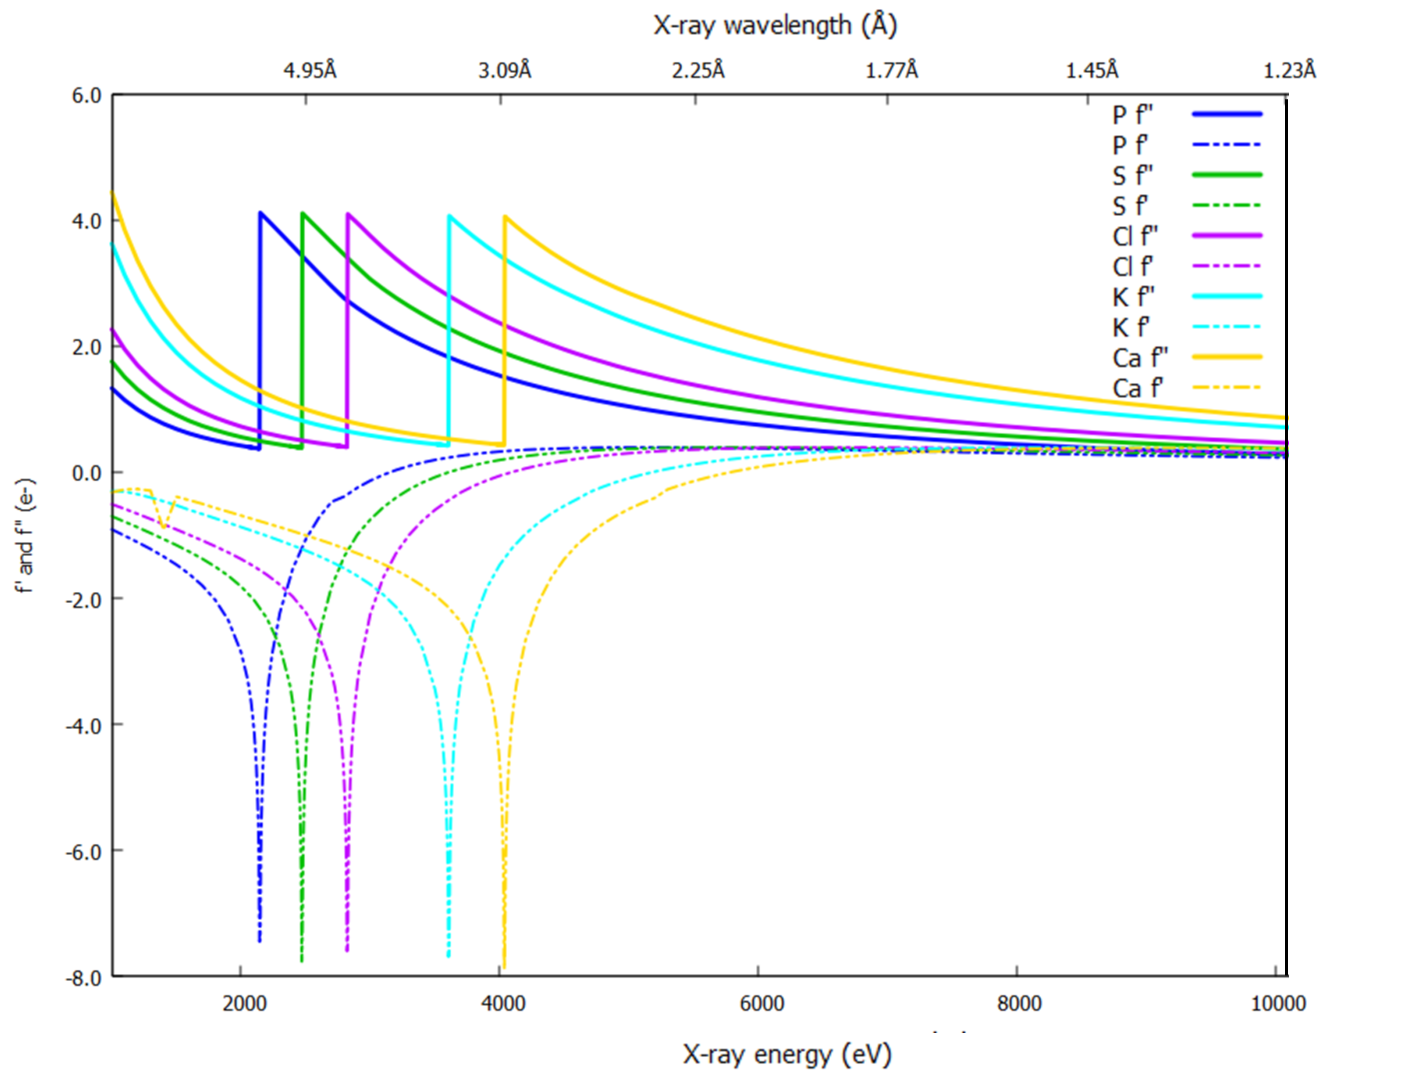
\includegraphics[width = 0.65\textwidth]{images/absorption lines high quality cropped.png}
    \caption{Characteristic X-ray absorption lines of biologically relevant elements (P, S, Cl, K, Ca) accessible at I23 beamline energy range. Adapted from the \href{http://skuld.bmsc.washington.edu/scatter/AS_periodic.html}{X-ray Absorption Edges} platform using the subroutine library by Brennan and Cowan \cite{Brennan1992}.}%anomalous scatterers common in macromolecules (P, S, Cl, K, Ca), showing the real dispersive term $f'$ and imaginary absorptive term $f''$. NB elements of a lower atomic number have emission lines at longer wavelengths. Produced by Brennan and Cowan. \cite{Brennan1992} }%NB the emission wavelength is critically affected by the molecular environment, and therefore unique to every atom in a structure.}
    \label{Anomaluos scattering edges}
\end{figure}

The need for the beamline's specialised operation stems from the complex challenges of operating at such low energies, which greatly obstruct the quality of diffraction experiments.
%Low-energy \ac{xrd} is hindered by 
One source of hindrance is Bragg’s law, $nλ = 2d \sin(\theta)$, which states that the diffraction angle increases with wavelength. The highest resolution X-rays can therefore go unrecorded if they pass beyond the reach of the detector. The solution to this on I23 is a semi-cylindrical detector, the Pilatus 12M shown in \cref{fig:gonio_and_detector} (right), which allows most of the data to be detected. Nevertheless, data resolution is still limited by the detector’s geometry at the longest wavelengths.

 Another challenge is that sample absorption is approximately proportional to the cube of the wavelength, $\mu \propto \lambda^3$ \cite{Arndt1984}, making it a crucial limiting factor at long-wavelengths. The effects not only contribute to radiation damage, but also attenuate the diffracted X-rays within the sample \cite{Wagner2016}.

To eliminate the adverse absorption of low-energy X-rays by gases, experiments are performed in-vacuum at temperatures below 100 K. This setup requires a dedicated endstation for the transfer of frozen samples from air to a vacuum environment. By operating in-vacuum at cryogenic temperatures, I23 eliminates air absorption and scattering while reducing radiation damage, increasing the signal-to-noise ratio even at the lowest energies.

\begin{figure}
    \centering
    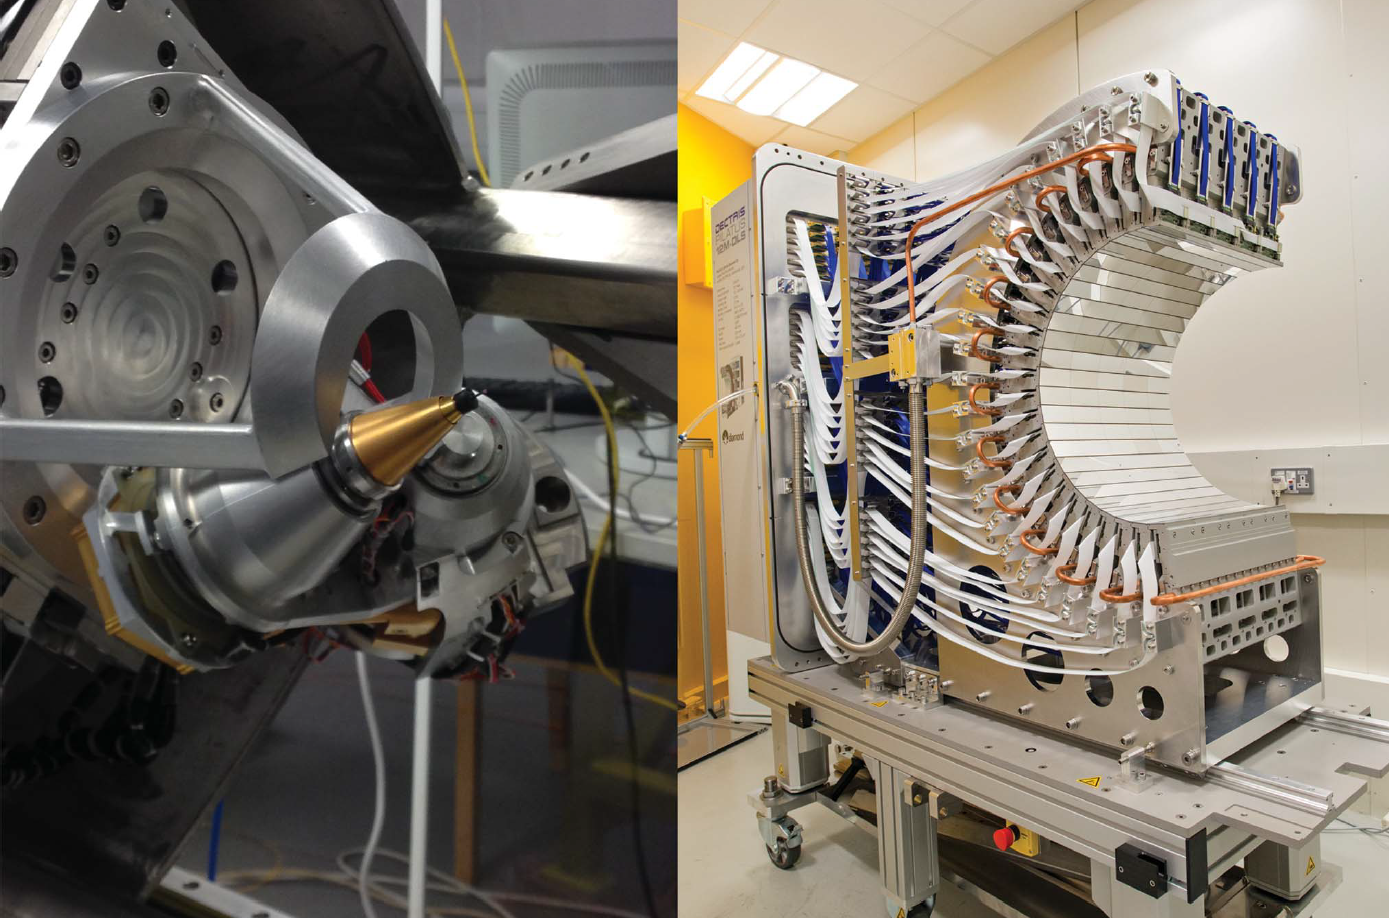
\includegraphics[width = 0.7\textwidth]{images/goniometer&detector.PNG}
    \caption{The kappa goniometer of the I23 endstation (left) and the Pilatus 12M before installation (right). Produced by Wagner \textit{et al.} \cite{Wagner2016}}
    \label{fig:gonio_and_detector}
\end{figure}

% pictures of endstation + vacuum chamber + detector + crystream

Nevertheless, absorption effects remain drastic at the longest wavelengths, and a correction is needed in response \cite{Kazantsev2021}.

\subsection{Absorption Correction Techniques at I23}

%The data reduction techniques used to determine structure factor amplitudes and their uncertainties in \ac{xrd} are affected by factors like geometry, sample illumination, and X-ray absorption. While the latter is a minor effect in standard MX, absorption becomes the largest source of error at increasingly long wavelengths.

%Away from absorption edges, the absorption of a sample is approximately proportional to the cube of the wavelength, $\mu \propto \lambda^3$ \cite{Arndt1984}. \ac{xrd} at long-wavelengths is therefore hindered by high absorption effects, such as X-ray scattering by air and low diffraction intensities. I23 mitigates some of these effects by operating in-vacuum, thereby increasing the overall signal-to-noise ratio.

%Another issue of low-energy MX stems from Bragg’s law, $nλ = 2d \sin(\theta)$, which states that the diffraction angle increases with wavelength. The highest resolution X-rays can therefore go unrecorded if they pass beyond the reach of the detector. The solution to this on I23 is a semi-cylindrical detector, Pilatus 12M, which allows most of the data to be detected. Nevertheless, data resolution is still limited by the detector’s geometry at the longest wavelengths.%, and several factors need to be considered to calculate structure factor amplitudes.

%Since high-quality structure determination relies on accurate structure factor amplitudes, 

Accounting for the absorption effects on Bragg’s intensities becomes critical at long wavelengths. For a lone crystal sample, the measured intensities corrected for absorption are given by $I_{corr} = I_{measured}/A_{\hkl}$, where the absorption correction factor, $A_{\hkl}$, for the reflection $\hkl$ is given by \cite{Albrecht1939}: %(Albrecht, 1939):

\begin{equation}
    A_{\hkl} = \frac{1}{V} \int_V \exp{-\mu(L_1+L_2)} dV
    \label{AbsFactor}
\end{equation}

Where $L_1$ and $L_2$ are the incident and diffracted X-ray paths for each crystal element $dV$ respectively, and $\mu$ is the X-ray absorption coefficient. \cite{Busing1957}

In a standard \ac{mx} experiment, X-rays transmit not only through the diffracting material but also the sample mount and surrounding solvent. This non-diffracting material is accounted for by expressing the absorption factor as:

\begin{equation}
    A_{\hkl} = \frac{1}{V} \sum_i \exp{-\mu_i (L_{1,i}+L_{2,i})} dV
    \label{AbsFactor_allmaterials}
\end{equation}

Where the sum is over $i$ materials exposed to the X-rays \cite{Santoro1968}. This analytical approach however requires precise information on the geometry of sample.

Absorption corrections are typically performed using empirical methods based on spherical harmonics \cite{Blessing1995}. \ac{sh} estimate the radii of spherical crystals to minimise differences between symmetry-related reflection intensities, with the first few models visualised in \cref{fig:SH}. %These models inherently assume a spherical shape of the diffracting material in question in data reduction.


\begin{figure}
    \centering
    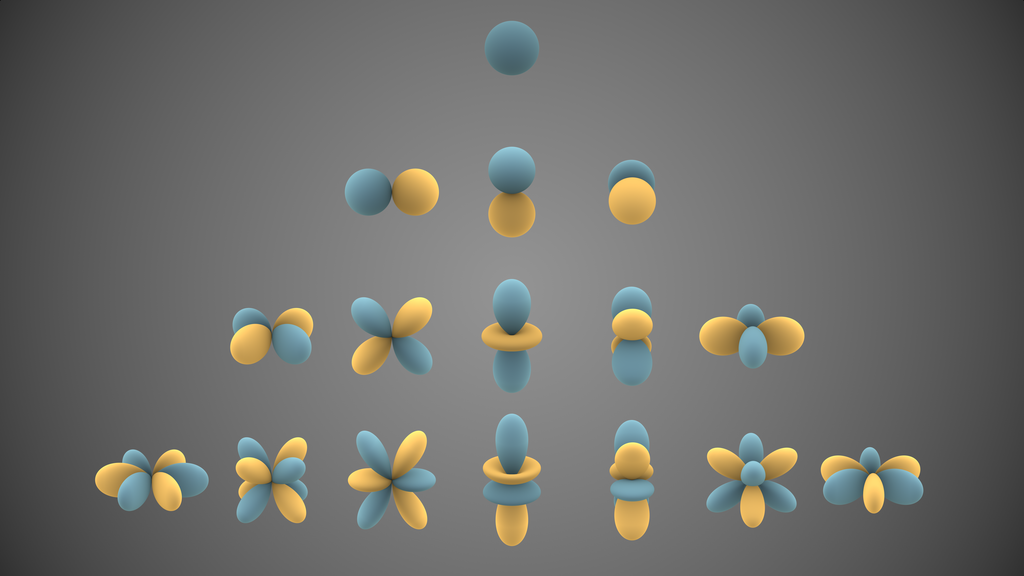
\includegraphics[width = 0.7\textwidth]{images/Spherical_Harmonics.png}
    \caption{Representation of the real component of the first few spherical harmonics models CITE.}
    \label{fig:SH}
\end{figure}

Most data reduction software in \ac{mx} use \ac{sh} as a basis for absorption correction calculations. This includes DIALS \cite{Winter2018}, the reduction software standardly used at Diamond Light Source.

Because empirical methods are independent of sample geometry, their efficiency depends on the number of symmetry equivalent reflections, which is limited by data multiplicity. Their applicability is therefore limited in low-symmetry space groups. More relevant to I23, empirical corrections become inadequate for modelling strong absorption effects above 3.5 Å, and an analytical correction is needed \cite{Kazantsev2021}.

%To analytically calculate the $A_{\hkl}$ factors in \cref{AbsFactor_allmaterials}, the shape and orientation have to be characterised in detail.
Characterising the shape and orientation in detail has previously been done using optical microscopy \cite{Leal2008, Strutz2011}. %(Leal 2008, Strutz 2011)
An alternative approach taken by I23 to obtain the 3D model is X-ray tomography, which has been applied to characterise and visualise crystals \cite{Merrifield2011, Warren2013}.%(Merrifield 2011, Warren 2013)

 It has previously been reported that using tomographic reconstructions and segmentation as a basis for absorption correction allows for the calculation of X-ray path lengths through all the different materials in the sample \cite{Brockhauser2008}. This tomography-based approach to corrections is the focus of this project.

\begin{figure}
    \centering
    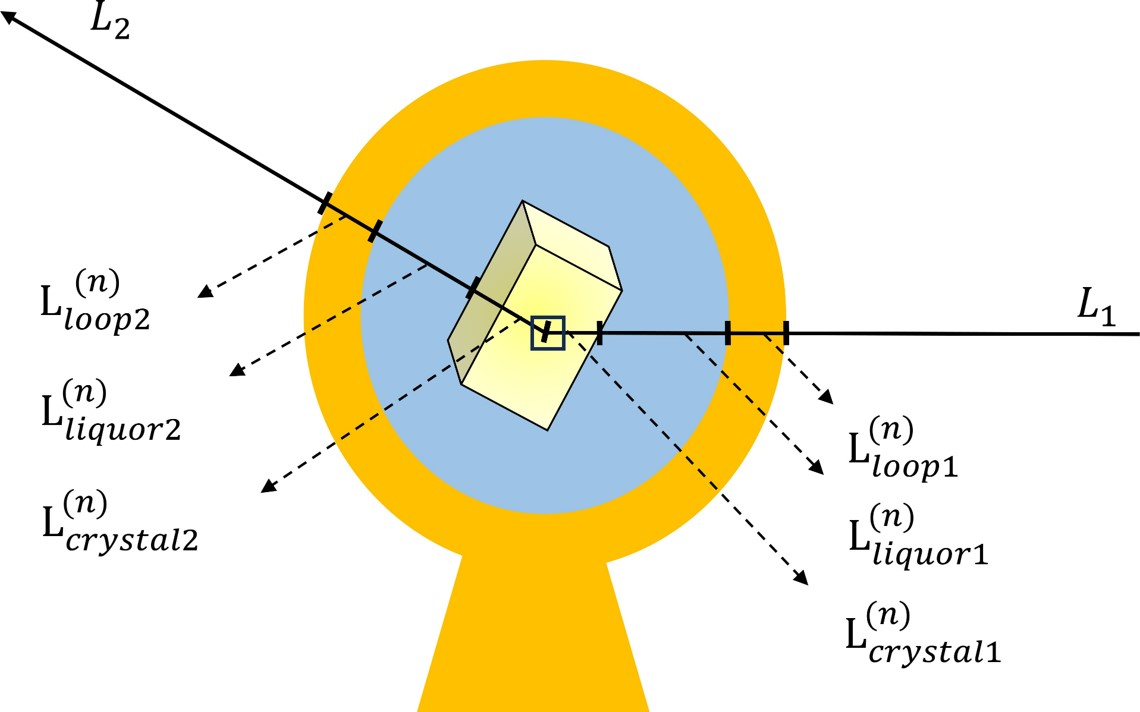
\includegraphics[width = 0.6\textwidth]{images/absorption correction diagram.jpg}
    \caption{Sketch illustrating the ray-tracing of absolute path lengths of X-rays through a sample, serving as the basis for analytically calculating absorption coefficients. $L_{m1}^{(n)}$ and $L_{m2}^{(n)}$ represent the path lengths of the incident and diffracted beams respectively for a material $m$. Adapted by Lu \textit{et al.} \cite{Lu}.
    % Fig. 1. A sketch illustrating the ray-tracing method used to calculate an absorption correction factor for a crystal voxel n. L(n)_m1 and L(n)_m2 represent the path lengths of m1	m2 the incident and diffracted X-ray beams through the material m (loop, liquor and crystal).
    }
    \label{fig:analytical correction model}
\end{figure}

By operating a tomography camera integrated into the endstation, I23 applies \ac{aac} based on a physical model of the sample derived from X-ray tomography, while empirical ones based on \ac{sh} are performed in the post-refinement step. Most relevant to this project is an approach that combines these two methods, by applying an empirical correction to the reconstructed physical model of the sample. This method is referred to as an \ac{acsh} in the remainder of this work. %in this project

A second alternative correction technique, which is a newer but less established practice at I23, is laser-shaping. By operating a femtosecond laser optimised for in-cryo crystallography samples, I23 uses laser-shaping to remove the non-diffracting material of a sample, leaving ideally only the diffracting material in a sample prior to the diffraction experiment. This thereby removes a significant amount of background noise, boosting the diffracting quality.

Previous studies have shown that both tomography-based reconstruction and laser-shaping can be beneficial for improving the detection of anomalous signal, but the effects of combining these practices has not yet been explored.

\subsection{Aims and Strategies}

The main aims of this project are as follows:

\begin{enumerate}
    \item Establish the AnACor software produces valid experimental absorption coefficients from X-ray tomography
    \item Demonstrate the successes and shortcomings of tomography-based \ac{aac} and that of a coupled approach (\ac{acsh}) to standard practices (\ac{sh})
    %\item Test the ability of the analytical approaches in identifying sodium ions in lysozyme protein
    \item Assess the effects of tomography-based analytical corrections on $f"$-refinement
    \item Assess the effects of laser-shaping as an alternative absorption correction \textit{in-situ} and with tomography-based analytical corrections
\end{enumerate}

\newpage
\section{Methodology}\label{sec:methodology}

All experiments concerning the data collection and processing were performed at the long-wavelength \ac{mx} beamline I23 at Diamond Light Source, UK. The data collection takes two experimental modes: X-ray diffraction and X-ray tomography. Data processing was also carried out at beamline facilities. %data from crystal samples at the I23 endstation.

\subsection{Diffraction and tomography data collection}

Experiments detailed in this project were collected on protein crystals of: thaumatin, thermolysin, insulin, and proteinase-K. Additional crystals listed in the appendix include chlorite dismutase (Cld) and OmpK36, which were collected on prior to the start of the project.
Sample preparation for in-vacuum data collection followed the standard procedure for I23 detailed by Duman \textit{et al.} (2021) \cite{Duman2021}.

The in-vacuum sample environment contains a cylindrical P12M detector as well as a multi-axis goniometer to enable collection  in multiple orientations; this provides access to high multiplicity and improves data completeness \cite{Finke2016}. The main axis of orientation is \textit{omega} ($\omega$), and the goniometer also has a \textit{kappa} ($\kappa$) and \textit{phi} ($\phi$) angle for re-orientation of crystals. %(illustrated PICTURE)

Each diffraction experiment collected multiple sweeps of 360$\degree$ of data, \textit{i.e.}, a full set of data. The diffraction data was automatically integrated with DIALS \cite{Winter2018} which provides the raw intensities, incident vectors, scattering vectors, and goniometer angles.

Following a diffraction experiment, the sample is kept in its in-beam position to immediately start tomography data collection. The order of the experiments is important because radiation damage will affect the higher resolution information first. The assembly for diffraction experiments is shown in the picture of the inside of the vacuum vessel in \cref{fig:vacuum_chamber}, with the position of the system for tomography data collection
shown with dotted lines (D) \cite{Kazantsev2021}.% A tomography camera is integrated into the sample environment to allow for a simple transition between the experimental modes \cite{Kazantsev2021}, as seen in \cref{fig:vacuum_chamber}.

\begin{figure}
    \centering
    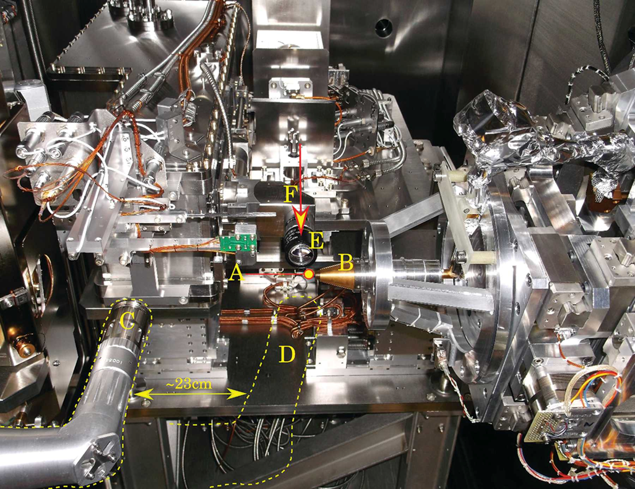
\includegraphics{images/tomo camera.png}
    \caption{A: Sample position; B: goniometer; C: tomography camera in retracted position; D: tomography camera in-beam position; E: viewing system; F: X-ray beam direction. Reproduced by Kazantsev \textit{et al.} (2021) \cite{Kazantsev2021}.}
    \label{fig:vacuum_chamber}
\end{figure}

Diffraction data collection requires the user to specify the energy, rotation increment, image time, and beam transmission. The number of datasets of one crystal corresponds to the diffraction experiments at the same energy using varying orientations of kappa and phi. The data collection parameters for each diffraction experiment on the aforementioned crystals are presented in \cref{diffration_table} in the appendix.

Tomography data collection also requires a specified energy, exposure time, rotation increment, and a range of $\omega$ angles to sweep. %While the energy of tomography scans used for the segmentation model does not need to match the experimental diffraction data they are used for, the projection images (also known as flat-fields) should be applied to a dataset with a matching energy. 
To ensure the matching of diffraction and tomography experiments, tomography is collected at every energy that diffraction is collected at, with $\kappa$ and $\phi$ set to zero. The tomography parameters used in these experiments are presented in \cref{tomo_table} in the appendix.

%Further information on the step-by-step procedure of tomography data collection at I23, as used in this work, is detailed in \href{https://confluence.diamond.ac.uk/x/h4HVDQ}{Tomography data collection instructions} on the Diamond Confluence page.

\subsection{Laser-shaping in cryo-crystallography}
% Unibody-Design fs laser
A peripheral lab at Diamond Light Source now houses a commercial femtosecond laser  that has been set up for laser-shaping crystal samples under cryogenic conditions. The product by Light Conversion is a \textbf{CARBIDE-CB5-6W} laser, with a tunable pulse duration between 190 \unit{fs} and 20 \unit{ps}, a maximum power output of 6 \unit{W}, and an air-cooled model. The laser is also installed with the \textbf{2H} \textit{HG for CARBIDE} harmonic generator model by Light Conversion, with output wavelength options of 1030, 515, and 343 \unit{nm}.%of 515 \unit{nm}, mounted on the laser head.
%https://lightcon.com/product/carbide-femtosecond-lasers/#cb5-specifications
%https://lightcon.com/product/harmonic-generator-for-carbide/#specifications

To allow for the swift transfer of samples from a liquid nitrogen bath directly to the liquid nitrogen-cooled goniometer at the femtosecond laser, the laser room used by I23 also houses \href{https://www.diamond.ac.uk/Home/Corporate-Literature/Annual-Review/Review2015/Villages/Macromolecular-Crystallography-Village/Macromolecular-Crystallography-Village-Developments/BART---the-new-robotic-sample-changer-for-MX-beamlines-at-Diamond.html}{BART}, a robotic sample changer for \ac{mx} beamlines at Diamond. The experimental setup allows for samples to be sustained at cryogenic temperatures during transfer and experiment.

\subsection{Data processing pipelines, DIALS, and AnACor}

Following collection, diffraction data was integrated with DIALS for scaling and merging. DIALS is one of the standard practice data integration softwares at Diamond Light Source using \ac{sh} to scale reflection data, produced in the form of an \textit{MTZ} file. The scaling and correction of reflections likewise produces merging statistics that provide information on the merged data quality.% $I/ \sigma$ and $R_{merge}$ values.

%Once the merging statistics have been obtained, the reflection data is also produced .
%Further experiments can be run with \href{http://ccp4.github.io/dimple}{Dimple}, an MX pipeline for structure refinement, provided there are anomalous scatterers in the crystal. Using the known \textit{pdb} file of the protein model with the reflection data in an \textit{mtz}, Dimple calculates anomalous density (Anode) peaks from atoms in the structure. The peak heights are affected by several factors, including structural isomerism, binding ions, and water molecules contained in the pdb. While they are not as reliable as merging statistics for assessing the reflection quality, they are used to generate high-resolution electron density maps, as seen in cref{}, which is imperative for MX structure determination.

%The alternative to DIALS in generating reflection data is taken using X-ray tomography, which is a longer, multi-step process as it currently entails manually reconstructing the sample model.

Tomography data can be visualised in \textit{ImageJ} \cite{Schroeder2020} or in \textit{DAWN} \cite{Basham2015}. After the completion of every tomography scan, the data is processed using the \textit{SAVU} pipeline \cite{Kazantsev2022}. The processing routine here first requires determination of the centre of rotation to align the tomography images; after this is a flat-field correction, followed by ring-artefact removal and reconstruction. Images are also cropped to remove as much background as possible. The flat-field-corrected images are an intermediate step in the reconstruction process. Examples of the flat-field-corrected images, raw projections, and flat-field corrected projections are presented in \cref{fig:tomo projections}. 

\begin{figure}
    \centering
    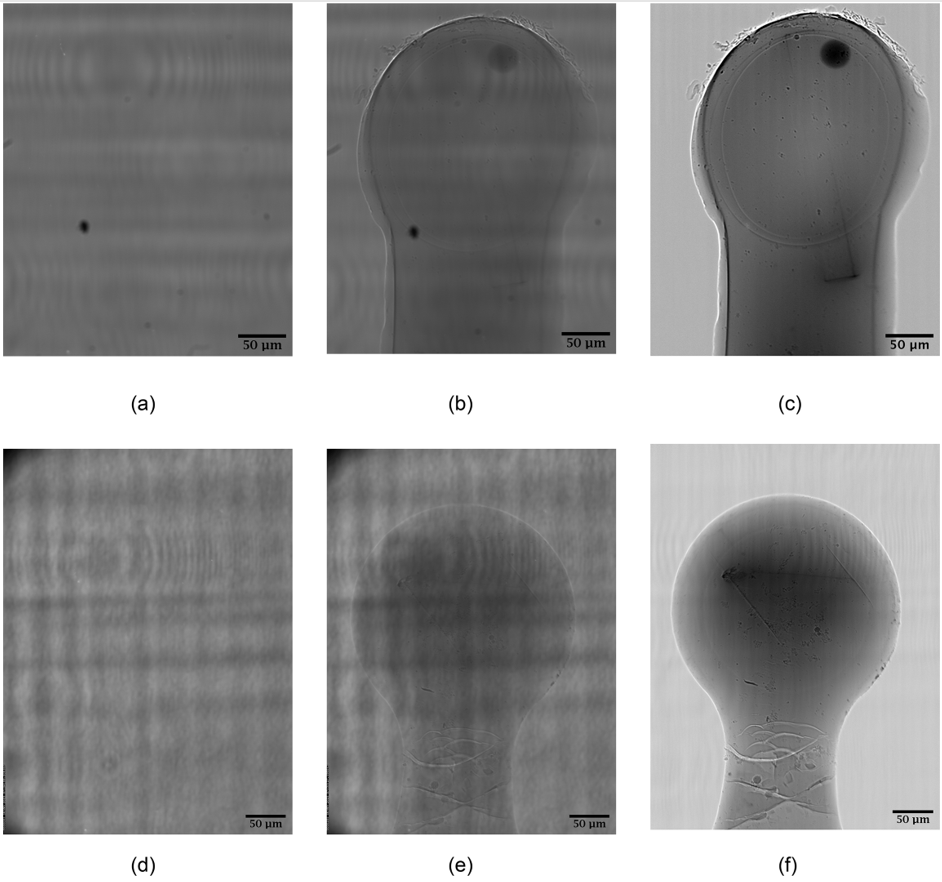
\includegraphics[width = 0.5\textwidth]{images/Tomo projection images CLD and Ompk high quality.png}
    \caption{Tomography projection images of Ompk (top row) and Cld (bottom row) showing: ((a) and (d)) background,  ((b) and (e)) sample, and ((c) and (f)) flat-field corrected images. Produced by Lu \textit{et al.} \cite{Lu2024}.}
    \label{fig:tomo projections}
\end{figure}

The final output from \textit{SAVU} provides reconstructed tomography slices (stacked along the long axis of the sample). Following this, the reconstructed images in the form of 32-bit two-dimensional \textit{tiff} files are converted to 8-bit data to reduce the data size. The reduced data is then imported and manually segmented in the visualisation software Avizo (Thermo Fisher) to distinguish between materials. The segmentation annotates every pixel in each tomography slice to a sample material or to the background, which in turn produces a detailed 3D sample model.

%\begin{figure}
    %\centering
    %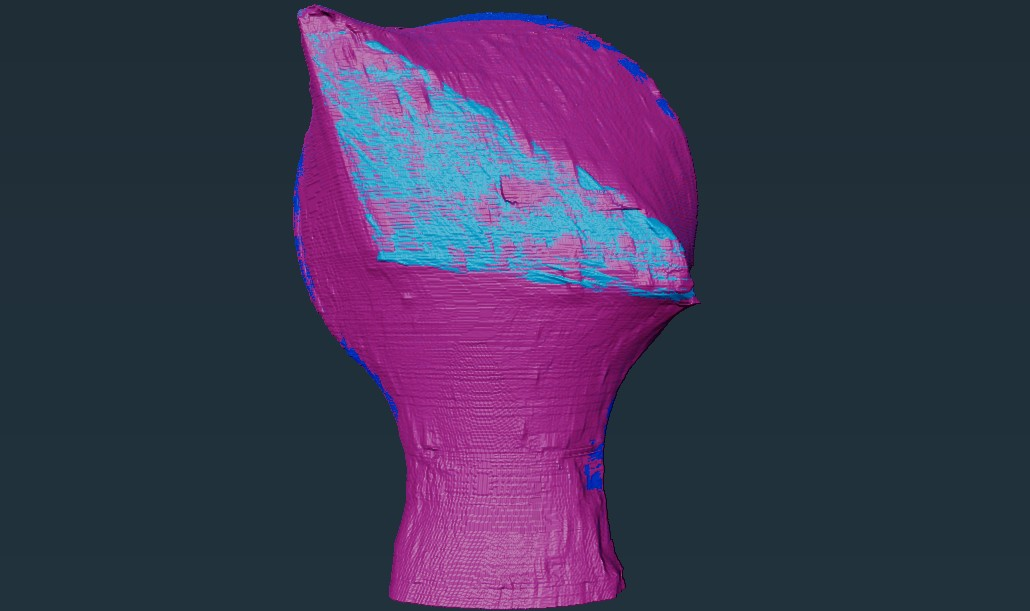
\includegraphics[width = 0.9\textwidth]{images/avizo_flats/cas3_1118.jpg}
    %\caption{3D-segmented model of cryopreserved sample of Cas3 crystal rendered in Avizo; the present materials are crystal (light blue), mother liquor (pink), sample mount (dark blue).}
    %\label{fig:Avizo}
%\end{figure}

The need for segmentation and for flat-field-corrected images comes in with AnACor, where the X-ray path lengths are traced through the 3D model to calculate absorption coefficients and determine the experimental absorption factors.
%, a ray-tracing software that has been developed collaboratively between I23, Graeme Winter at Diamond Light Source, and Yishun Lu at the Department of Engineering, University of Oxford. AnACor calculates the absorption factors for materials in an analytical 3D model with a discrete form of \cref{AbsFactor}, where the integral over crystal elements $dV$ is replaced with a sum over the crystal voxels $\Delta V$ from  reconstruction \cite{Lu2024}: %applies an analytical absorption correction strategy based on the 3D model of the sample derived from X-ray tomography.

%\begin{equation}
    %A_{\hkl} = \frac{1}{N} \sum_{n=1}^N A_{\hkl}^{(n)}
%\end{equation}
% which visualises provisional 3D models
This happens in two stages in AnACor: pre-processing and post-processing. In the pre-processing stage, the intensities from the flat-field-corrected images provided are mapped to the corresponding materials in the 3D-segmented model exported from Avizo. The mapping allows for the estimation of absorption coefficients for every material.%and the cropped flat-field images, and feeds these into AnACor to produce a threshold of the sample highlighting where it has high confidence in the presence of a certain percentage of each material. The outcome of pre-processing is a list of absorption factors that are based on where it believes 25\%, 50\%, 75\%, and 100\% of each material lies - this is known as the acceptance percentage. A lower acceptance percentage corresponds to higher confidence, and \textit{vice versa}. % acceptance of the presence

%Absorption factors used in the AnACor experiments were based on 50 \% acceptance of the material, unless stated otherwise.

In the post-processing stage, the absorption coefficients from the prior stage are used to calculate absorption factors, which are then applied to un-corrected reflections from the diffraction experiment. The post-processing step therefore requires the reflection data generated by DIALS. For this reason, the reflection data must be initially produced with DIALS. The output of this stage is the same as in DIALS; reflection data, with data statistics on merging quality - the difference to DIALS is that the two sets of reflection data produced by AnACor have been corrected analytically; one with \ac{sh} applied and one without.

Because pre-processing does not generate new reflection data and instead only calculates experimental absorption coefficients, the first stage of the software can also run on samples void of diffracting material, such as an empty loop or a loop containing solvent. The advantage of this is that samples containing only or largely one type of material will produce more reliable coefficients. The outputted values for the non-diffracting materials can then be used in the post-processing of another sample containing the same kind of solvent or loop, as well as the crystal.

Information on the AnACor ray-tracing algorithm applied to tomographic reconstructions is described in further detail in Lu \textit{et al.} \cite{Lu2024}.

Subsequent processing after obtaining reflection data is run with \href{http://ccp4.github.io/dimple}{\textit{Dimple}} \cite{Thorn2011}, an \ac{mx} pipeline for structure refinement, provided there are anomalous scatterers of interest in the crystal. The reflection data stored in \textit{MTZ} file format is mapped to a \ac{pdb} format modelling the atomic coordinates of the known protein, allowing for the calculation of anomalous density peaks from anomalous groups. The peak heights are affected by several factors, including structural isomerism, binding ions, and water molecules contained in the \ac{pdb}. %While the peaks are not as reliable as merging statistics for assessing the reflection quality, 
Dimple likewise generates anomalous difference Fourier maps, which are imperative for electron density maps and thus for \ac{mx} structure determination. %electron density maps, as seen in cref{}
%MTZ file format is used for the storage of reflection data

\begin{figure}[H]
    \centering
    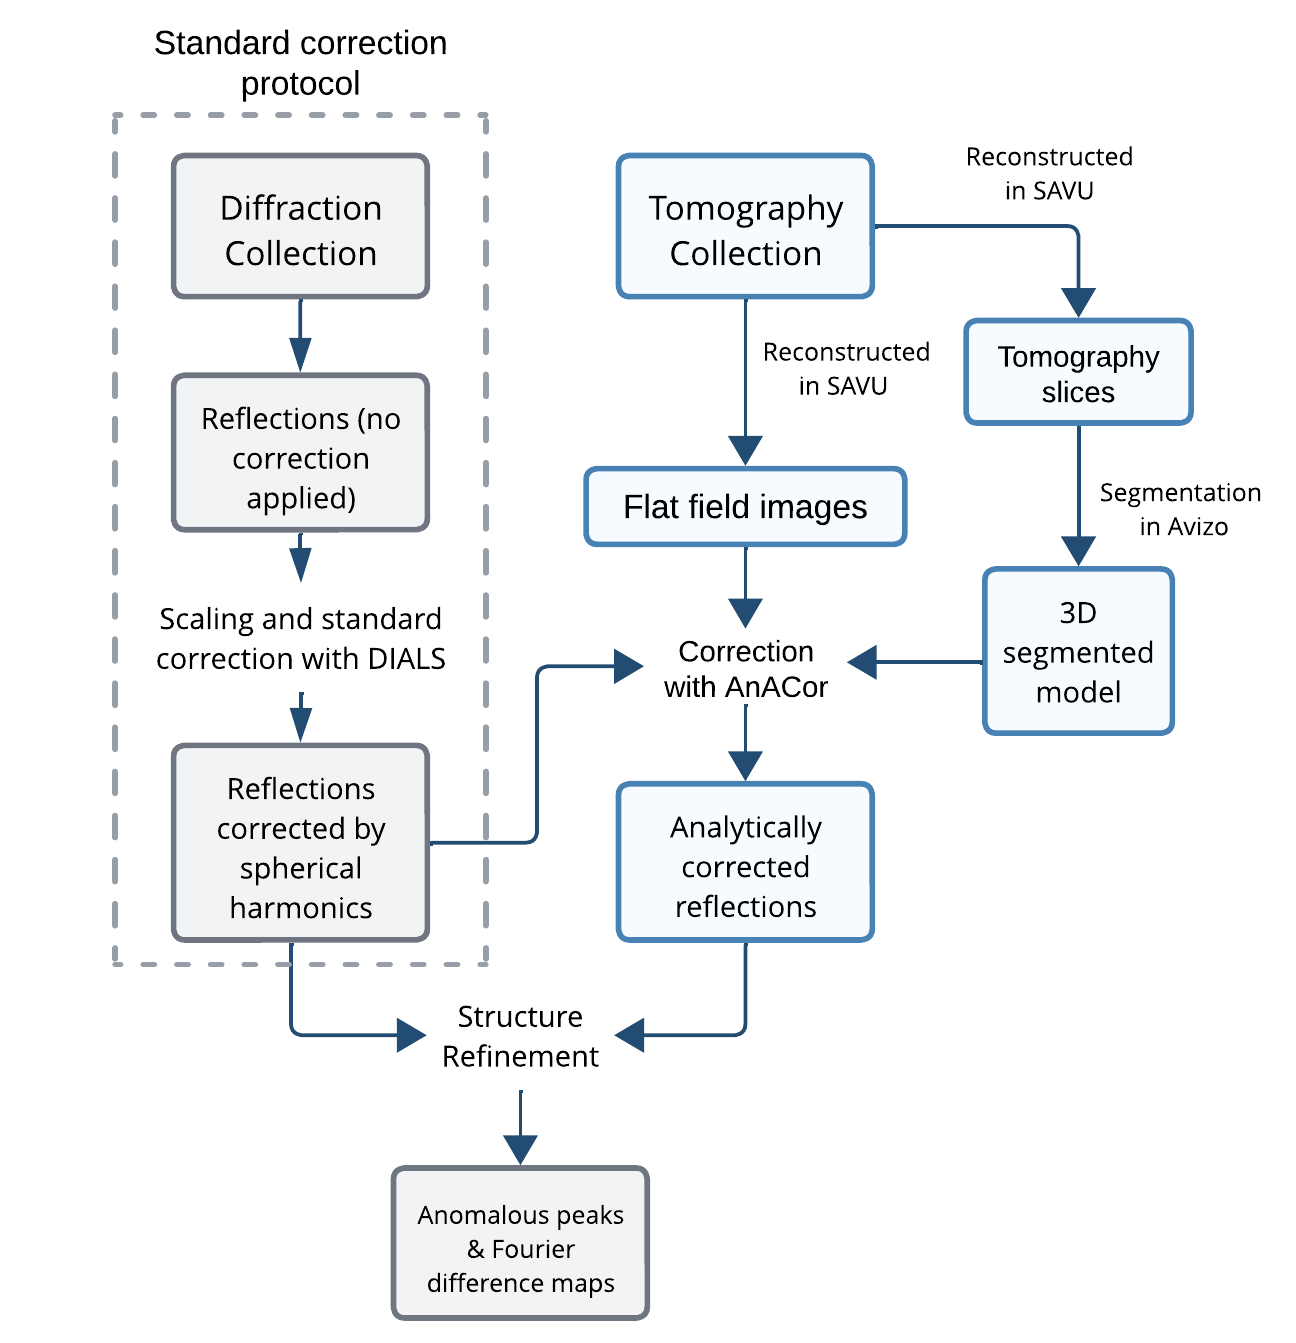
\includegraphics[width = 0.7\textwidth]{images/workflow.png}
    \caption{Current workflow of tomography data processing, highlighting the standard protocol for absorption correction using only DIALS, and the subsequent protocol needed for analytical corrections with AnACor.}
    \label{fig:workflow}
\end{figure}

The typical workflow for the data processing of tomography experiments, as well as the standard  protocol for absorption corrections, is presented in \cref{fig:workflow}. More information detailing the step-by-step procedure of this workflow, can be found on Diamond Confluence: \href{https://confluence.diamond.ac.uk/x/yIWuD}{Tomography data processing instructions}. %summarised in cref{}

\subsection{Phenix refinement for ion identification}%$f"$-

Phenix is a comprehensive software package for \ac{mx} structure determination that includes a software extension known as \textit{phenix.refine}. This platform allows for the refinement of various structural parameters, including the $f'$ and $f"$ for a given atom, based on the reflection data and \ac{pdb} structure provided. Given that absorption and emission are sensitive to both wavelength and to the molecular environment, the theoretical parameters are unique to every atom. By refining the model against the reflection data while keeping the theoretical $f'$ fixed, the experimental-calculated $f"$ can be used to identify the ion in question. This practice is still in development for the purpose of ion identification and is referred to as $f"$-refinement in this thesis.%and is used for ion identification at I23.

%As described in the methodology, t
The first stage of \textit{phenix.refine} uses the reflection data provided to produce a modified version of the molecular structure in \ac{pdb} format. This updated molecular structure is then used in the second stage with the same reflection data to estimate the theoretical $f'$ and $f"$ values of specified atoms that are believed to be in the structure. In the case of this experiment, $f'$ was fixed to its theoretical value for a given atom and energy, allowing for an experimental $f"$ to be refined over a specified number of cycles. This value is then corroborated with the theoretical value to determine whether the atom type can be correctly identified.% test the ability of identifying atoms of sulphur and zinc in the crystal by determining their $f"$ peak.

\subsection{Merging statistics: R factor, intensities and estimated uncertainties}

When reflection data is scaled, data reduction software such as DIALS also provide a range of statistical parameters, including completeness, multiplicity, and reflection intensities. In diffraction experiments, the data quality is usually assessed by the overall $R_{merge}$ factor based on the reflection intensities. The $R_{merge}$ is a measure of the average ratio of the spread of symmetry-equivalent reflection intensities to the estimated value of reflection intensity \cite{Dauter1999}:

\begin{equation}
    R_{merge} = \sum_{\hkl}\sum_i | I_{\hkl,i} - \langle I_{\hkl} \rangle | / \sum_{\hkl} \langle I_{\hkl} \rangle
\end{equation}

The value itself is calculated in different ways across different data reduction programmes. Due to its high dependence on data multiplicity, the $R$ factor is always higher for high-symmetry space groups compared to those in low symmetry. Higher multiplicity in turn leads to improved data quality, but this must also be weighed with the increase in the $R$ factor.

The merging of diffraction data naturally increases data multiplicity, which can be appealing for enhancing the quality of crystals of low-symmetry space groups with low multiplicity. As with any experiment, outliers can occur. This can be the result of incorrectly classified partially and fully recorded reflections. Merging equivalent intensities provides a chance to identify outliers and remove them from a diffraction experiment. This however must be done with a level of scrutiny and a physical reason for the rejection.

Complementary information about the data quality is provided by the ratio of intensities to their uncertainties:

\begin{equation}
    I / \sigma = \sum_{\hkl} I_{\hkl}/\sum_{\hkl} \sigma(I_{\hkl})
\end{equation}

Here, the $\sigma$ values are not trivially estimated and are usually computed in data reduction software packages. Correctly estimating intensity uncertainties is crucial for subsequent applications of the data, for instance in phasing, refinement, and the solving of anomalous-atom positions \cite{Dauter1999}.  

It was therefore in the interest of the following experiments to maximise the $I / \sigma$ values while minimising the $R_{merge}$ factors. These were the main parameters used in the assessment of data quality throughout this project.

Two other complementary indicators for assessing diffraction data quality are the resolution and completeness. The data completeness is defined by the number of reflections collected compared to the number of theoretically possible reflections for a given crystal symmetry \cite{Arkhipova2017}. %This could range from ...
Since each reflection contributes to the electron-density map, the completeness heavily determines the quality of maps \cite{Wlodawer2007}.



\section{Results and Discussion}

The scope of experiments in this project involve extensive use of AnACor, the prototype software used at beamline I23 for adding an analytical correction to reflections and reflection intensities \cite{Lu}. Previous work from I23 has documented the successes of tomographic reconstruction and segmentation pipelines to determine analytical absorption factors \cite{Kazantsev2021}; however, AnACor has only recently become the routine for this. The software is still in its developing stages with many reoccurring errors which limit our ability to do data processing and the reliability of results. Validation of the experimental results is therefore still necessary when possible.

One example of a step taken to improve reliability in this project is when samples containing solely the mother-liquor that crystals were grown in were available, tomography data would be collected on these as well as the crystal samples. The segmentation of loops containing only liquor allow for more reliable thresholds to be applied with fewer materials to account for, and therefore produces more accurate coefficients.

Since low-energy tomographic scans are prone to high contrast artefacts which limit visibility in the segmentation, tomography scans intended for diffraction experiments collected at or below 3 keV would be collected at 3.5 keV, in addition to the low energy. Distinguishing between materials in the 3.5 keV tomography scans is somewhat easier, and therefore provides better segmentation for the reflection data collected at lower energies.

%Finally ... preliminary tests

\subsection{Preliminary tests on AnACor}

Because the final reflection data heavily relies on the accuracy of absorption factors, the first experiments conducted for this project were a validation of the accuracy of AnACor's pre-process calculations. Theoretical absorption coefficients are given by the reciprocal of the attenuation length, which can be calculated for a specific material from its chemical formula, density, and the energy in question. The first experiment on AnACor used crystals of ethylene glycol and santovac to compare experimentally calculated coefficients from the software with theoretical coefficients.

The experimental coefficients of santovac, published in \cref{santovac_table}, are within 1.5 \% of the theoretical value for energies between 3 and 4.5 keV. This difference, however, appears to grow with energy, with a nearly 7\% difference at 6 keV. A similar trend is seen in \cref{ethylene_table} with the sudden jump from 1.2 \% at 5 keV to 6.3 \% at 6 keV for ethylene glycol.

Judging from the results of these two proteins alone, AnACor appears to overestimate coefficients at higher energies and similarly underestimates coefficients at lower energies. A possible explanation for the latter is the effect of high contrast at low energies limiting distinctions between materials; this however does not explain the overestimates at higher energies. It is also possible that the calculations do not sufficiently account for the changing dependence of absorption on wavelength, which is less strong at higher energies and would explain the the discrepancies.

A second validation experiment on AnACor involved samples of chlorite dismutase (Cld) and the membrane protein OmpK36 GD. Data on these two samples has already been analysed in Lu \textit{et al.} \cite{Lu} to compare the same approaches for absorption corrections discussed in this work: a \ac{sh} correction, analytical, and a combination of the two. The aim of this subsequent experiment, was to assess the accuracy of the absorption coefficients of crystal and liquor published in this paper. This was tested with the assumption that the accuracy would correlate to the best possible data quality, where the intensity to uncertainty ($I / \sigma$) peaks and the $R_{merge}$ factors are diminished.

Taking the coefficients published in this paper as a reference and varying both in intervals of \pm 10, sets up a variety of possible combinations of coefficient pairs which can together elucidate the optimal amount of variation in both for improving the merging statistics. The coefficients were varied from -20 \% to + 20 \%; after preliminary results were collected, the liquor coefficients were varied a further interval up to + 30 \%, giving a total of 30 possible coefficient variations. %The crystal reference was

The merging statics for all 30 AnACor experiments are shown in \cref{fig:cld_stats} for Cld and in \cref{fig:ompk_stats} for Ompk. The merging statistics of Cld tell a clearer story than that of Ompk: in \cref{fig:cld_stats} the $I/\sigma$ peaks between +10 and +20\% in the crystal factor, and +10\% for liquor; then looking at the R-factors, these values are minimised at the same variation. This indicates to the combination of coefficients that is presumably the most accurate for these materials, as it provides the best merging statistics.

While the differences in the maximum $I/\sigma$ and minimum R factors to their respective values at $\pm0,\pm0$ are small, in a perfect experiment these optimal statistics would align at $\pm0,\pm0$, as this would indicate that the references AnACor calculated are very good estimates. The underestimation here could be caused by several factors, including poor segmentation or insufficient threshold selections in pre-processing. Nonetheless, this procedure is still useful in correcting for small errors that deter AnACor from obtaining the true values. 

The Ompk results, shown in \cref{fig:ompk_stats}, are less clear by comparison. Despite the fact that there is an boundary where $I/\sigma$ is maximised, the R-factors do not change smoothly between experiments. Instead, there are only 3 values of the R-factor across all 30 runs with no incremental changes in between. This is a limitation in finding the optimal variation of coefficients, as the R-factor cannot be corroborated with the optimal $I/\sigma$.

%Establishing X-ray tomography as a valid approach: references for absorption correction calculations

%3D plots of finding the most optimal ACs for crystal and liquor using AnACor's AC values at 0.5 acceptance percentage as the reference

%This validation experiment ultimately took AC values calculated by AnACor in its pre-processing stage as a reference to run the post-processing of AnACor on a combination of AC of crystal and liquor varied in several increments from the reference. The aim of this was a check of AnACor's accuracy in determining the optimal AC that maximise the $I/ \sigma$ results while minimising the $R_{merge}$ factor.

In the interest of time, this validation check was not applied to the crystals investigated in the remainder of this project. Nonetheless, the experiment is a useful validation for finding the optimal absorption coefficients from AnACor for merging statistics. The scripts for this experiment have been complied to allow for users at I23 to apply this procedure to future tomography data. %A template of the scripts can be found at GitHub.


\subsection{Comparison of a spherical harmonics, analytical, and coupled approach} % empirical ?
% to absorption corrections
The primary focus of this project was to investigate the potential improvements in data quality by applying an analytical correction to diffraction data.
%Merging statistics and anomalous peak heights \cite{Lu}
In the interest of observing the effects of high absorption, crystal samples were largely collected at 3.0 and 3.5 keV, some of the lowest energies accessible to I23.

The first sample to be used for this investigation was a test crystal of thaumatin, collected at 3.0, 3.5, 4.0, and 4.5 keV. Because this early experiment was used primarily for segmentation practice, the results for the merging statistics can be found in the Appendix in \cref{fig:thaum1_stats}. Despite the segmentation being a rough model, the analytical approach already showed an improvement from \ac{sh}, with the two datasets at lower energies favouring \ac{acsh}, and the remaining datasets favouring \ac{aac}.

Subsequent tomography experiments were performed on two protein crystals of thermolysin. The first crystal, referred to as Thermolysin 1, was collected at three energies: 3.0, 3.5, and 3.8 keV, with datasets of varying orientations of $\kappa$ and $\phi$ at each energy, as listed in \cref{diffration_table}. The subsequent thermolysin crystal was collected only at 3.0 and 3.5 keV with the $\kappa$ and $\phi$ orientations also specified in \cref{diffration_table}.

\begin{figure}
    \centering
    \begin{tabular}{cc}
    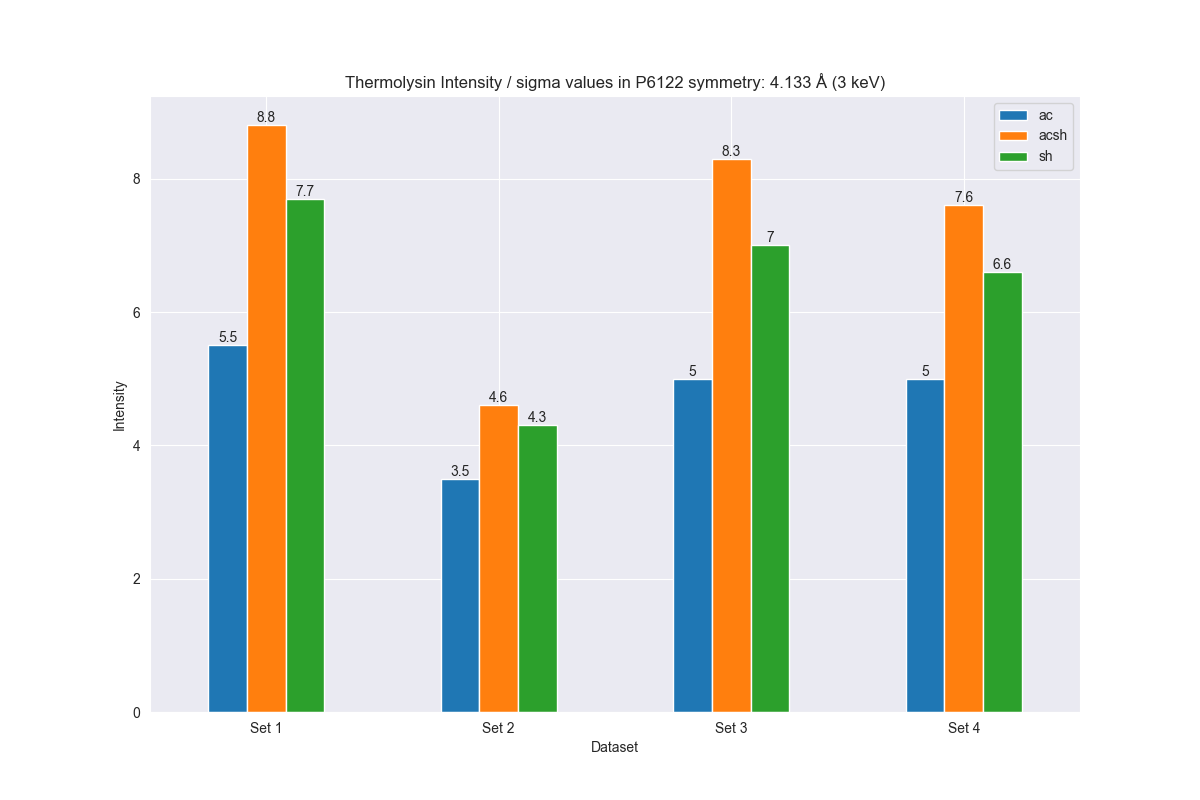
\includegraphics[width = 0.5\textwidth]{plots/exp1/tlys_9_P6122/3p0_I_over_sigma.png} & 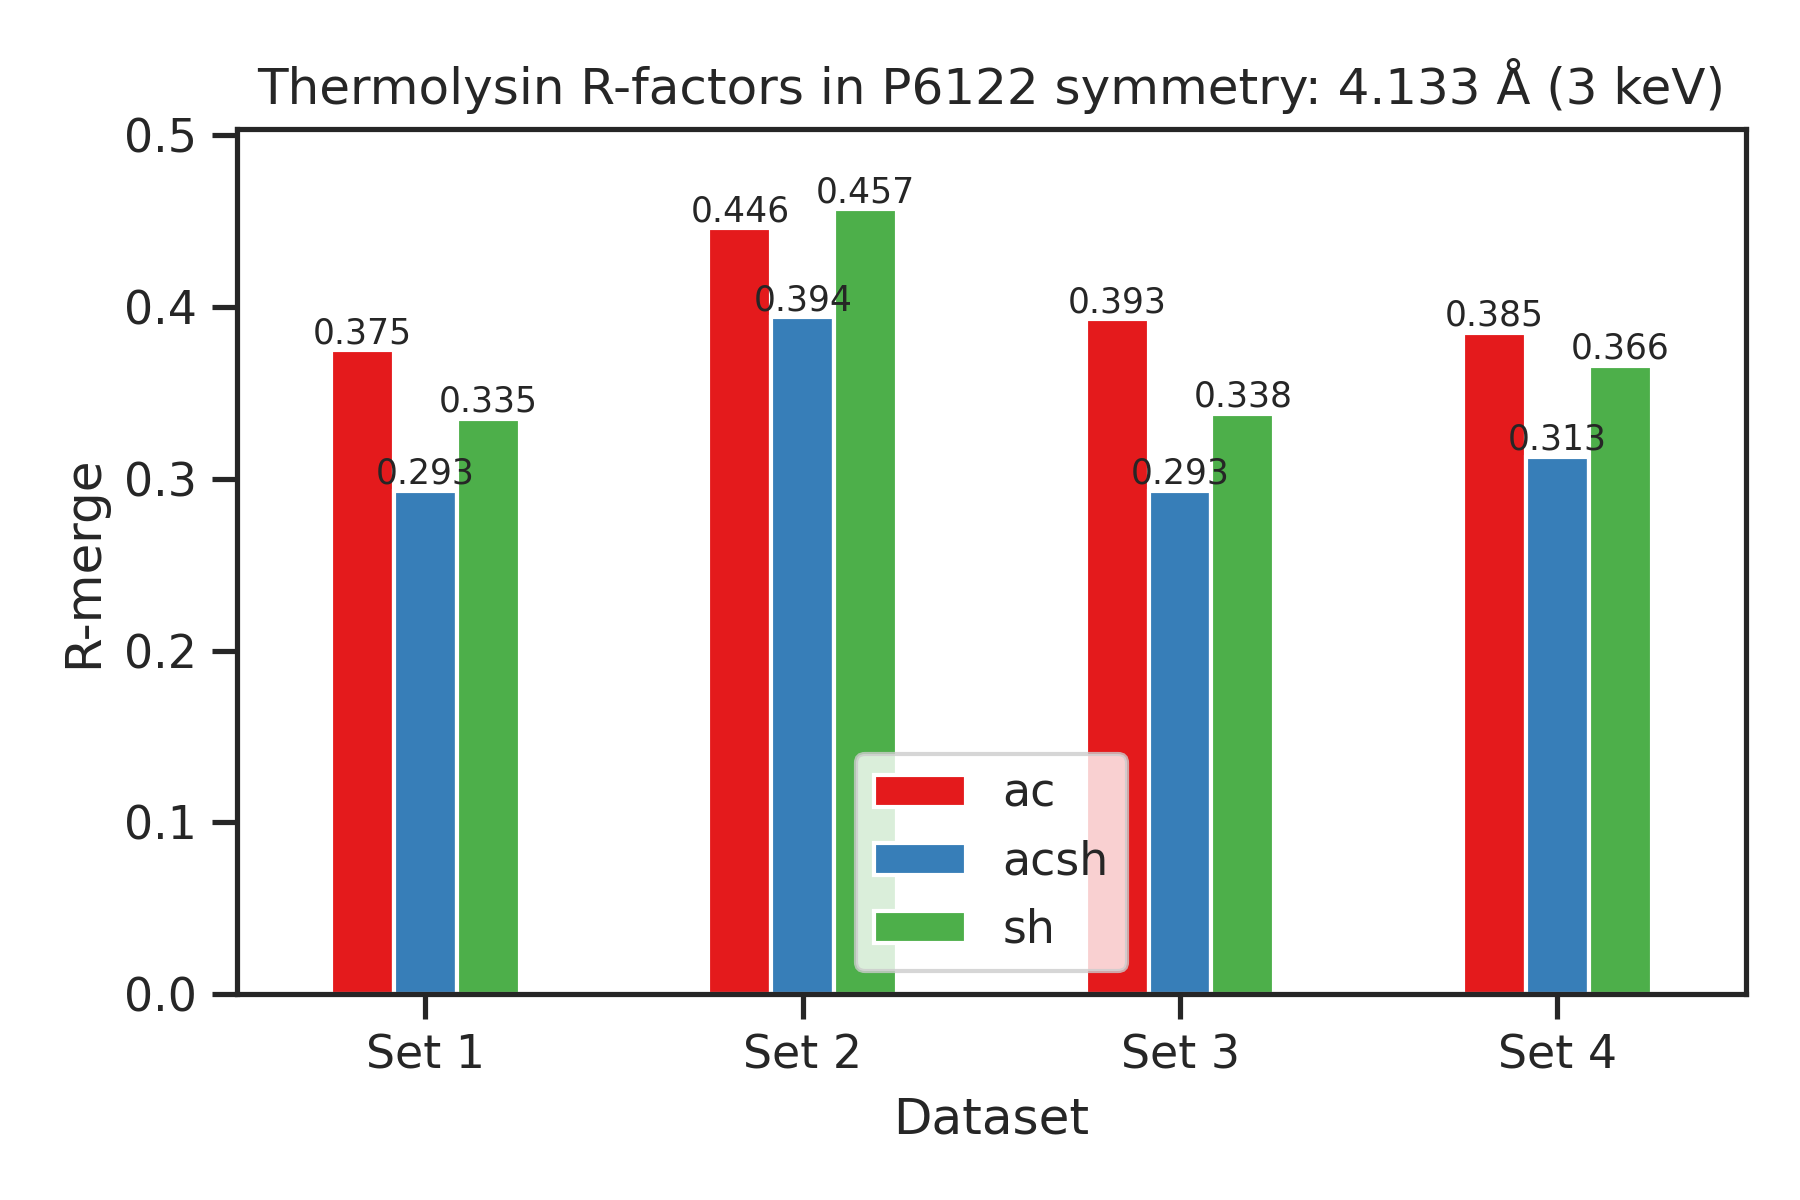
\includegraphics[width = 0.5\textwidth]{plots/exp1/tlys_9_P6122/3p0_rmerges.png}
    \end{tabular}
    \caption{Merging statistics for Thermolysin 1 at 3.0 keV.}
    \label{fig:tlys_9_3p0}
\end{figure}

\begin{figure}
    \centering
    \begin{tabular}{cc}
    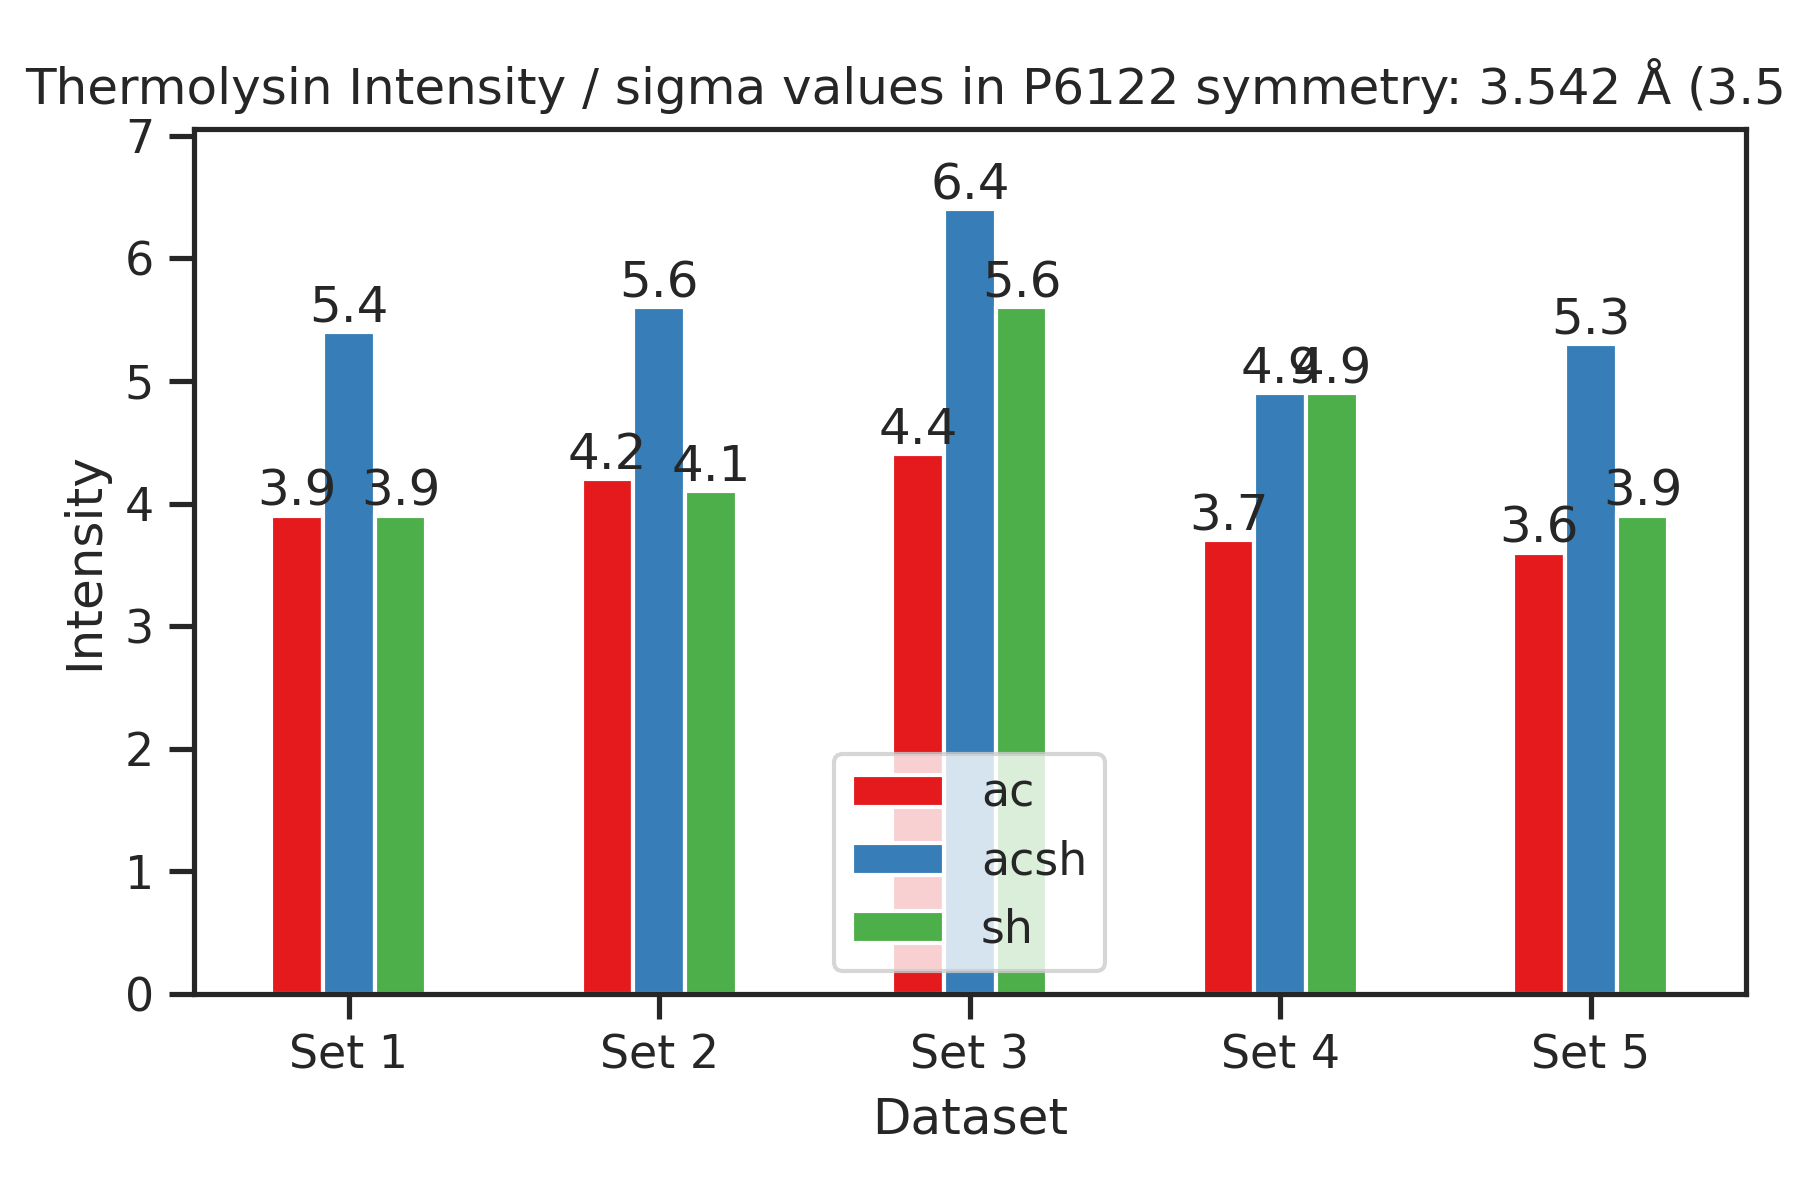
\includegraphics[width = 0.5\textwidth]{plots/exp1/tlys_9_P6122/3p5_I_over_sigma.png} & 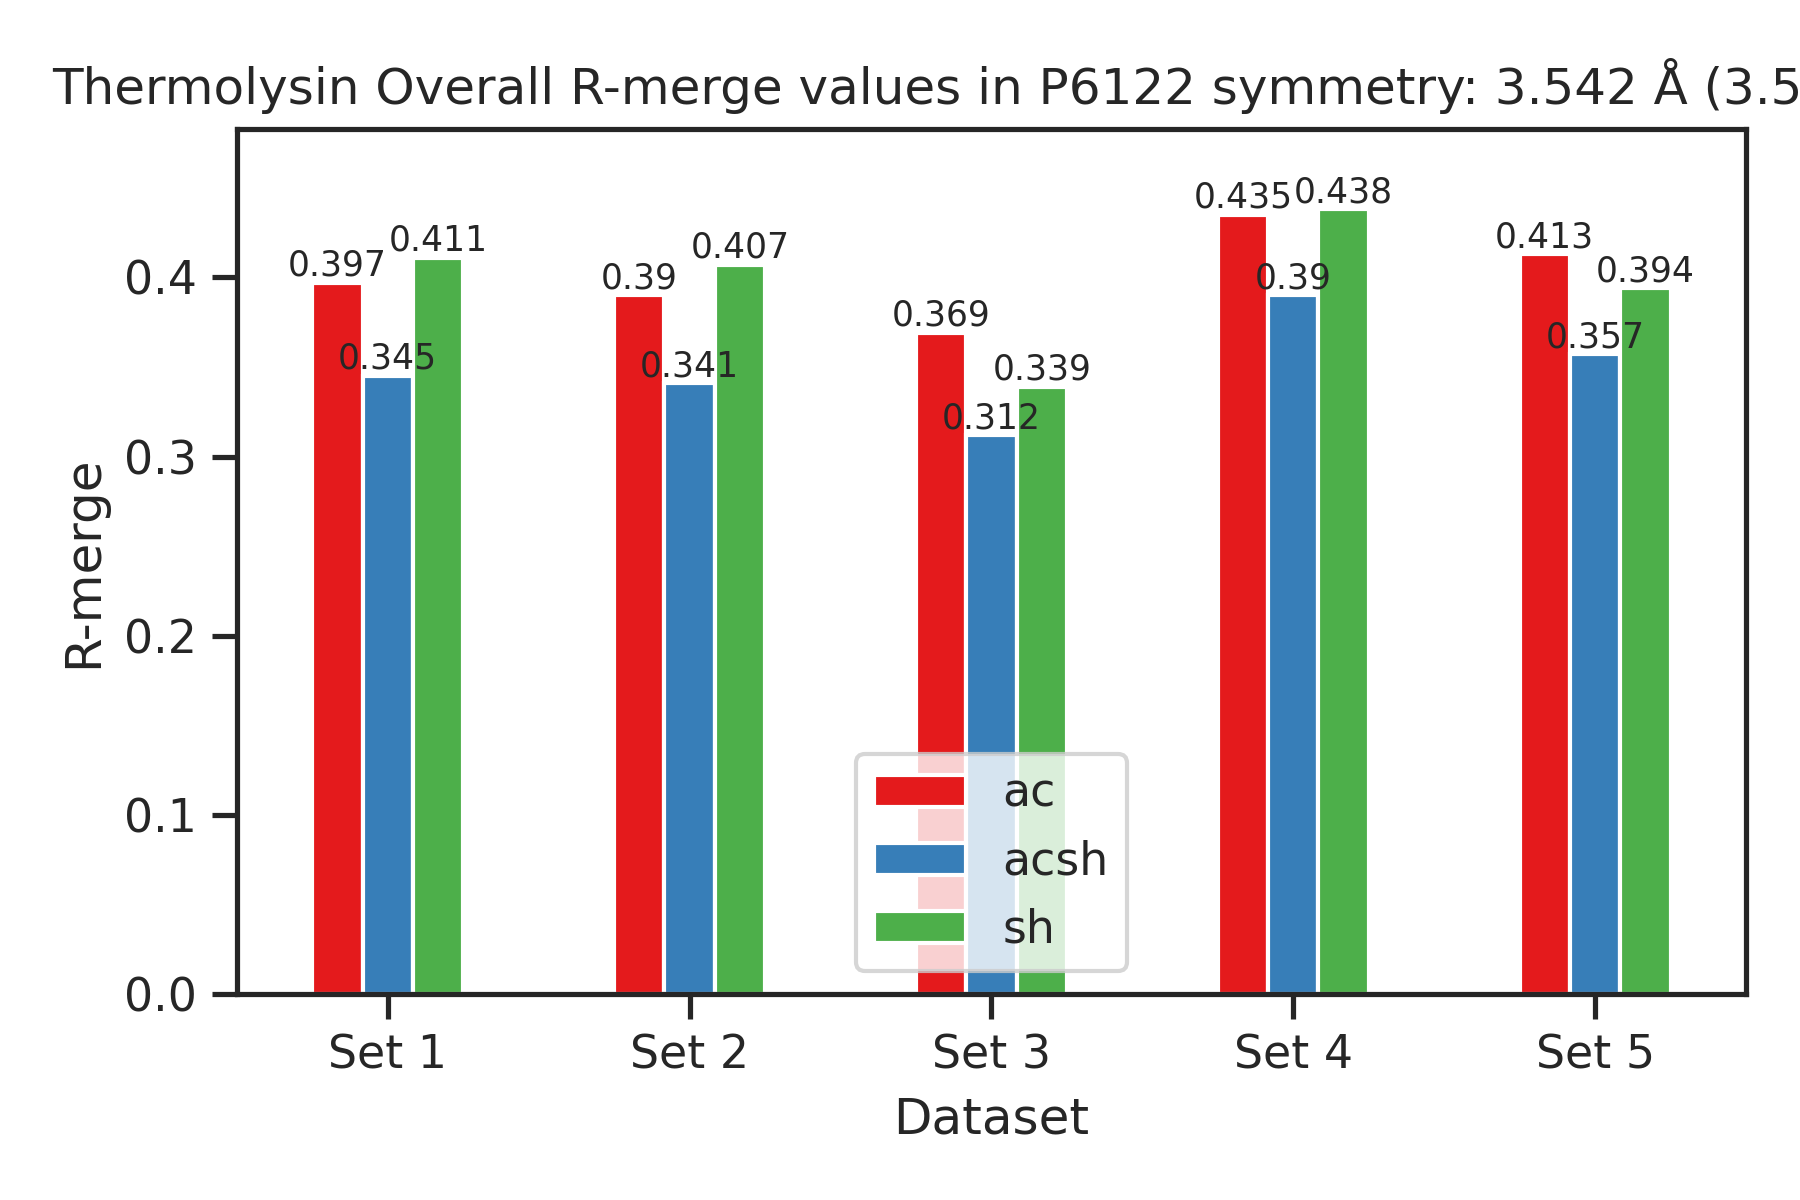
\includegraphics[width = 0.5\textwidth]{plots/exp1/tlys_9_P6122/3p5_rmerges.png}
    \end{tabular}
    \caption{Merging statistics for Thermolysin 1 at 3.5 keV.}
    \label{fig:tlys_9_3p5}
\end{figure}

\begin{figure}[h]
    \centering
    \begin{tabular}{cc}
    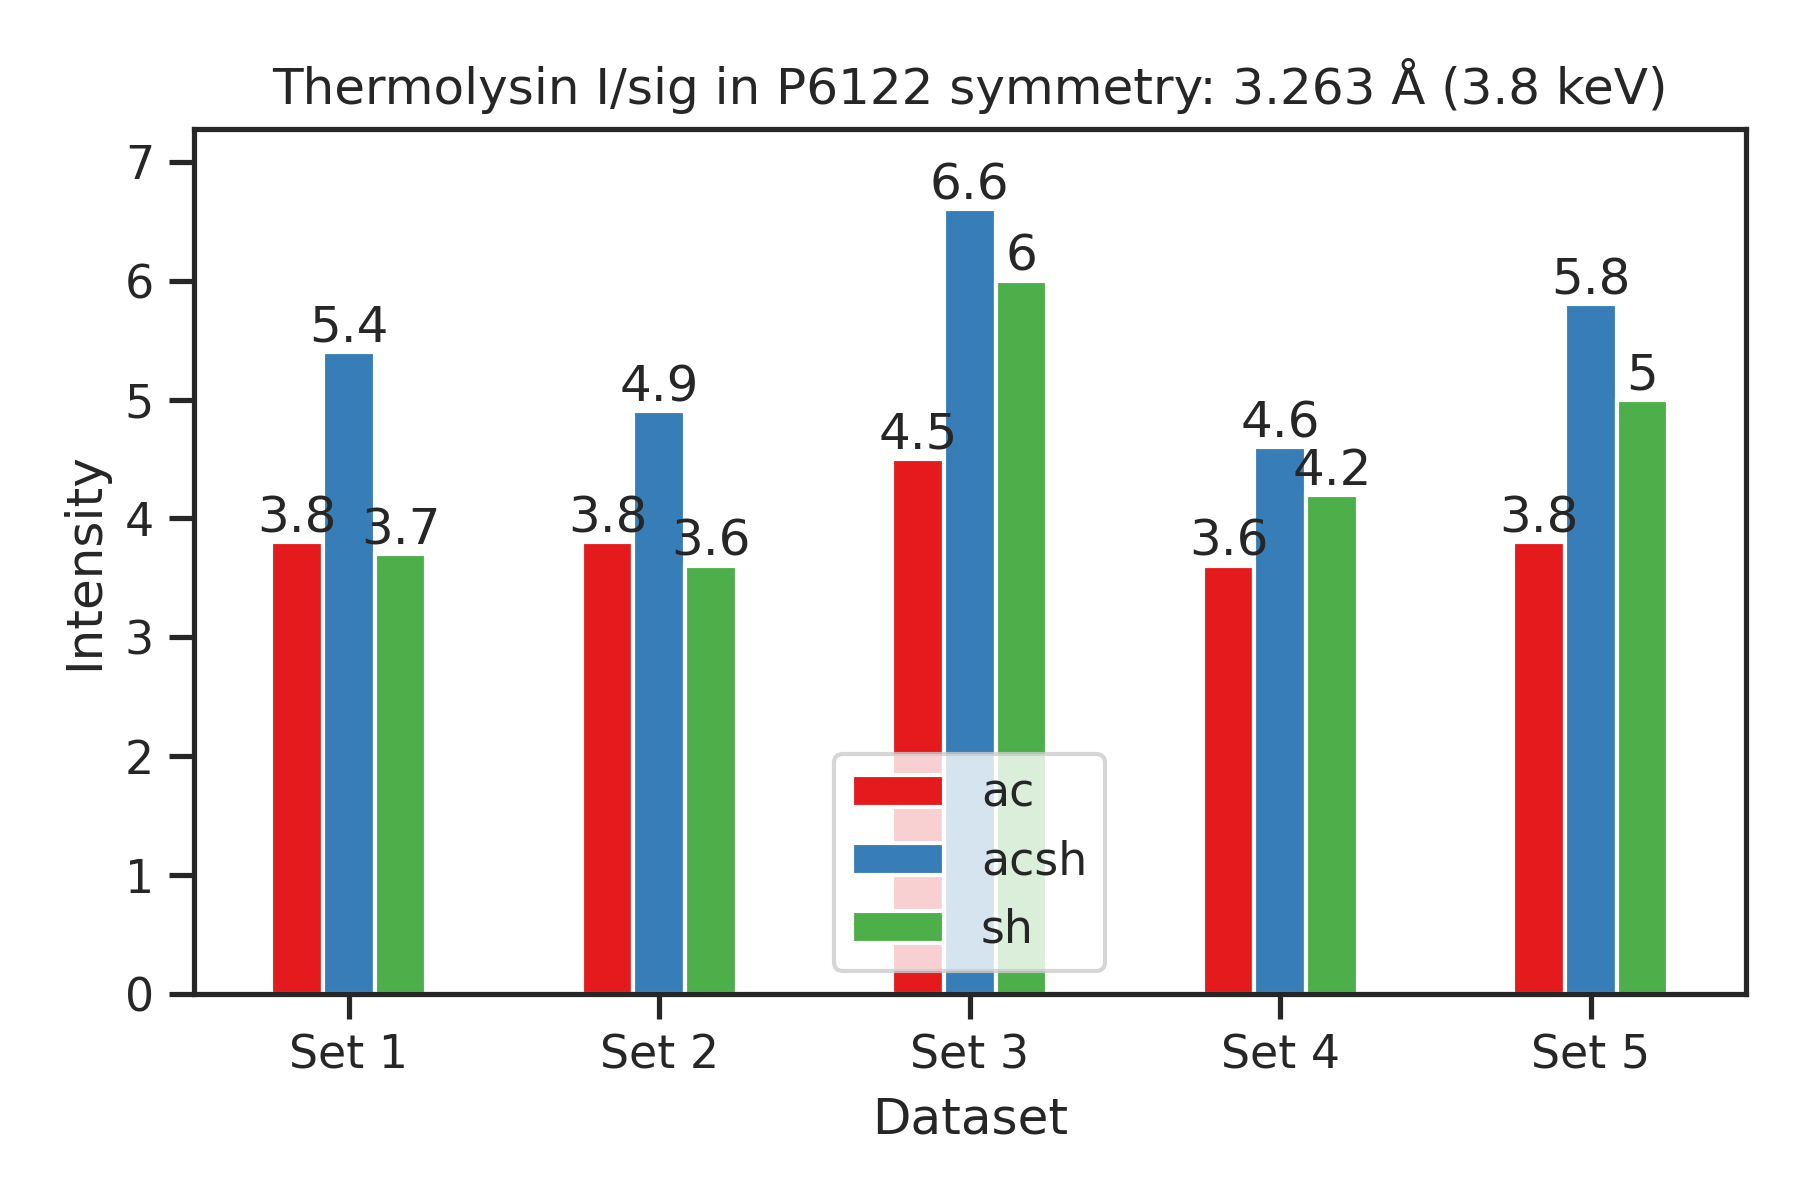
\includegraphics[width = 0.5\textwidth]{plots/exp1/tlys_9_P6122/3p8_I_over_sigma.png} & 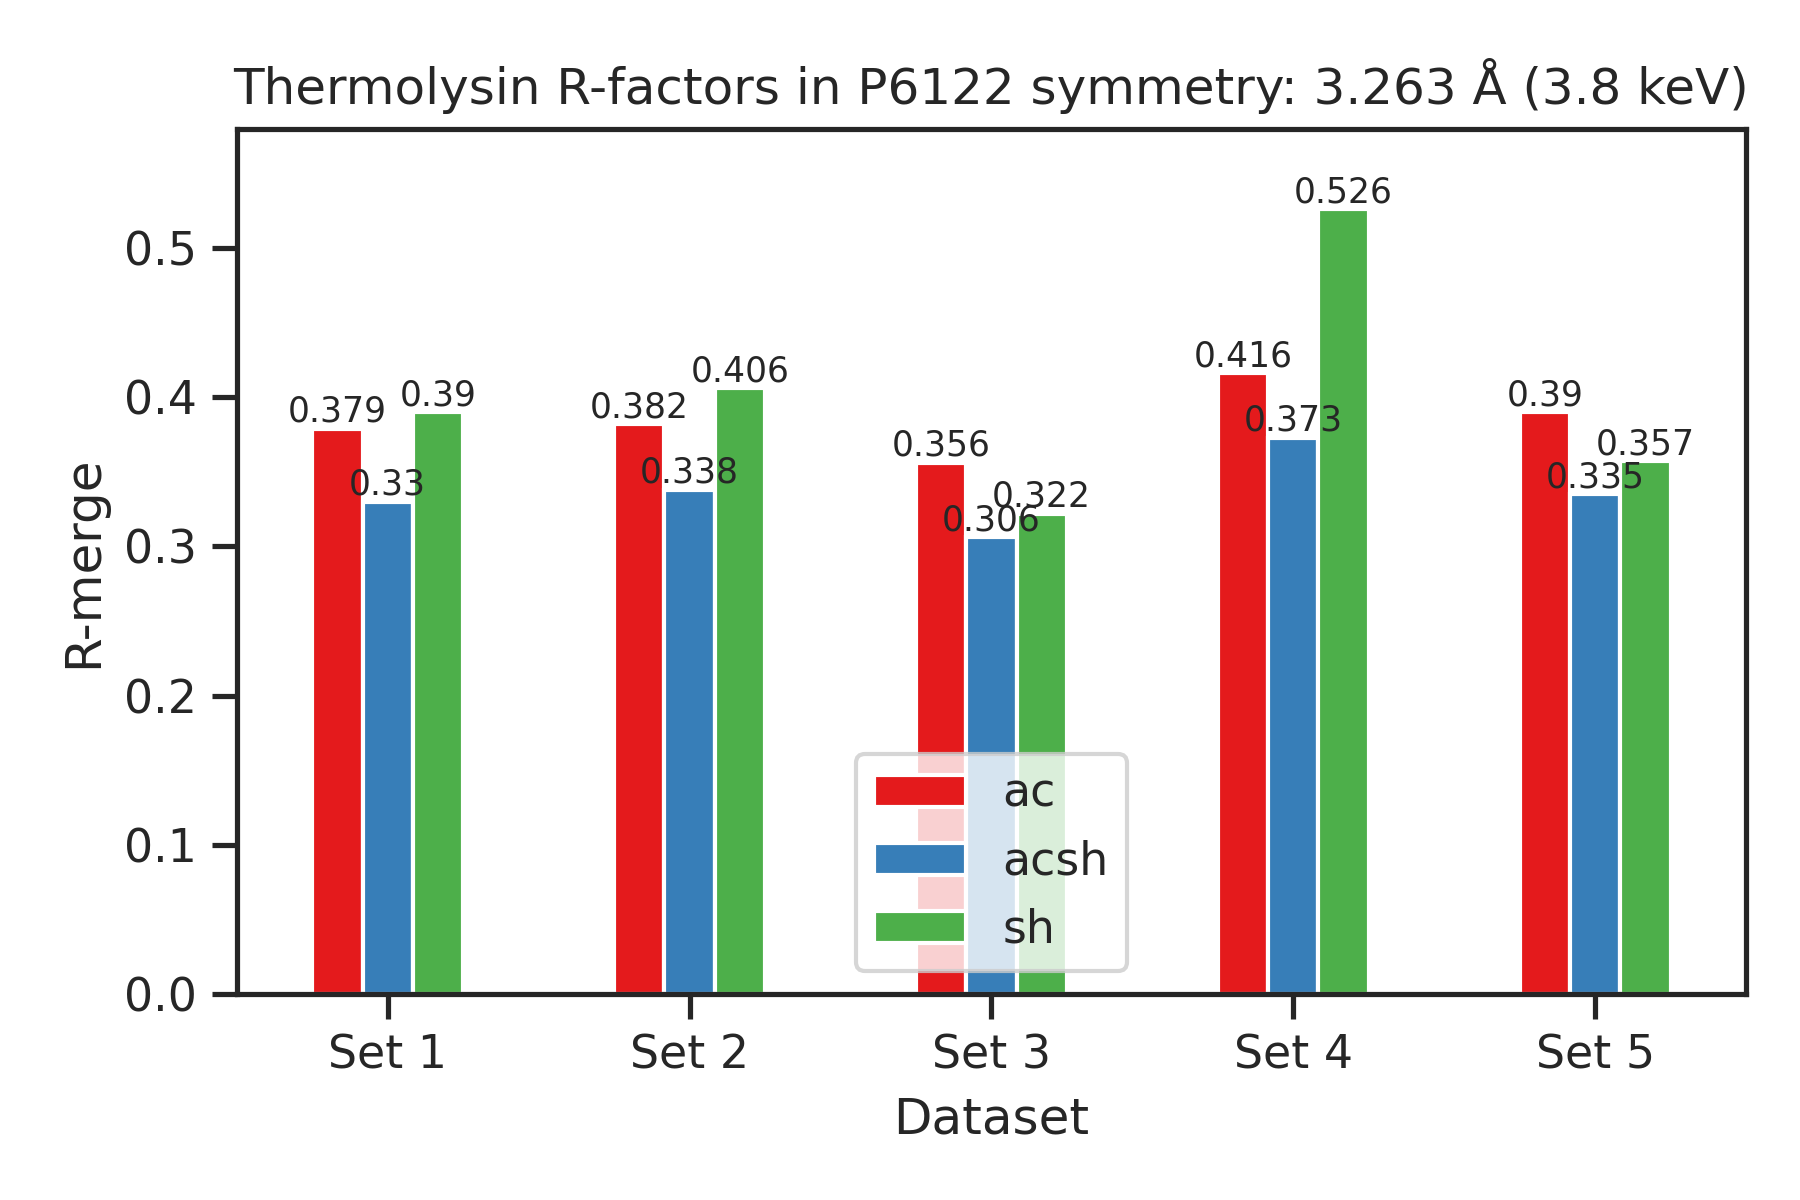
\includegraphics[width = 0.5\textwidth]{plots/exp1/tlys_9_P6122/3p8_rmerges.png}
    \end{tabular}
    \caption{Merging statistics for Thermolysin 1 at 3.8 keV.}
    \label{fig:tlys_9_3p8}
\end{figure}

Taking into account both the increase in $I/\sigma$ and decrease in $R_{merge}$, the merging statistics from Thermolysin 1 showed that \ac{acsh}, which combines tomography with spherical harmonics, was on average the best approach. While this was the case for every dataset of Thermolysin 1, some instances showed only a small improvement compared to \ac{sh}. Likewise, the standalone analytical approach was on average worse than \ac{sh} as well as \ac{acsh}.

Changes in energy are not expected to affect the reflection data in a relevant way; however, energies that were collected subsequently are expected to be more affected by radiation damage from longer exposure to the beam. If segmentation was then performed on a dataset collected early on in the tomography experiment, there can be discrepancies between the analytical model and a more-so radiation-damaged dataset.

%Following collection of reflection data, the AnACor results are used for structure refinement in Dimple, which generates anomalous density peaks for all the detected anomalous atoms and molecules based on the provided model. The results of Thermolysin 1

The merging statistics for Thermolysin 2, seen in \cref{fig:tlys_2_3p0} and \cref{fig:tlys_2_3p5} overwhelmingly show the same trend, with \ac{acsh} being the dominating correction method across all datasets and energies. This was corroborated with the $I/\sigma$ values and the R factors.
%that \ac{acsh} is once again the best correction method
%Results from Thermolysin 2 overwhelmingly show that \ac{acsh} is the dominating correction method, with $I/ \sigma$ highest and the R factors dipping across every dataset.

Thermolysin belongs to the symmetry space group \textit{P}6\textsubscript{1}22. While processing in \textit{P}6\textsubscript{1}22 is therefore needed for obtaining reflection information, high symmetry crystals can still be processed in low symmetry groups, such as \textit{P}\textsubscript{1}, to observe the general merging statistics of the experiment, independent of reflections.

\begin{figure}[h]
    \centering
    \begin{tabular}{cc}
    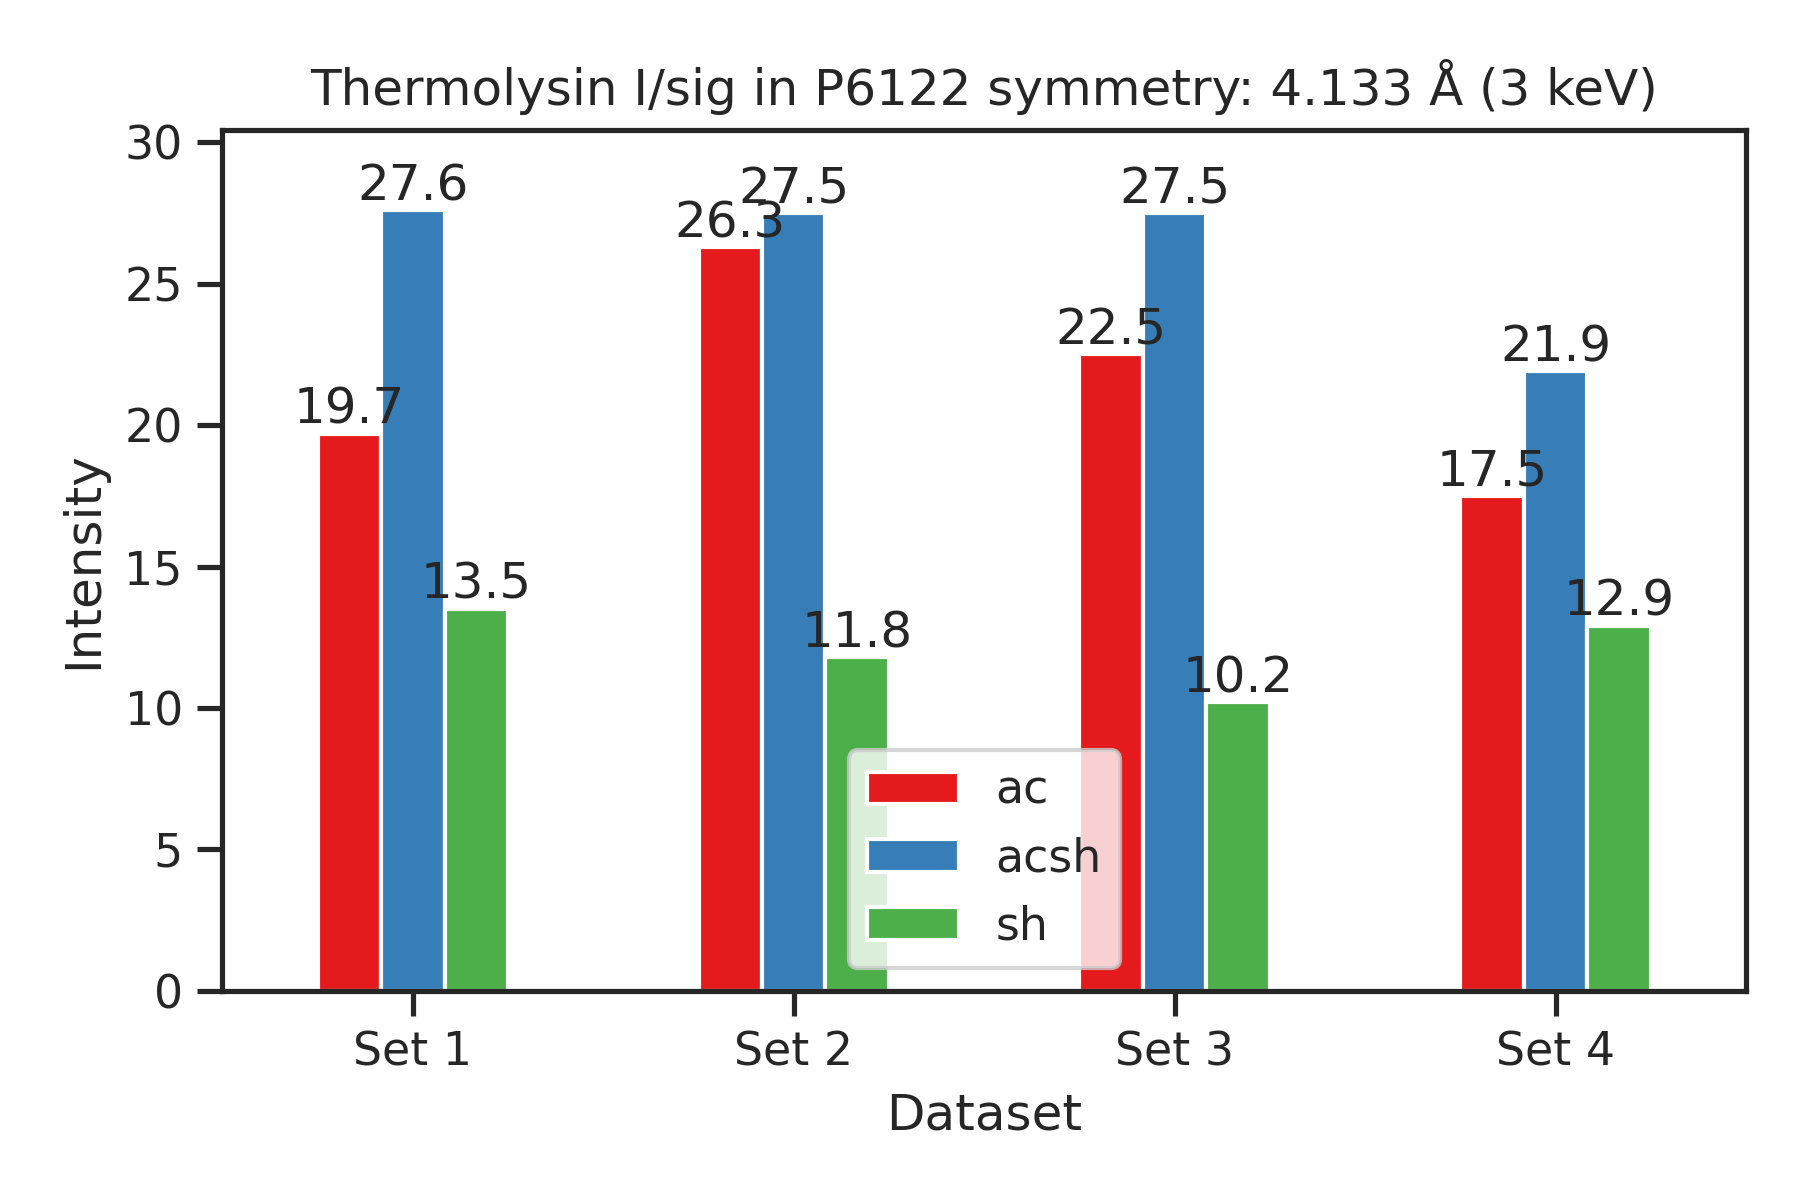
\includegraphics[width = 0.5\textwidth]{plots/exp1/tlys_2_P6122/3p0_I_over_sigma.png} & 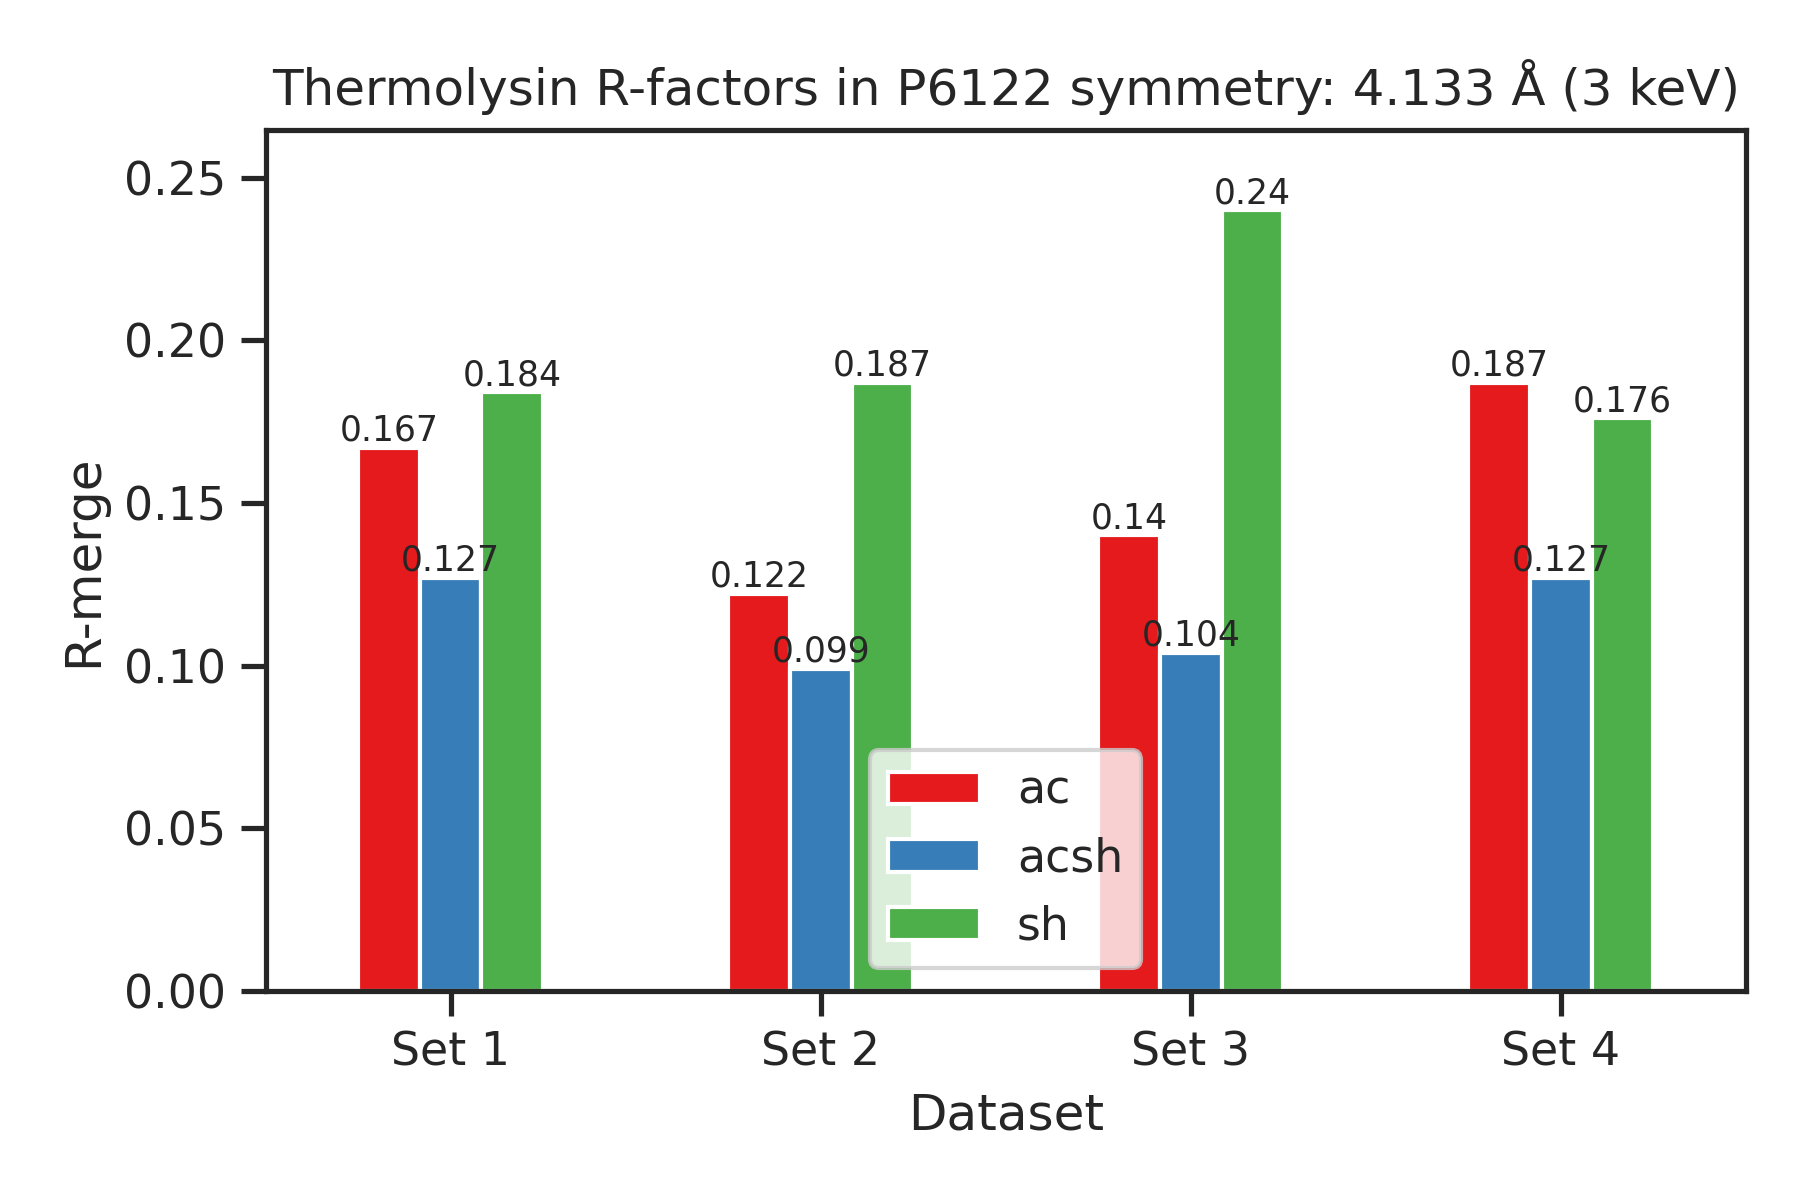
\includegraphics[width = 0.5\textwidth]{plots/exp1/tlys_2_P6122/3p0_rmerges.png}
    \end{tabular}
    \caption{Merging statistics for Thermolysin 2 at 3.0 keV.}
    \label{fig:tlys_2_3p0}
\end{figure}

\begin{figure}[h]
    \centering
    \begin{tabular}{cc}
    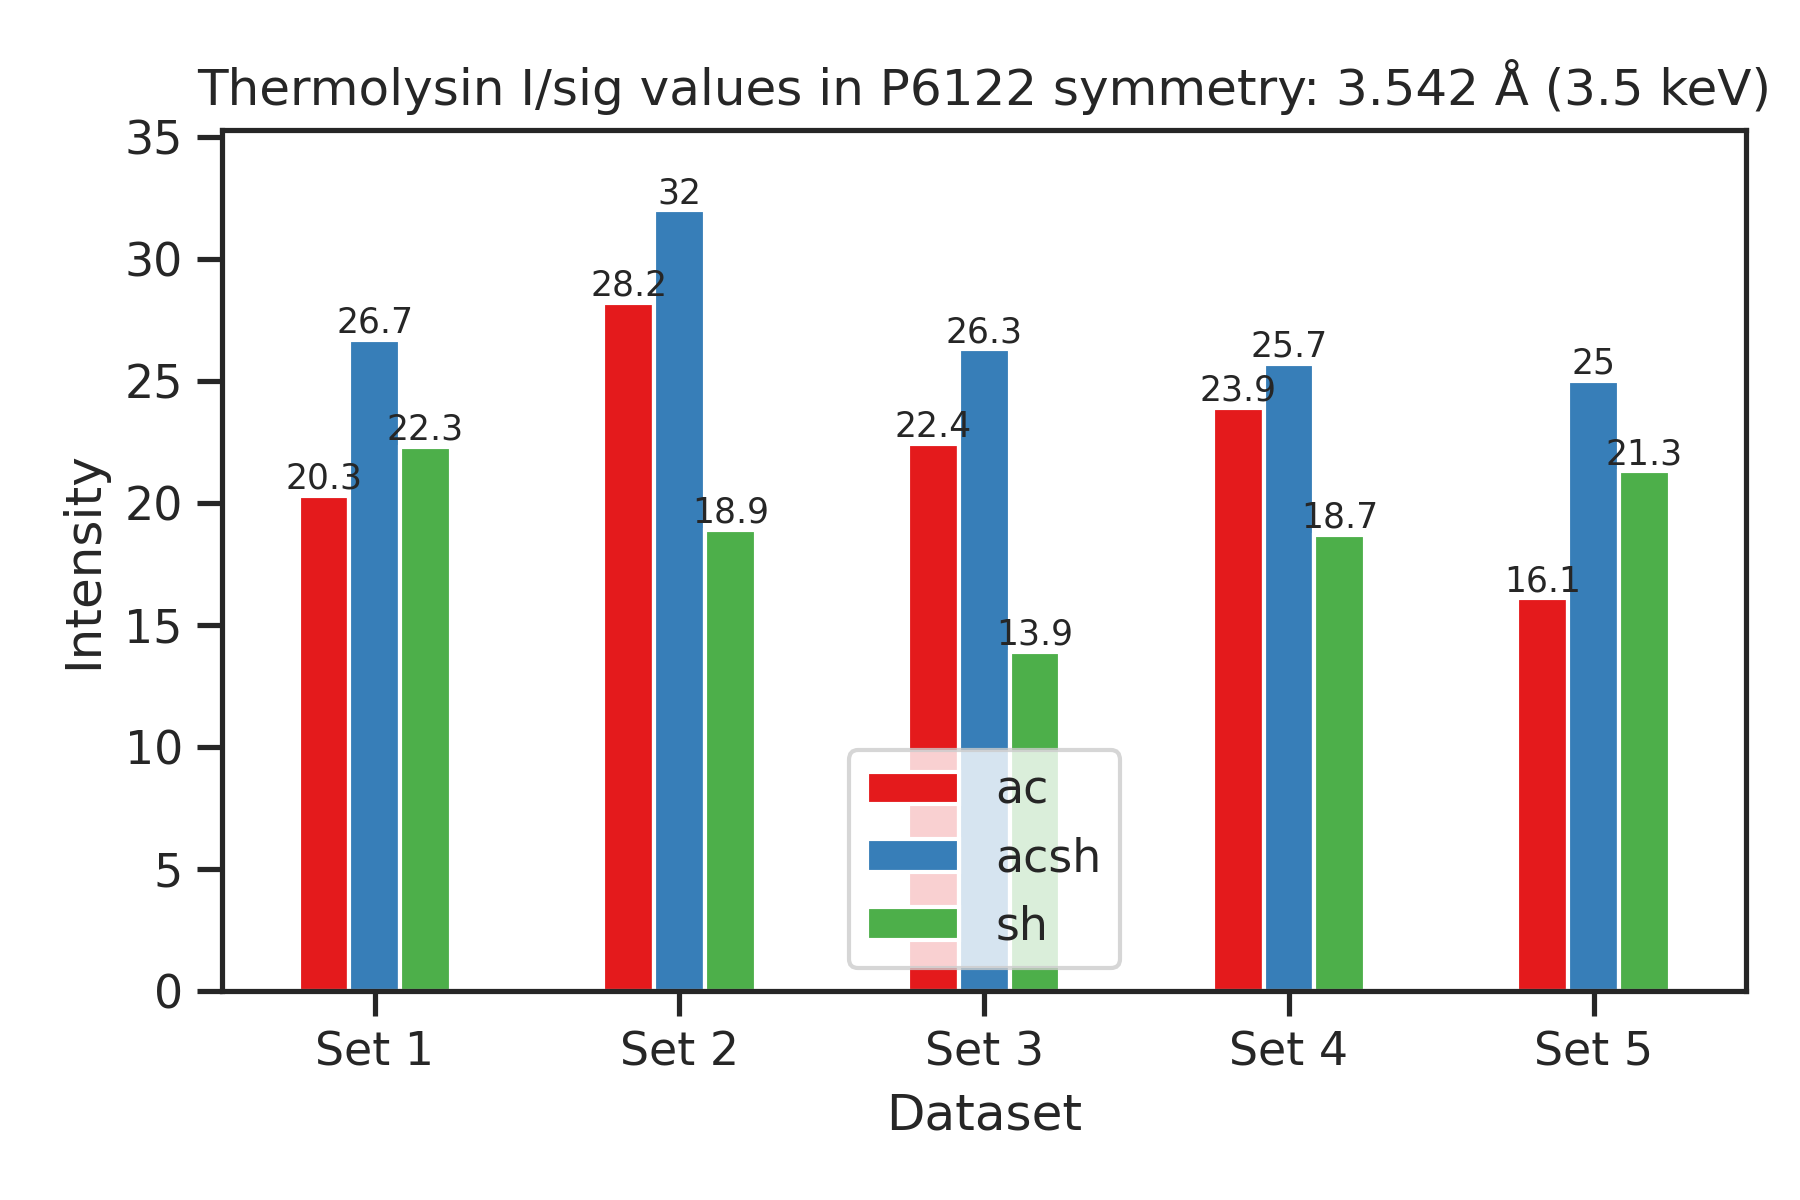
\includegraphics[width = 0.5\textwidth]{plots/exp1/tlys_2_P6122/3p5_I_over_sigma.png} & 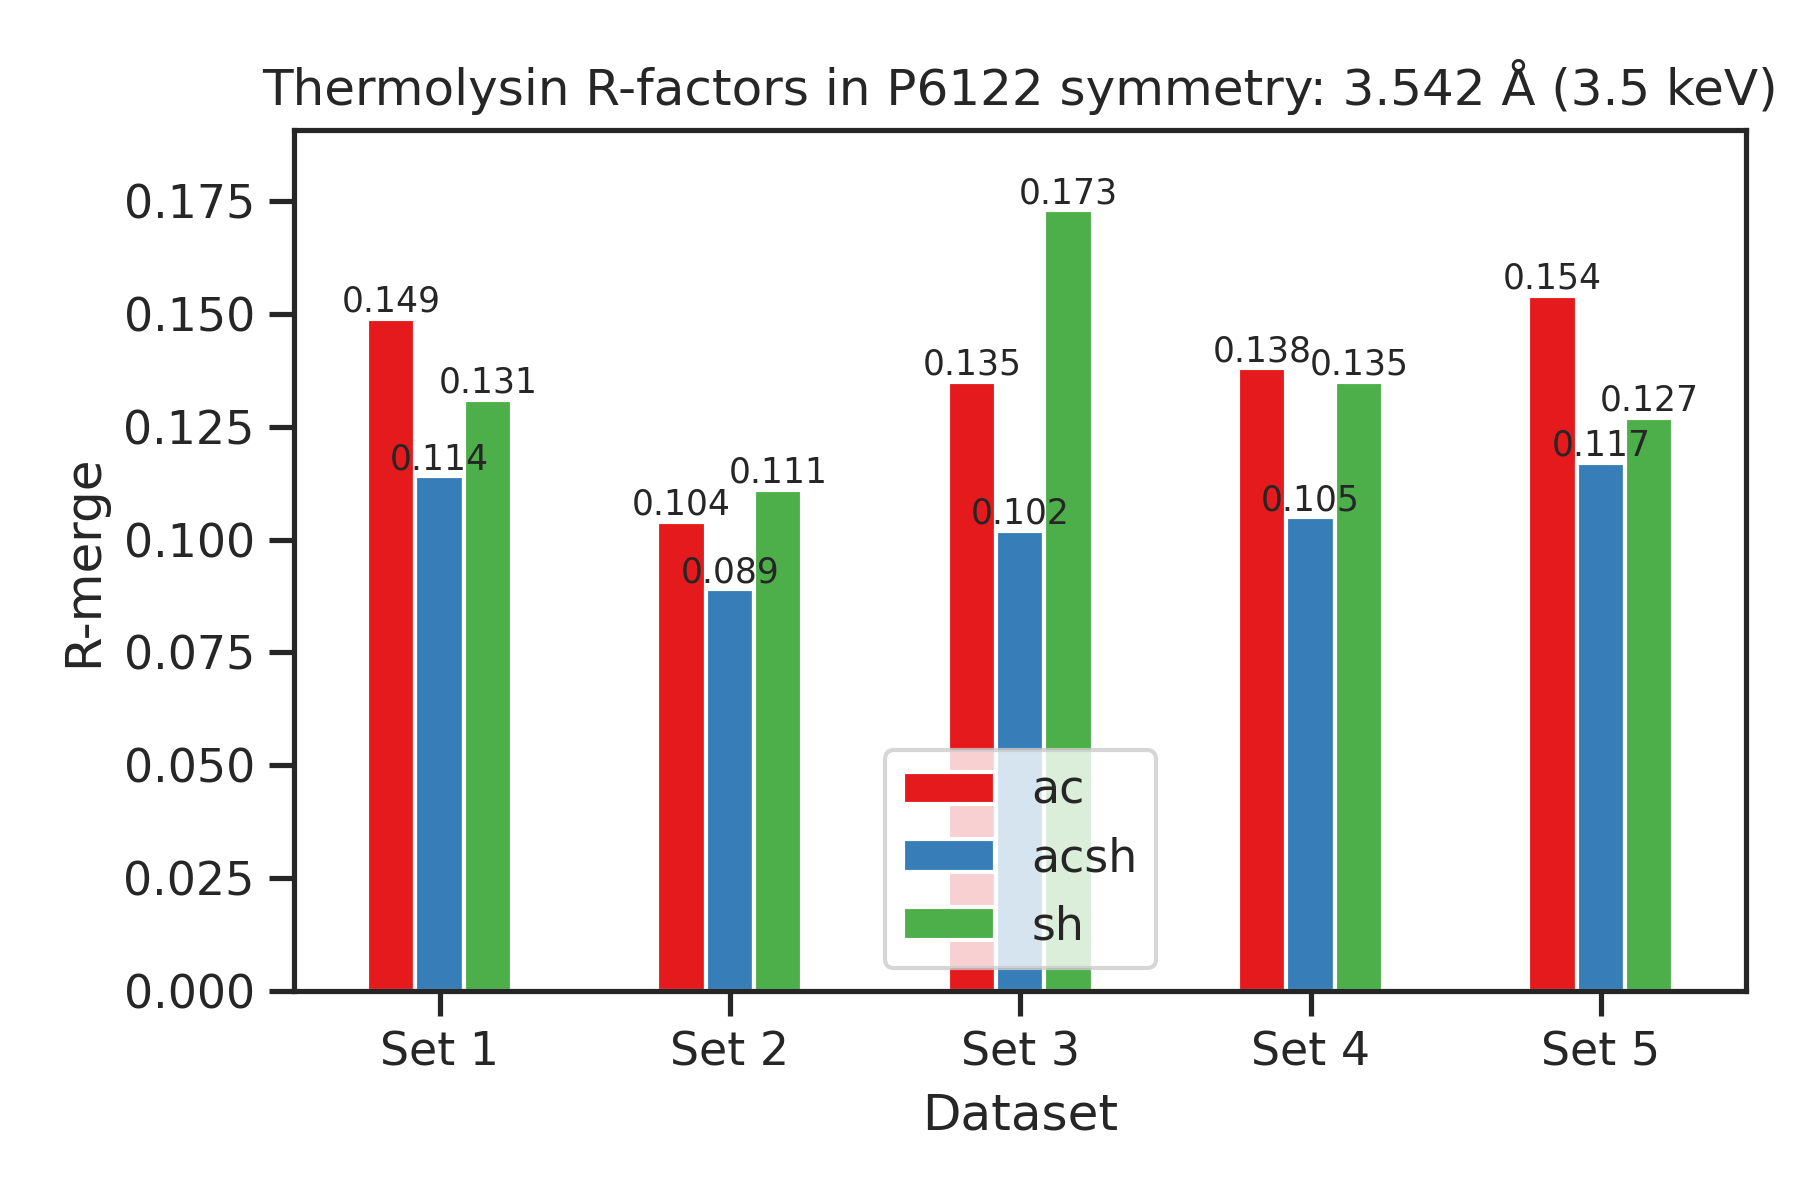
\includegraphics[width = 0.5\textwidth]{plots/exp1/tlys_2_P6122/3p5_rmerges.png}
    \end{tabular}
    \caption{Merging statistics for Thermolysin 2 at 3.5 keV.}
    \label{fig:tlys_2_3p5}
\end{figure}

Following collection of reflection data, the AnACor results are used for structure refinement in Dimple to generate anomalous density peaks for all the detected anomalous atoms and molecules, based on the provided model. In thermolysin, the relevant anomalous groups are two conformations of methionine (205 and 120), and a zinc atom. The results of Thermolysin 2 are shown in \cref{fig:tlys2_met_peaks_3p0} and \cref{fig:tlys2_met_peaks_3p5}.

Datasets across the same energy processed in P\textsubscript{1} were additionally merged to increase the multiplicity of the low symmetry space group, and the results of processing Thermolysin 1 and Thermolysin 2 in P\textsubscript{1} repeat the same trend seen for \textit{P}6\textsubscript{1}22.

\begin{figure}[h]
    \centering
    \begin{tabular}{cc}
    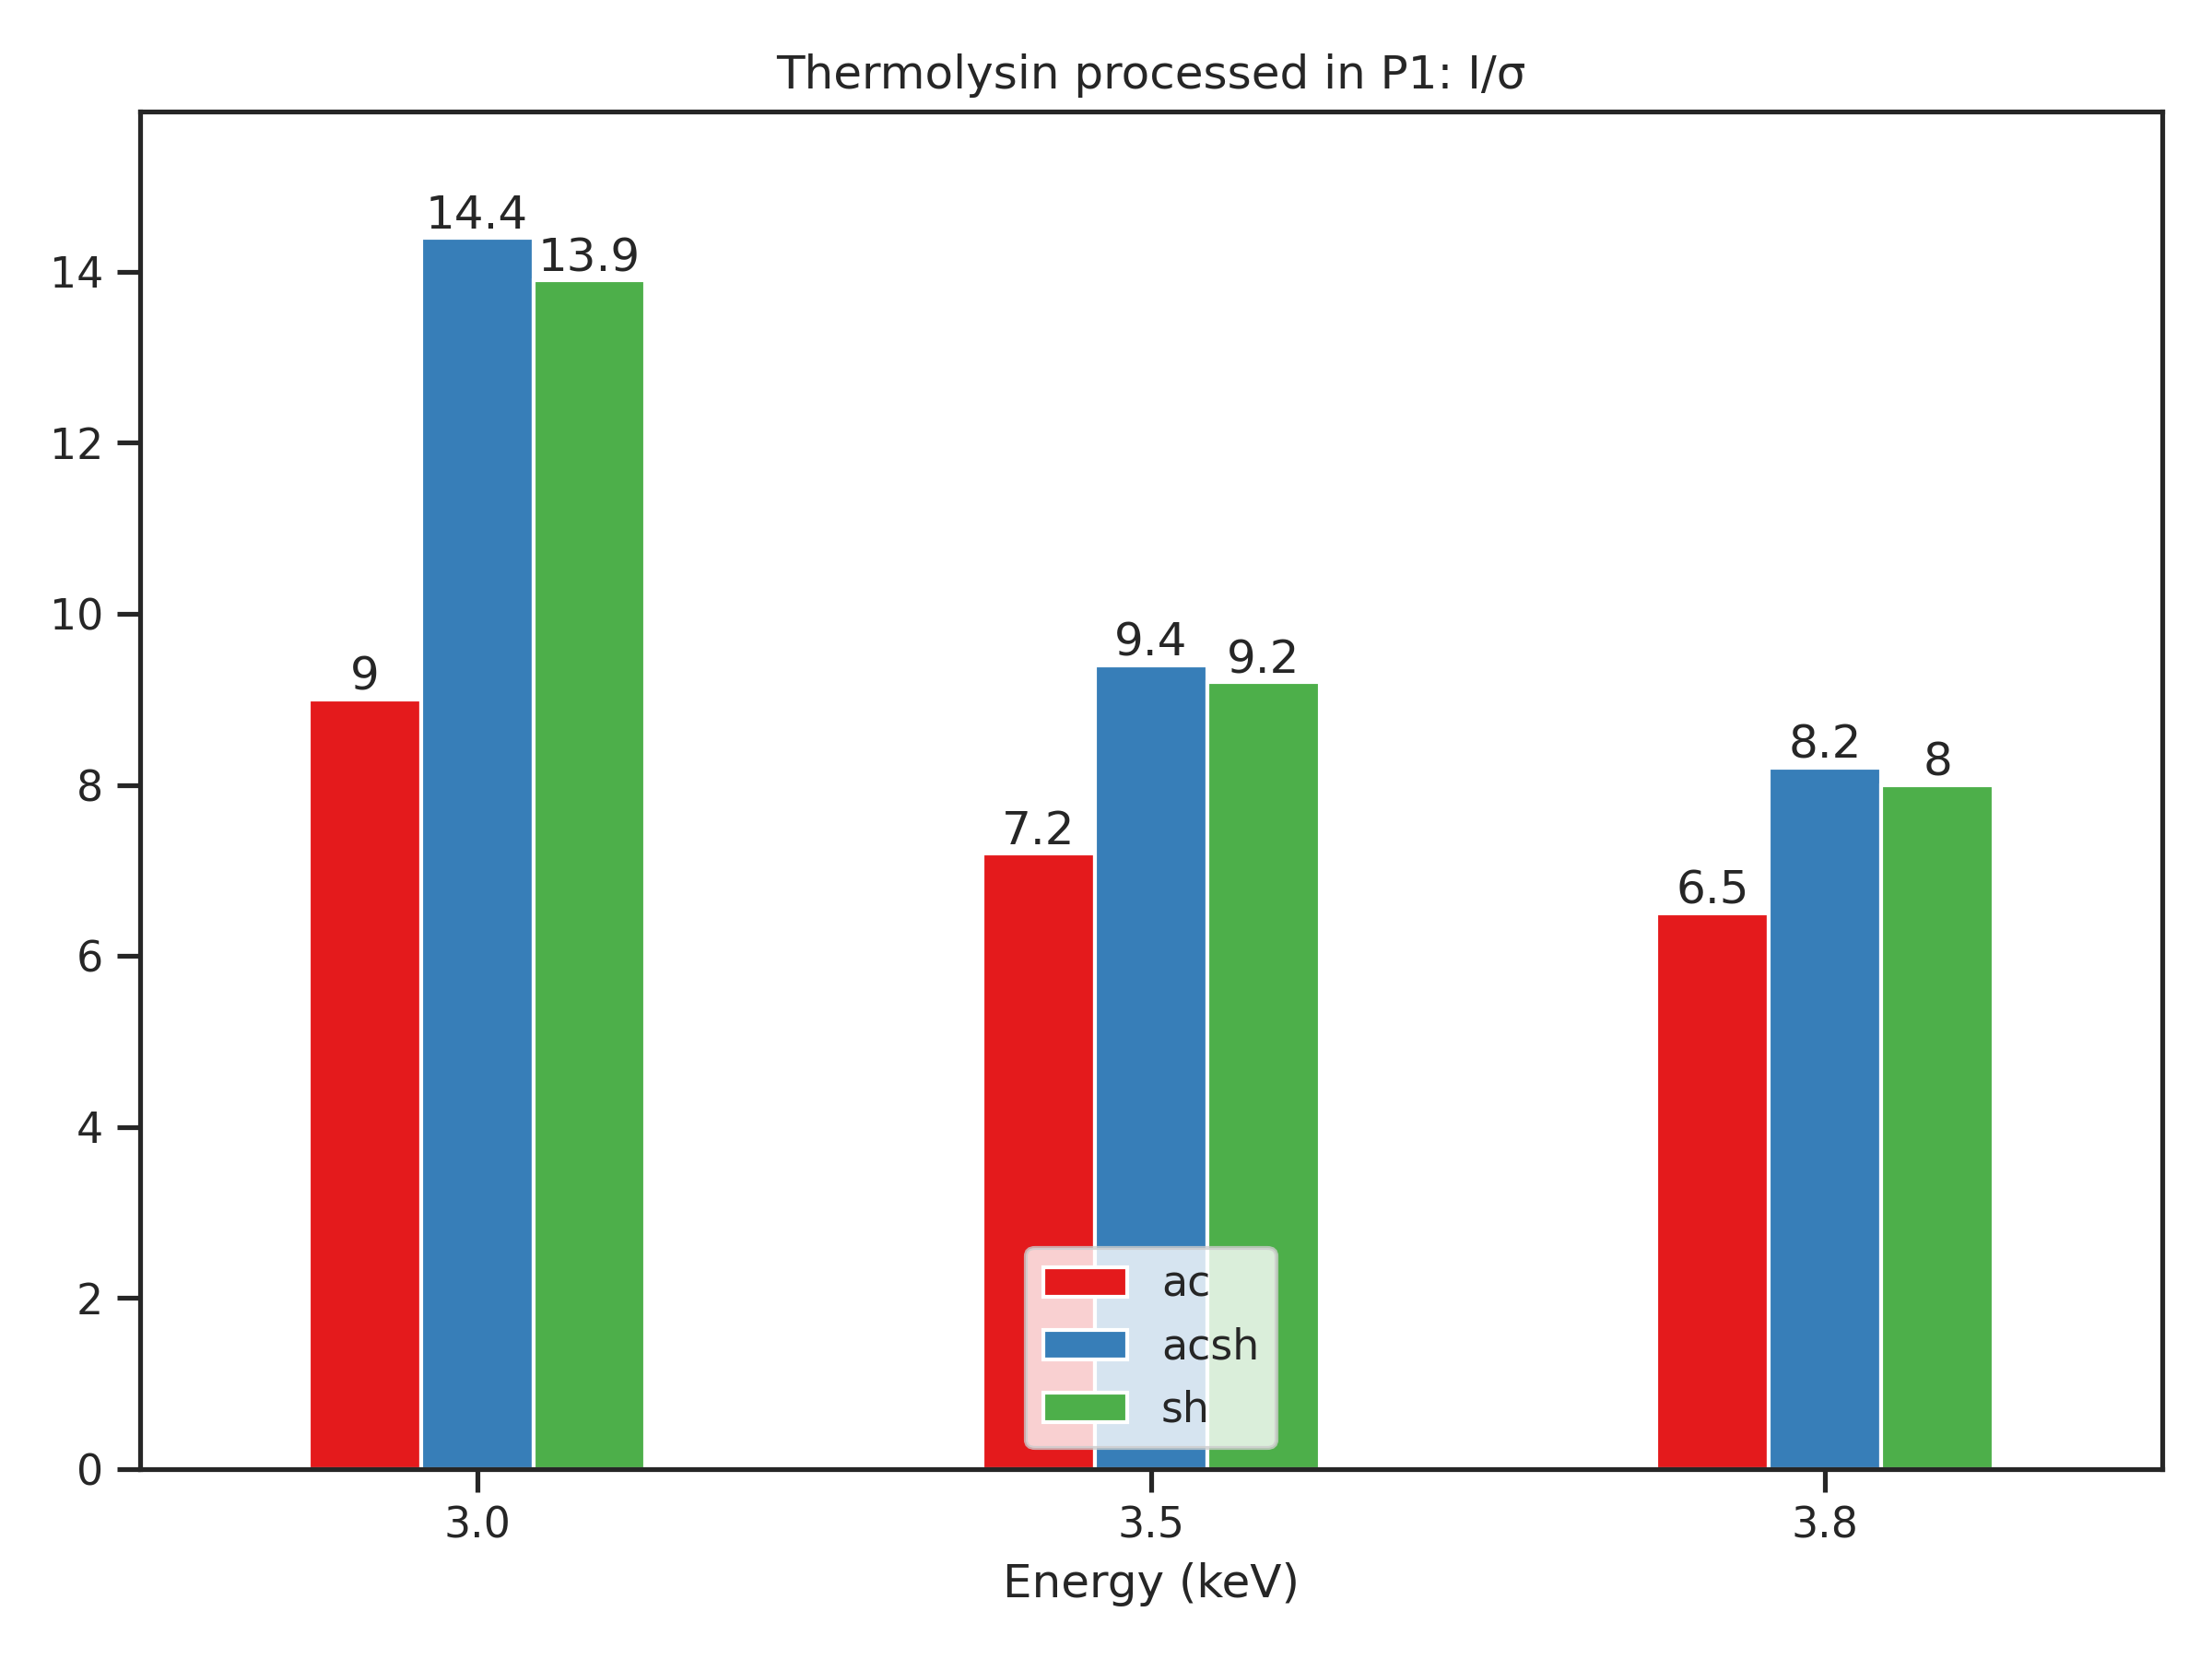
\includegraphics[width = 0.5\textwidth]{plots/exp1/tlys_9_P1/I_over_sigma.png} & 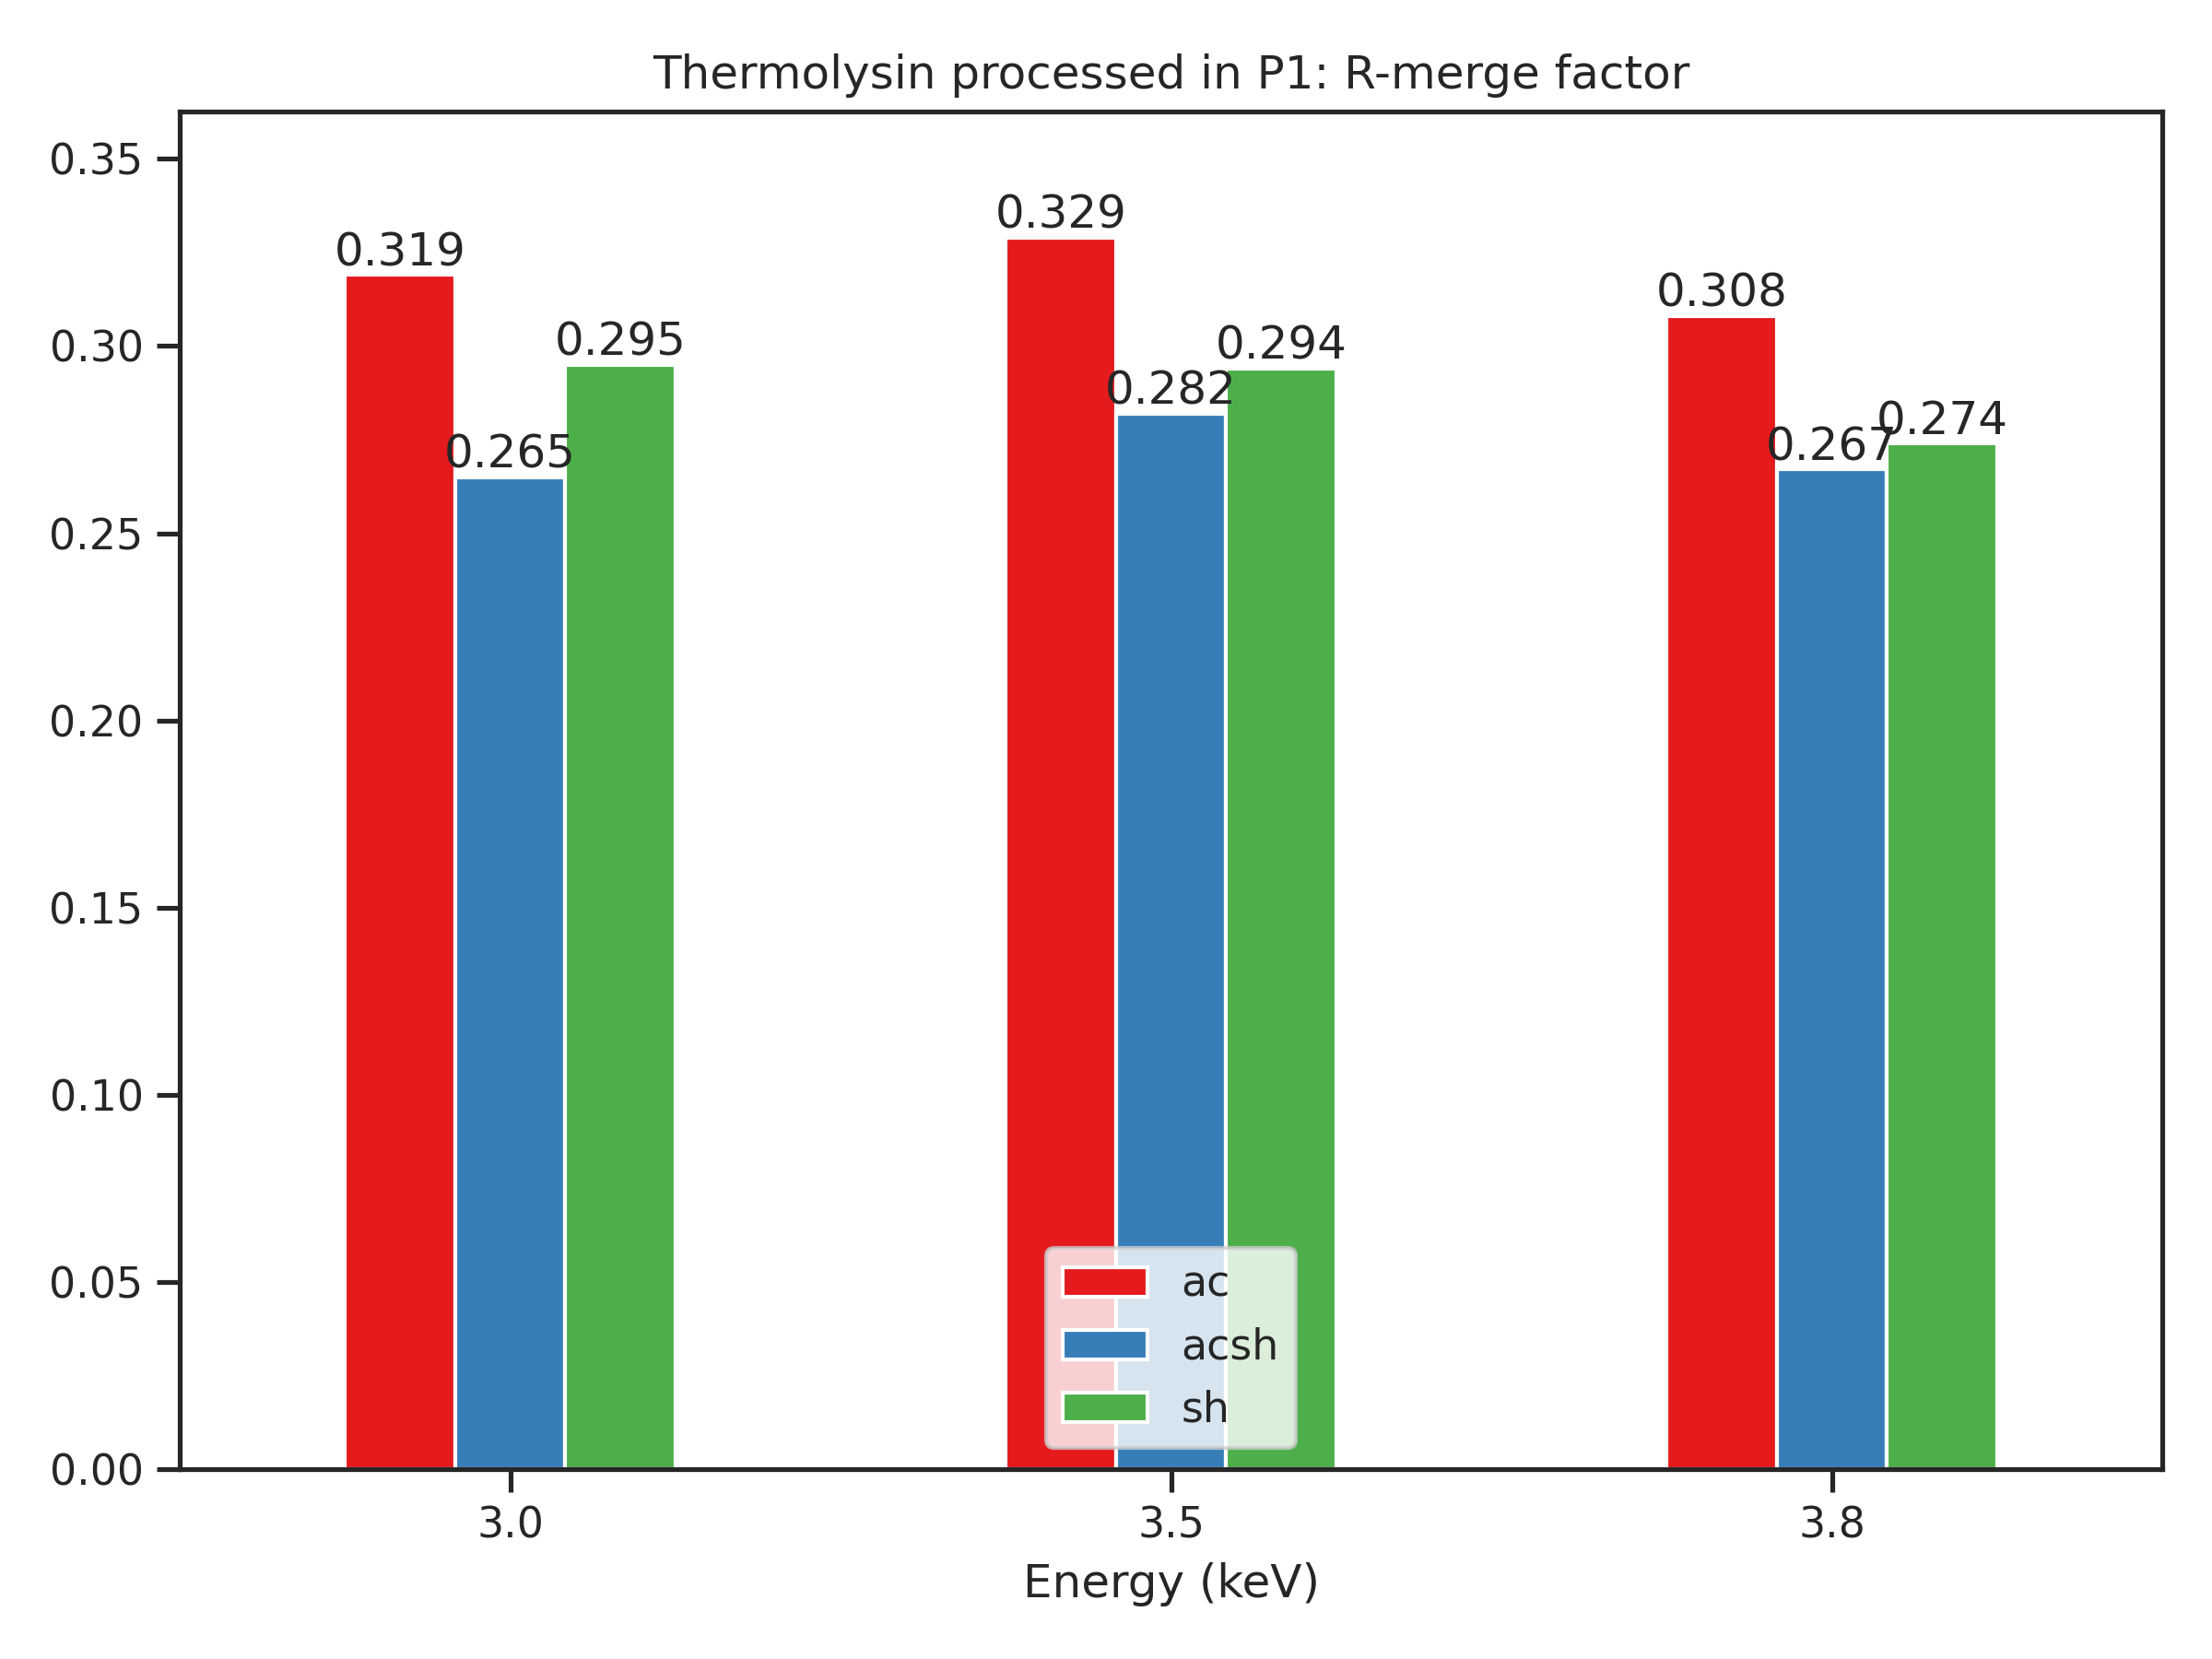
\includegraphics[width = 0.5\textwidth]{plots/exp1/tlys_9_P1/rmerges.png}
    \end{tabular}
    \caption{Caption}
    \label{fig:tlys_2_p6}
\end{figure}

\begin{figure}[h]
    \centering
    \begin{tabular}{cc}
    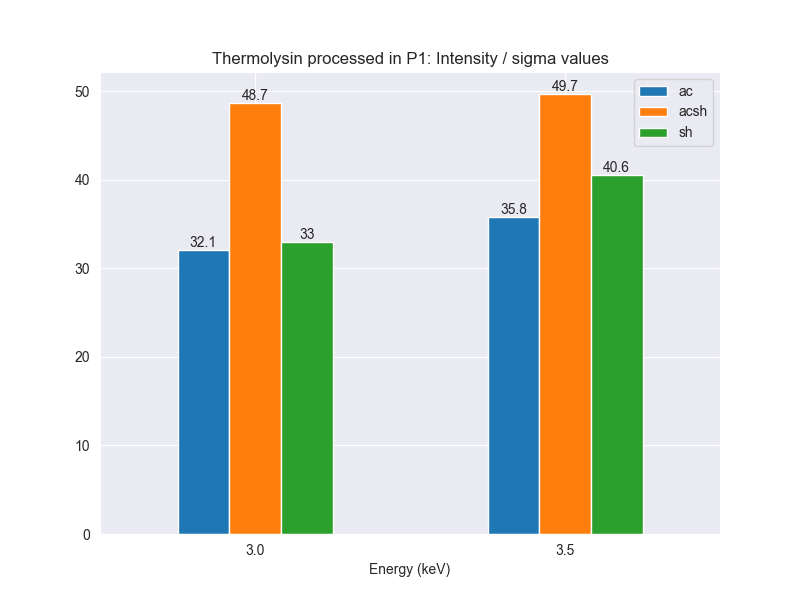
\includegraphics[width = 0.5\textwidth]{plots/exp1/tlys_2_P1/I_over_sigma.png} & 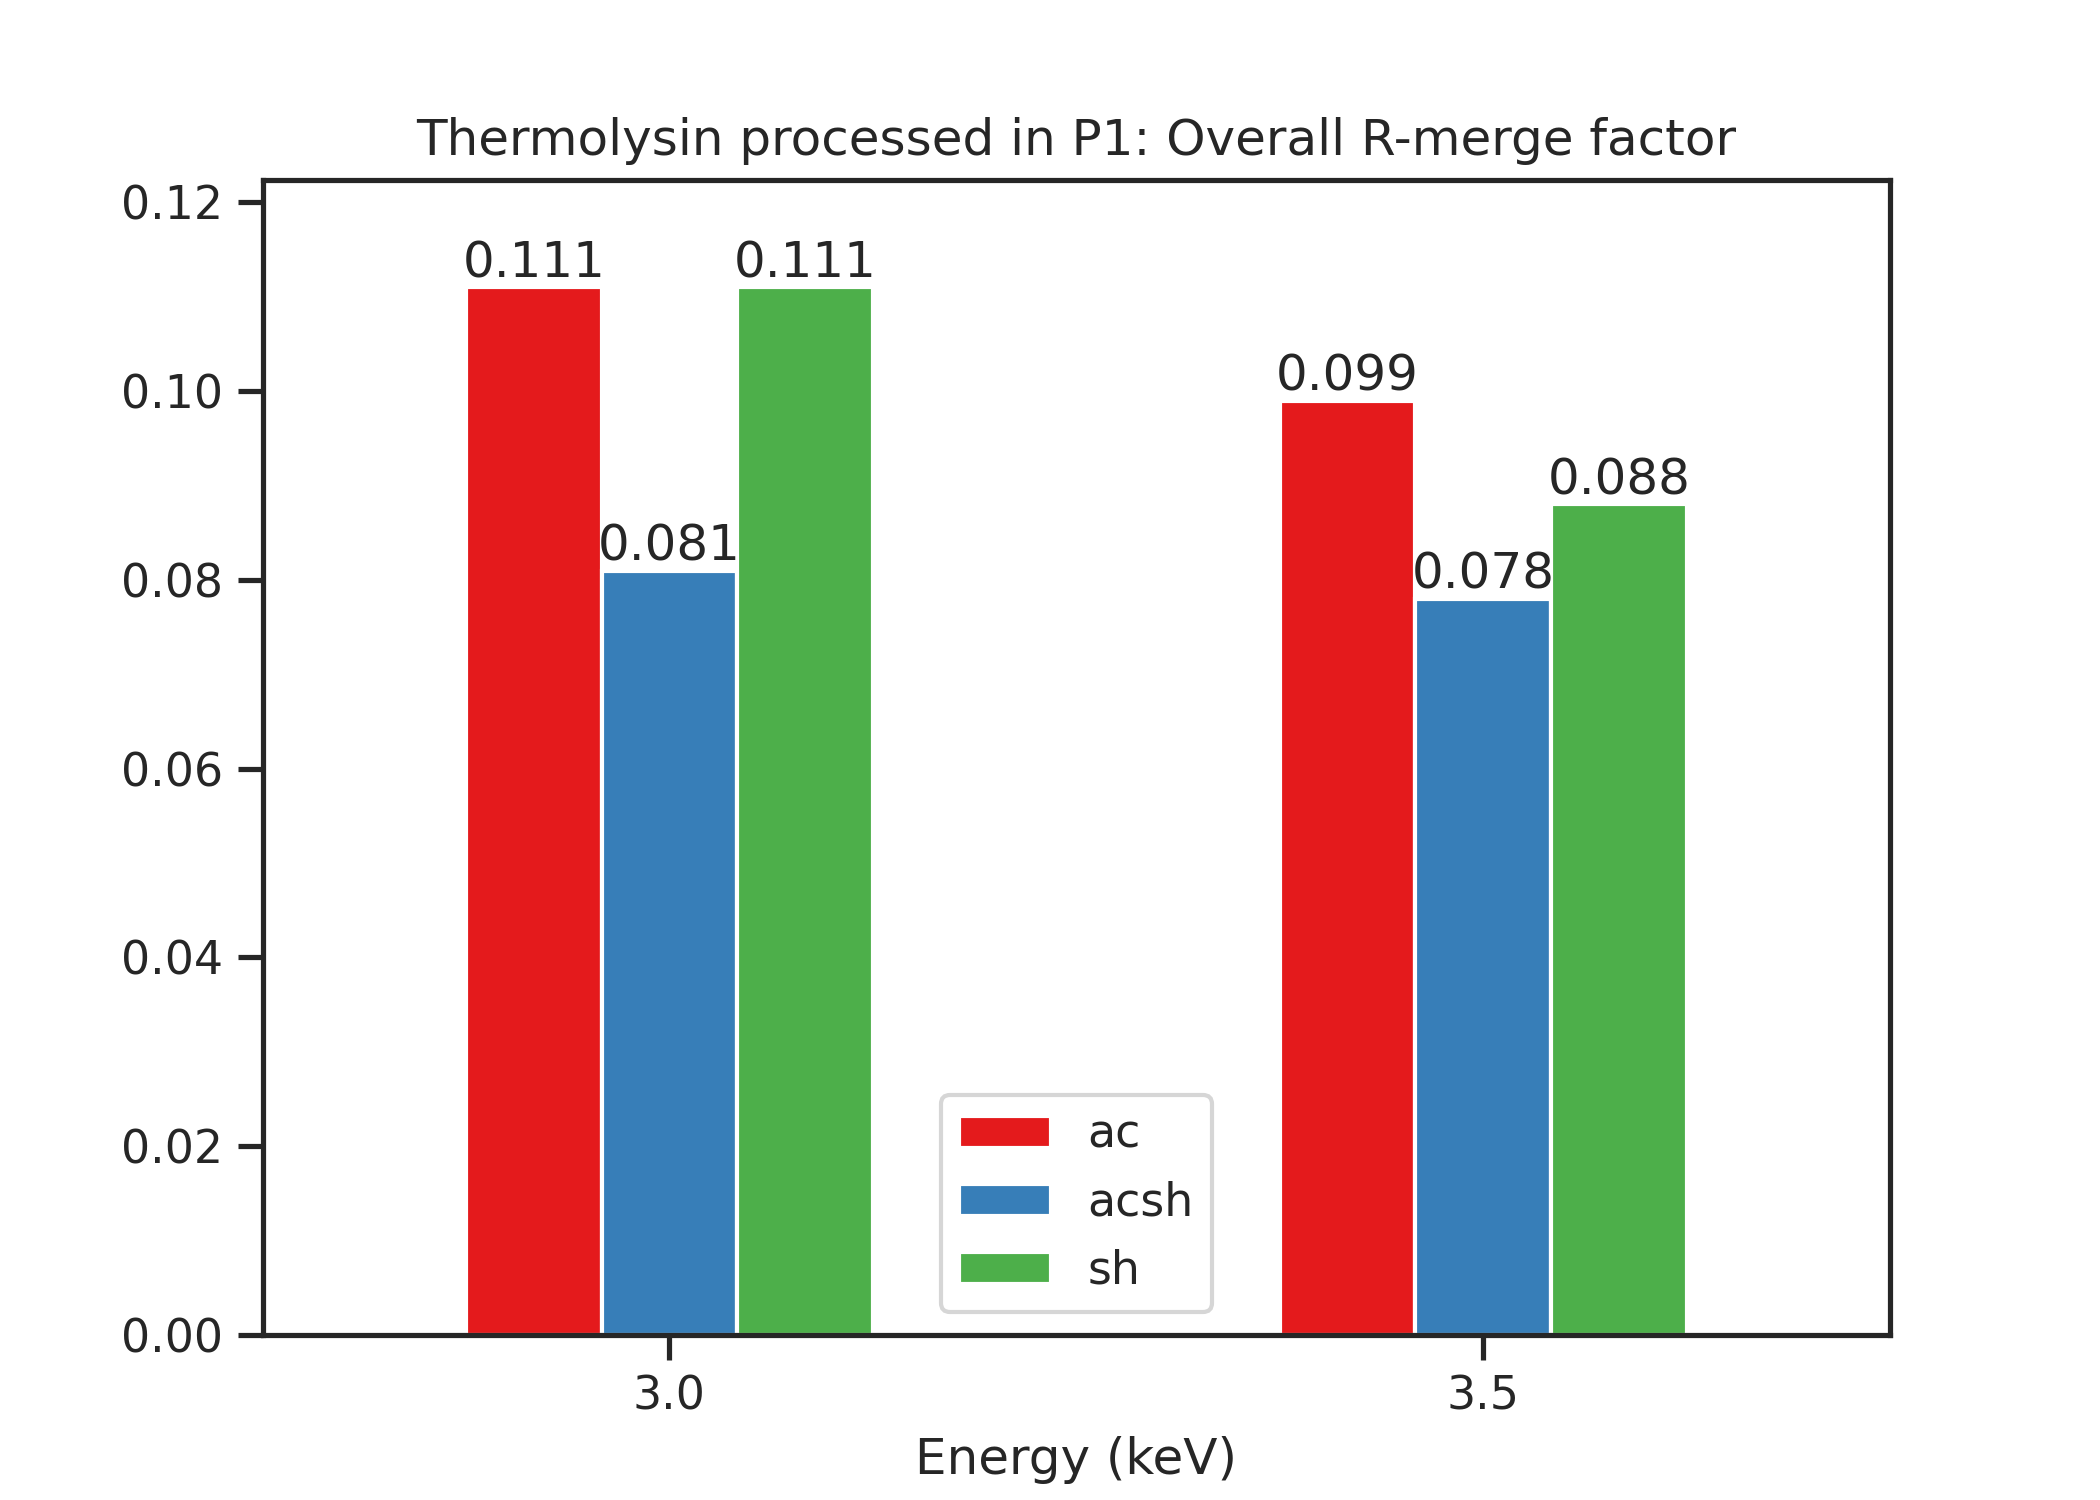
\includegraphics[width = 0.5\textwidth]{plots/exp1/tlys_2_P1/rmerges.png}
    \end{tabular}
    \caption{Caption}
    \label{fig:tlys_2_p6}
\end{figure}

\subsection{Analytically-corrected Tomography data in $f"$-refinement for ion identification}

%As of this year, I23 has established a new method of ion identification using anomalous scattering known as f" refinement. This protocol uses a programme known as Phenix which has a feature for estimating the f' and f" values of a given element based on the (mtz and pdb) of the collected crystal data. The f"-refinement is becoming a routinely-used feature of ion identification due to the long wavelength capabilities of the beamline. 

The reflection data from Thermolysin 2 that was produced across all three correction methods in the prior experiment were then used in the Phenix in the platform known as \textit{phenix.refine}. This platform allows for the refinement of absorption parameters $f'$ and $f"$ based on the reflection data and \textit{pdb} structure provided. As described in the methodology, the first stage of \textit{phenix.refine} uses the reflection data provided to produce a modified version of the molecular structure in \textit{pdb} format. This updated molecular structure is then used in the second stage with the same reflection data to estimate the theoretical $f'$ and $f"$ values of specified atoms that are believed to be in the structure. In the case of this experiment, $f'$ was fixed to its theoretical value for a given atom and energy, allowing for an experimental $f"$ to be refined. This value is then corroborated with the theoretical value to determine whether the atom type can be correctly identified.% test the ability of identifying atoms of sulphur and zinc in the crystal by determining their $f"$ peak.


\begin{figure}[h]
    \centering
    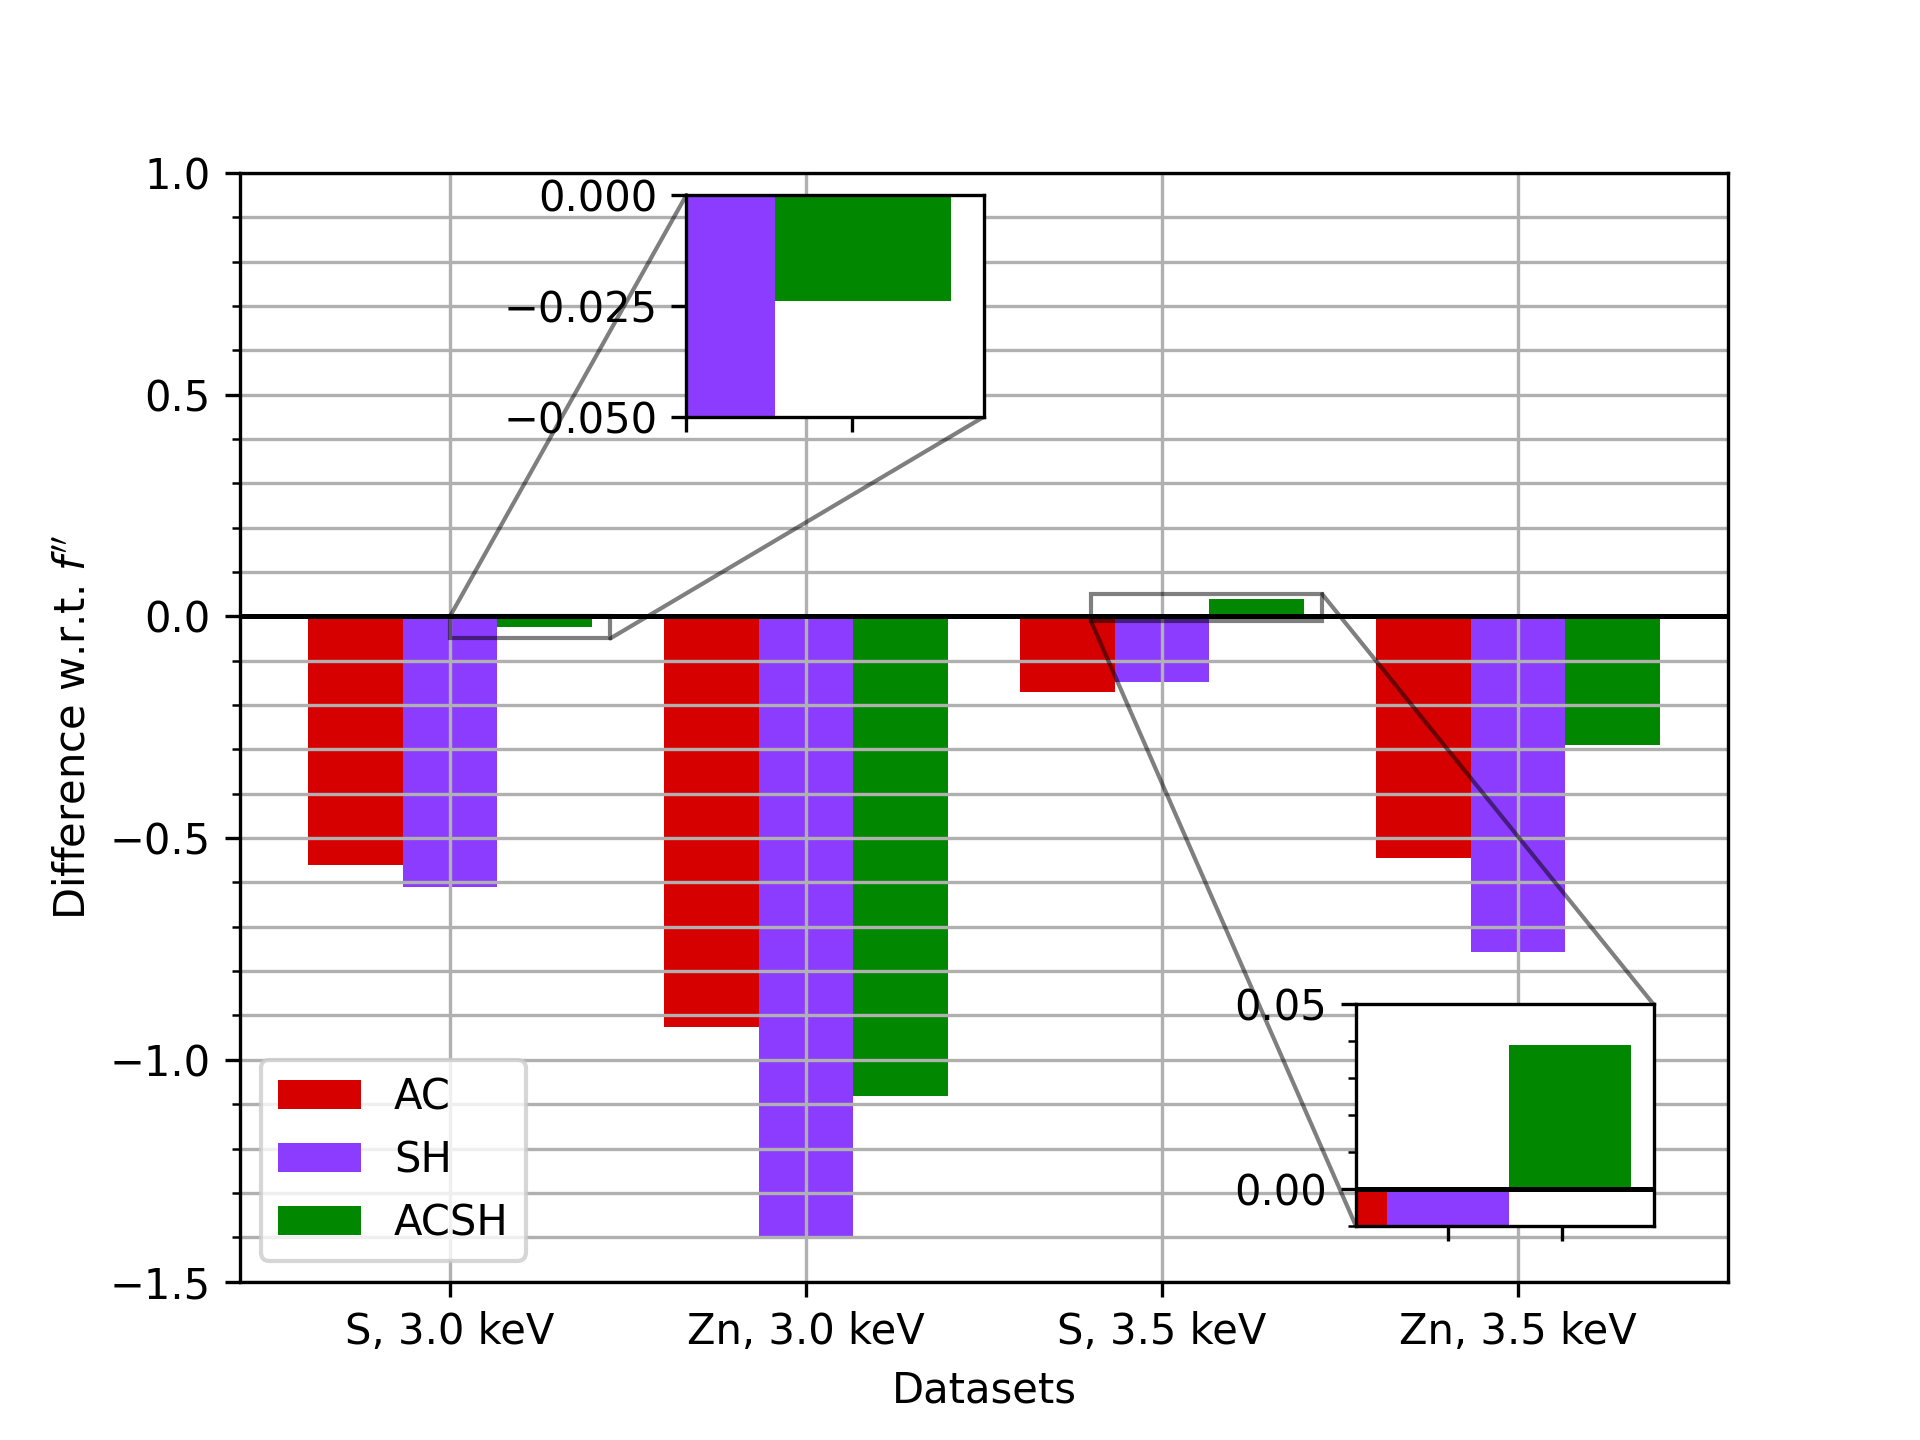
\includegraphics[width = 0.7\textwidth]{plots/phenix_plot_Pat.png}
    \caption{Difference with respect to theoretical $f"$ for atoms of sulphur and zinc in Thermolysin 2. Values obtained from Phenix.refine in the Phenix software package for Macromolecular structure determination.}
    \label{fig:phenix_plot}
\end{figure}

Results from Phenix refine for the six sets of reflection data of Thermolysin 2 (three methods across 3.0 and 3.5 keV) are shown in \cref{phenix_table} and visualized in \cref{fig:phenix_plot}. It is clear that refinement of the sulphur edge was much more precise than for zinc.


\subsection{Tomography-based corrections with laser-shaped samples}

\begin{figure}[h]
    \centering
    \begin{tabular}{cc}
    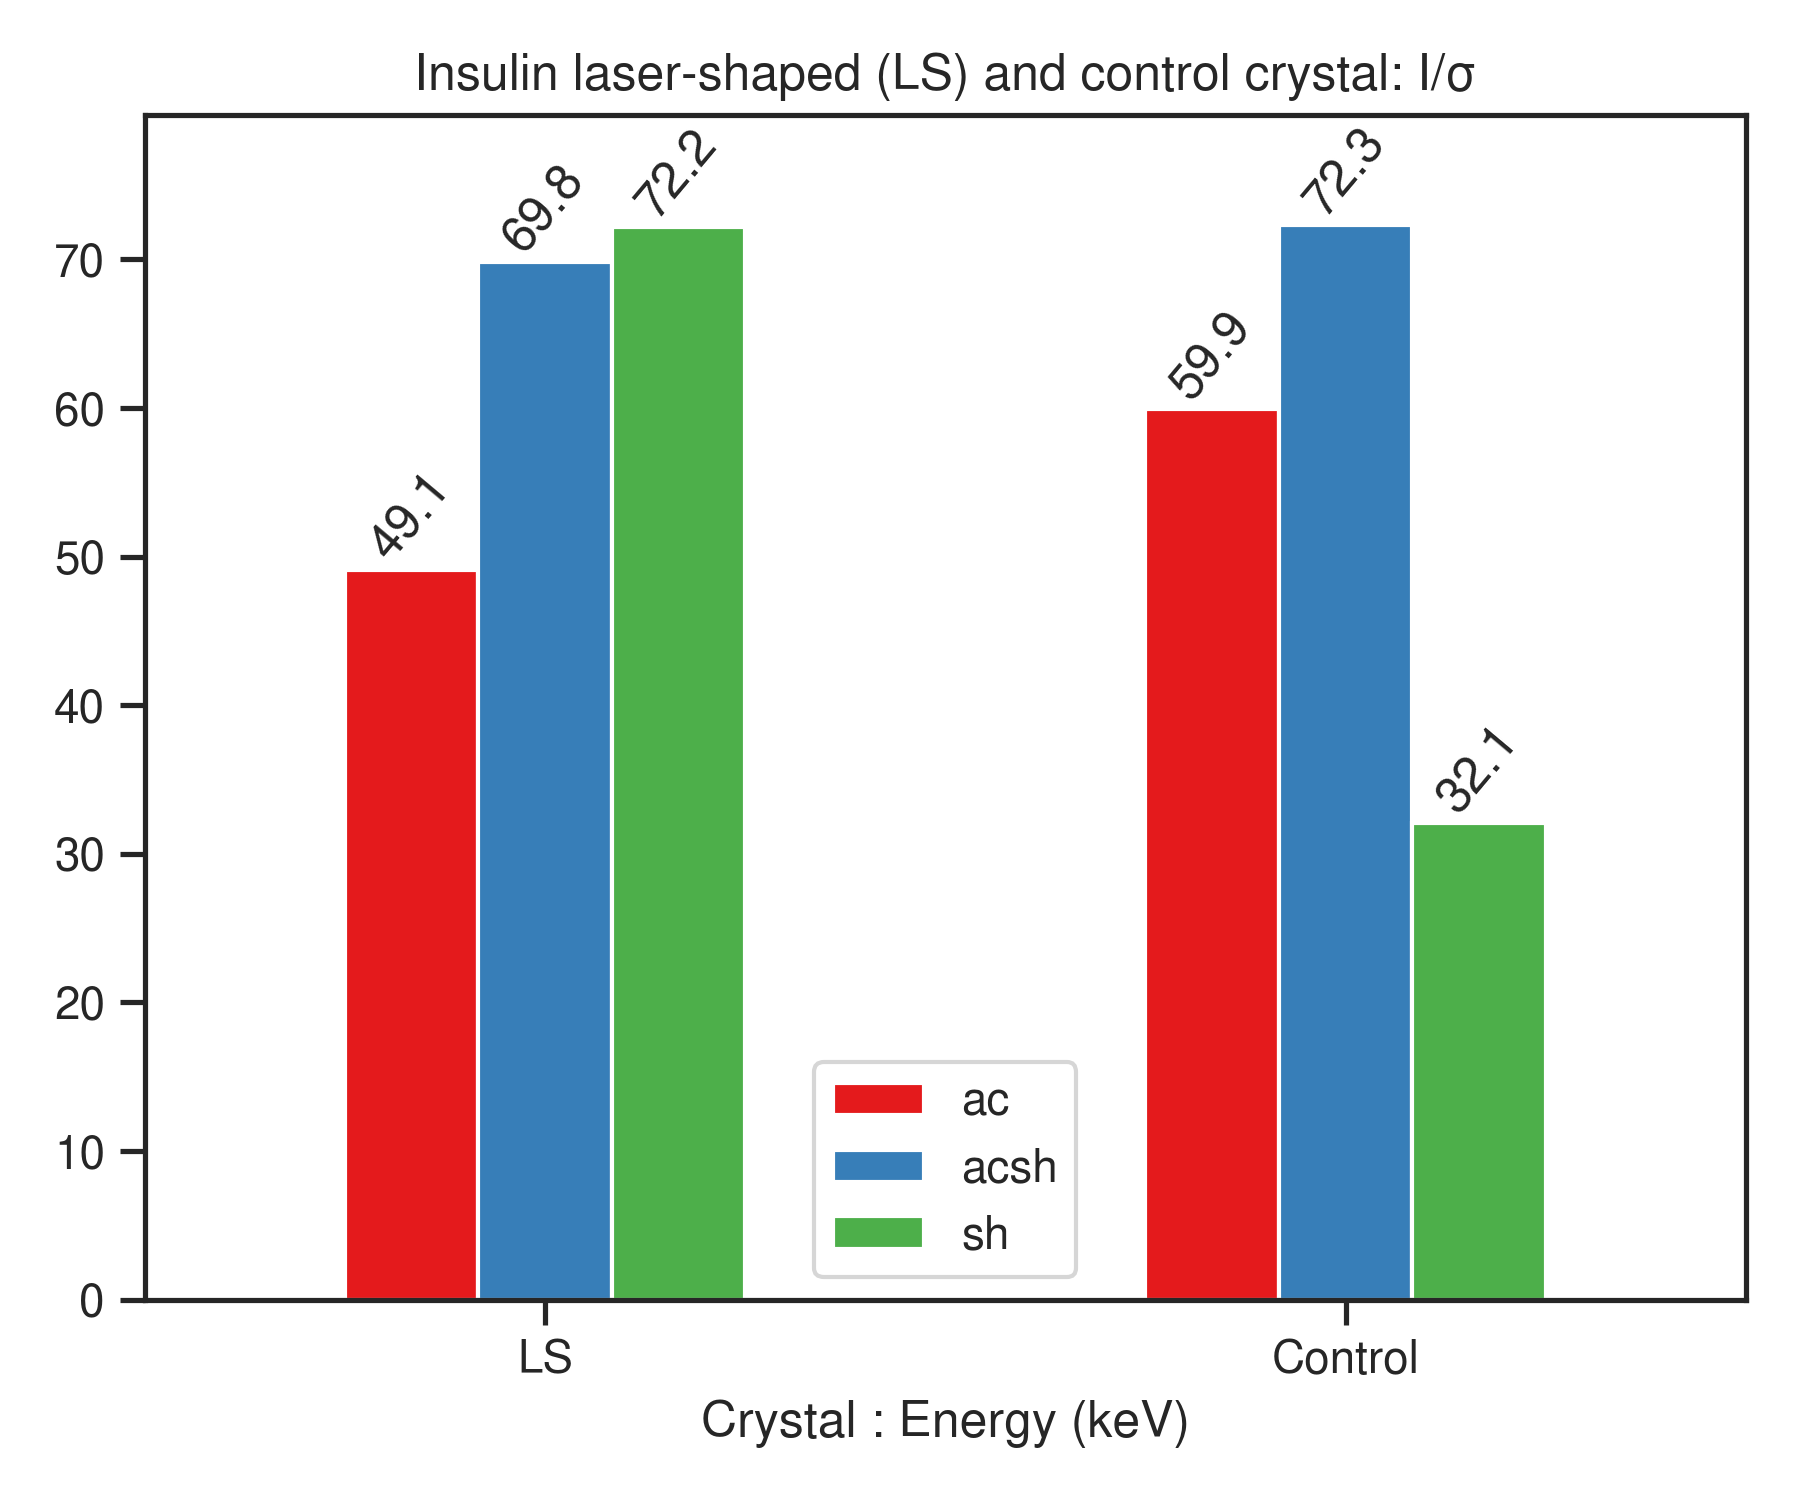
\includegraphics[width = 0.5\textwidth]{plots/exp2/ins_I_over_sigma.png} & 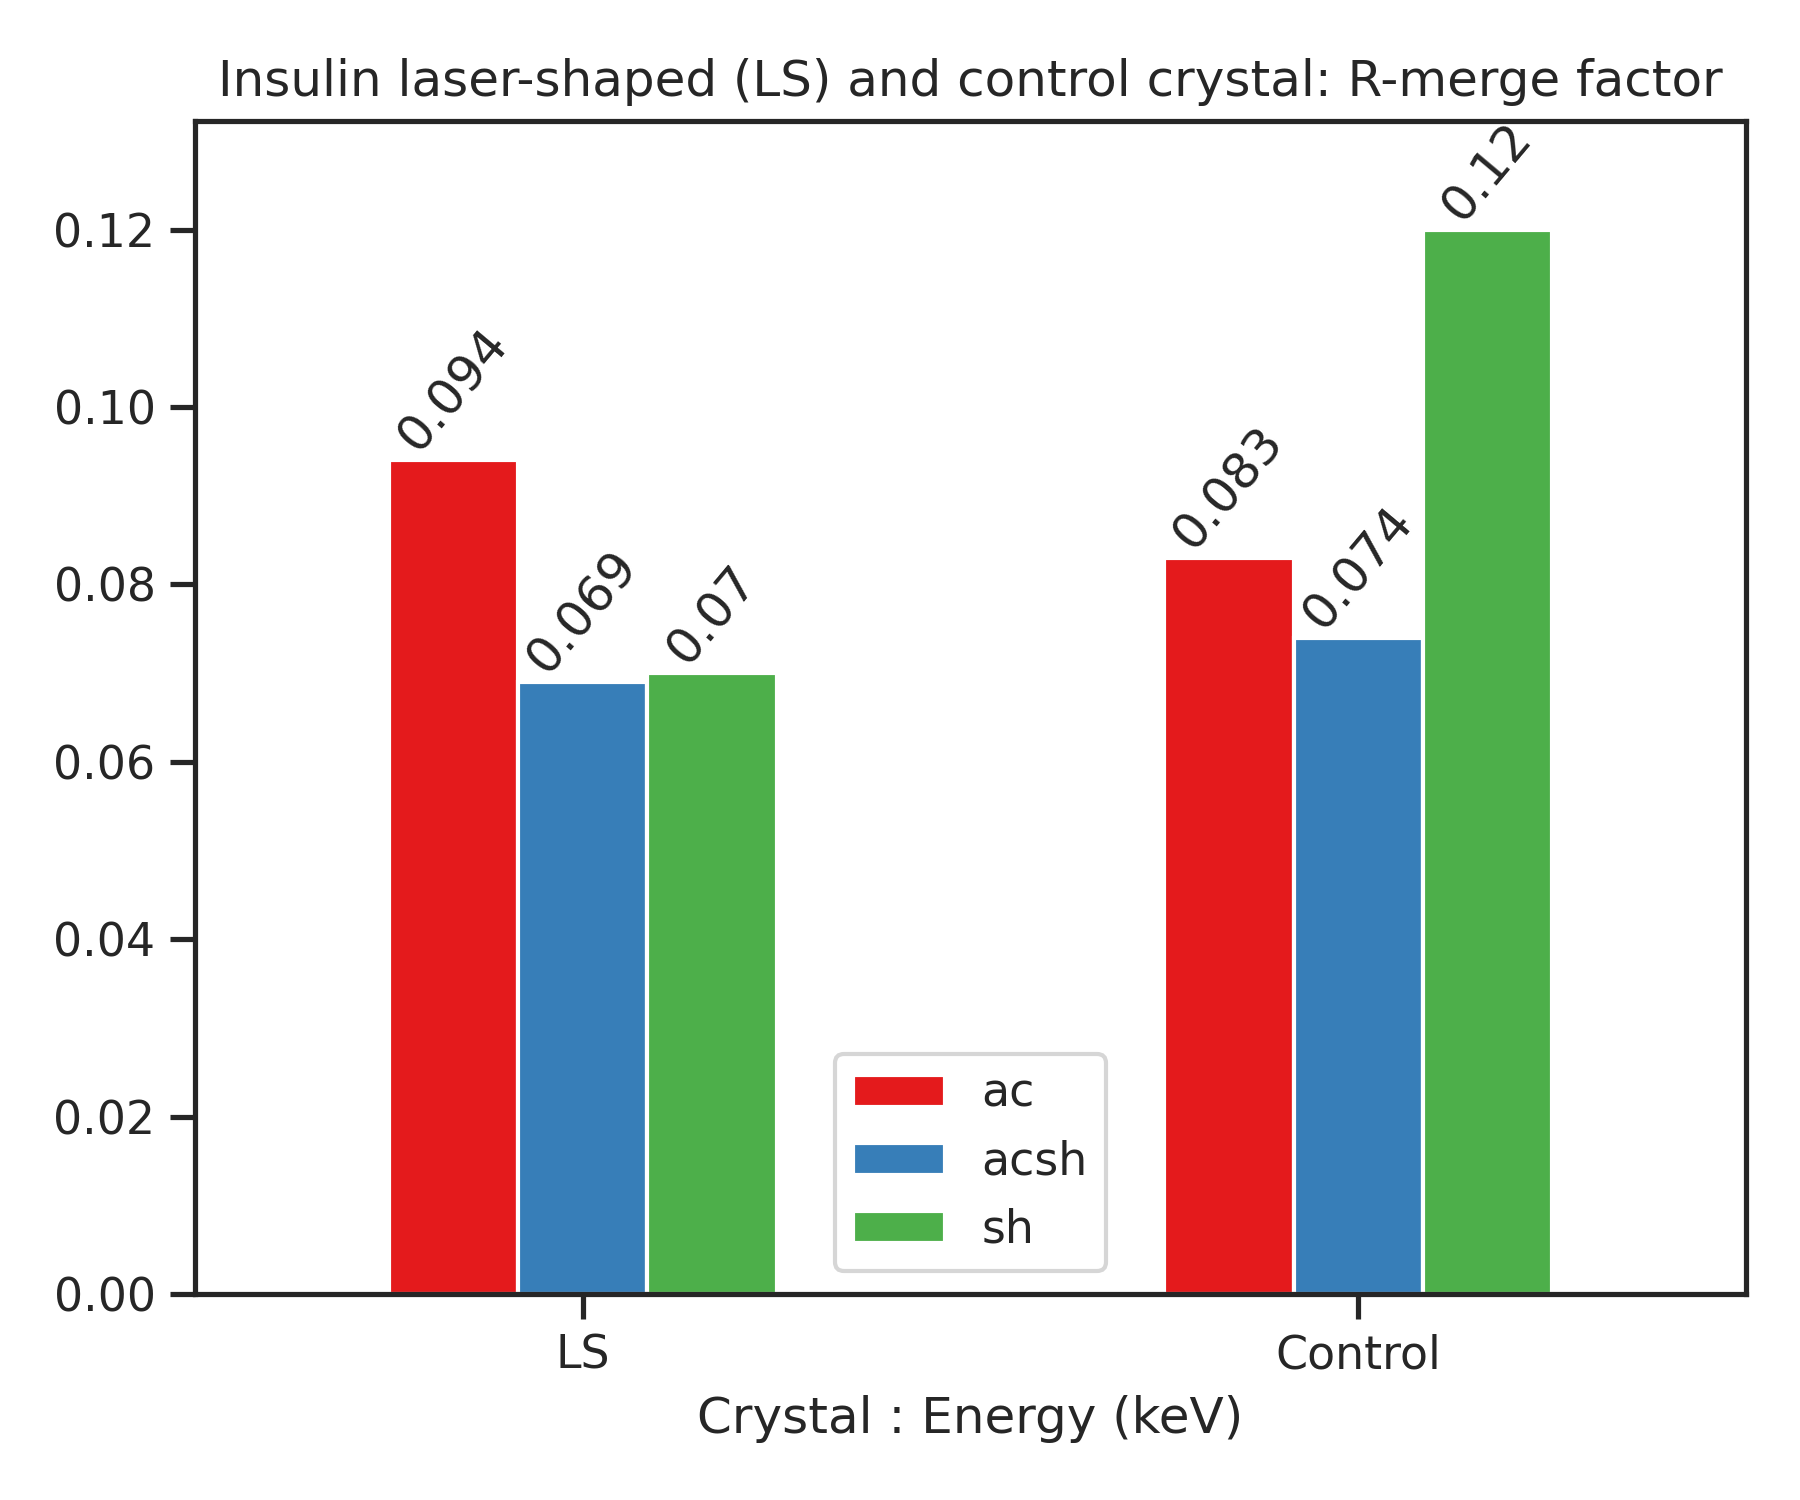
\includegraphics[width = 0.5\textwidth]{plots/exp2/ins_rmerges.png}
    \end{tabular}
    \caption{Merging statistics for the laser-shaped and control crystals of insulin at 3.0 keV.}
    \label{fig:insulin}
\end{figure}

\begin{figure}[h]
    \centering
    \begin{tabular}{cc}
    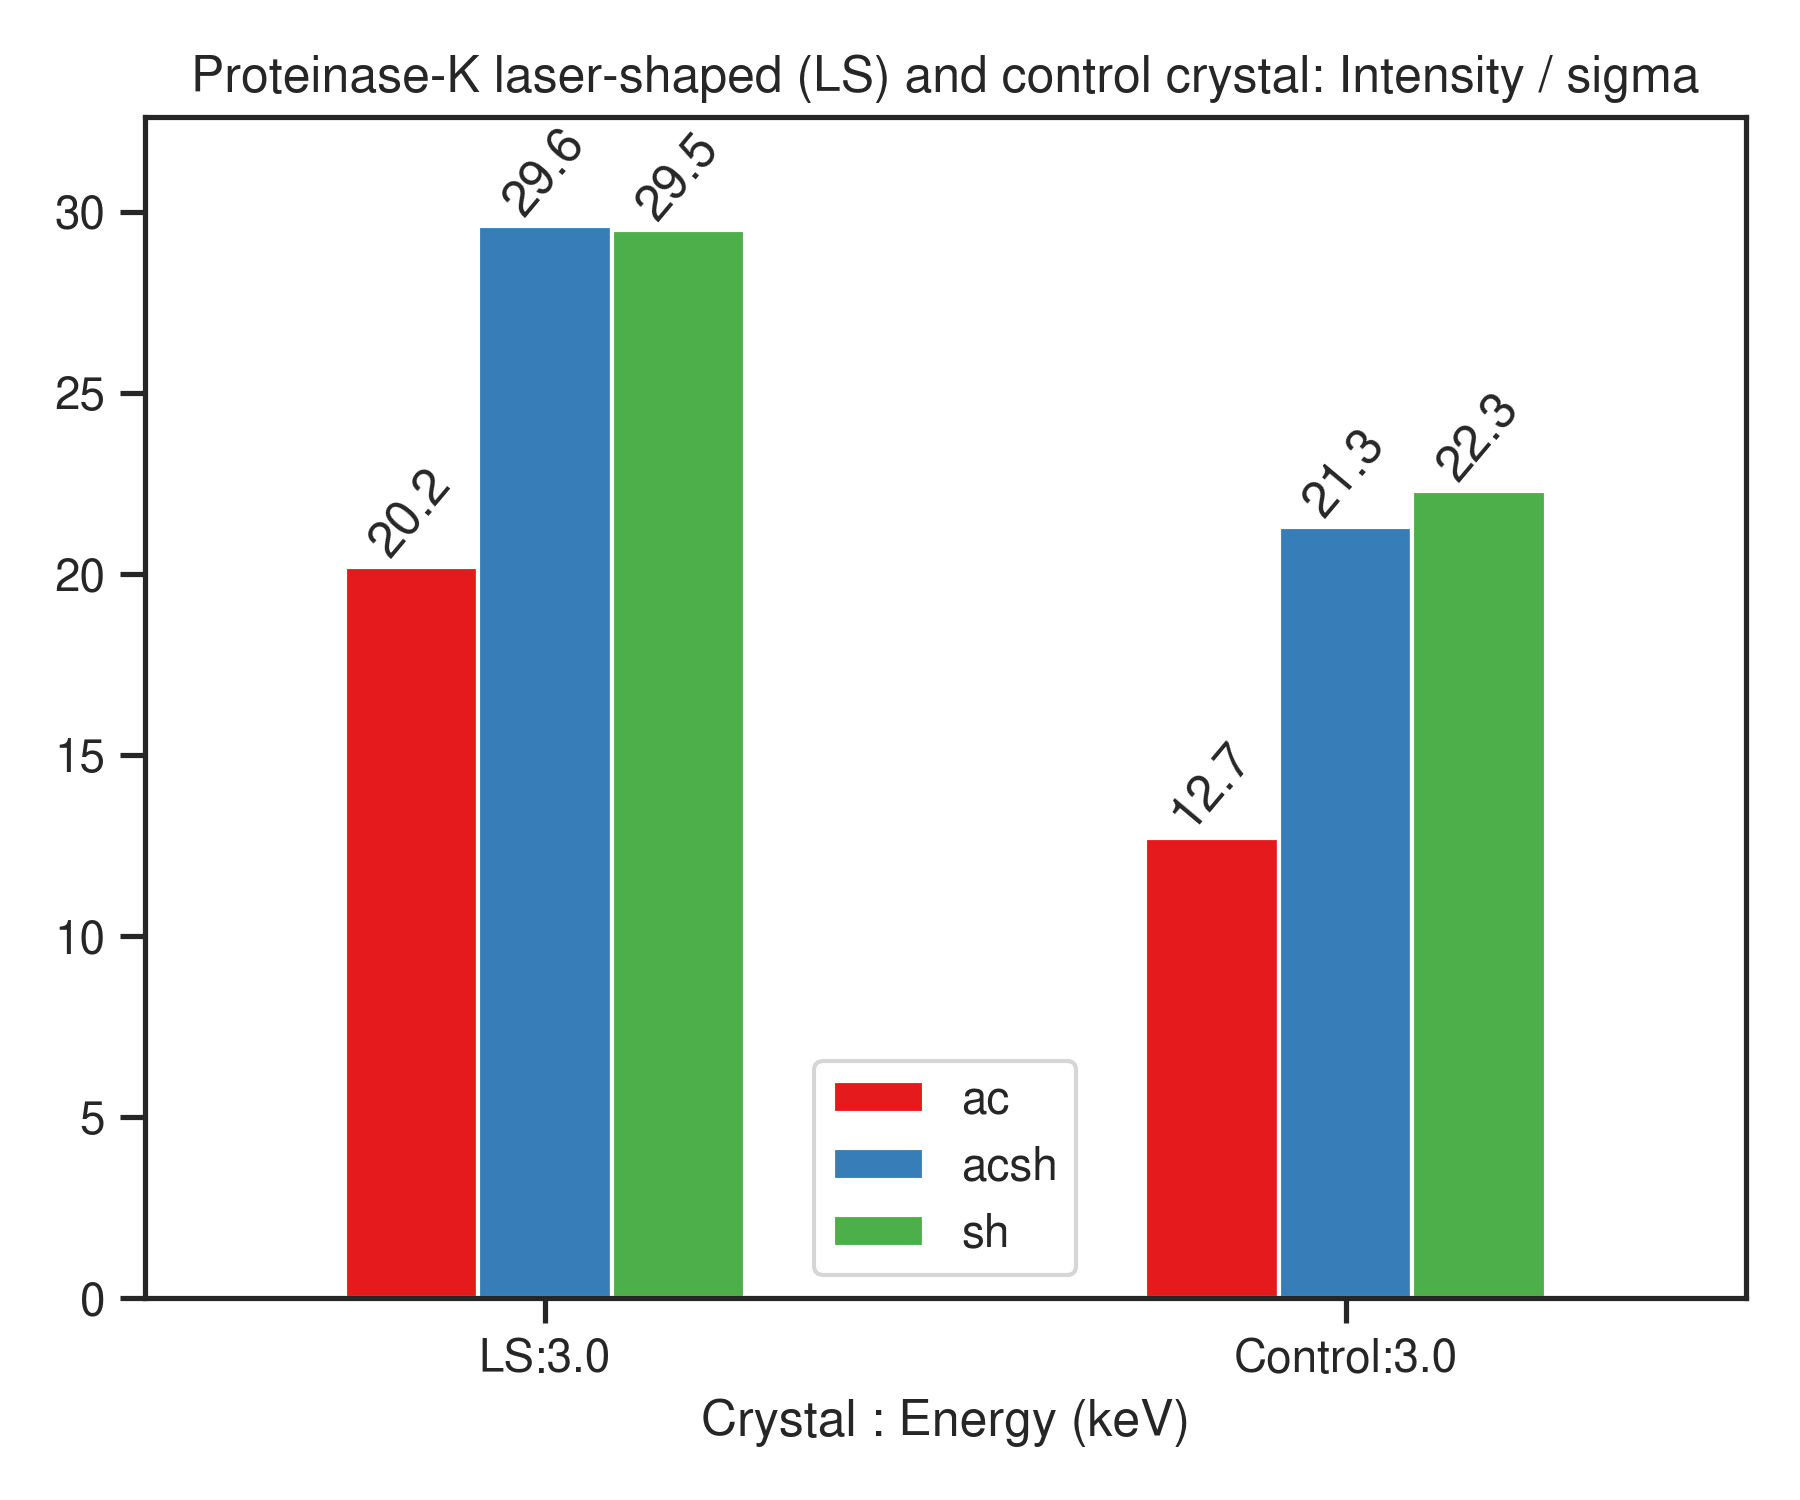
\includegraphics[width = 0.5\textwidth]{plots/exp2/prot_I_over_sigma.png} & 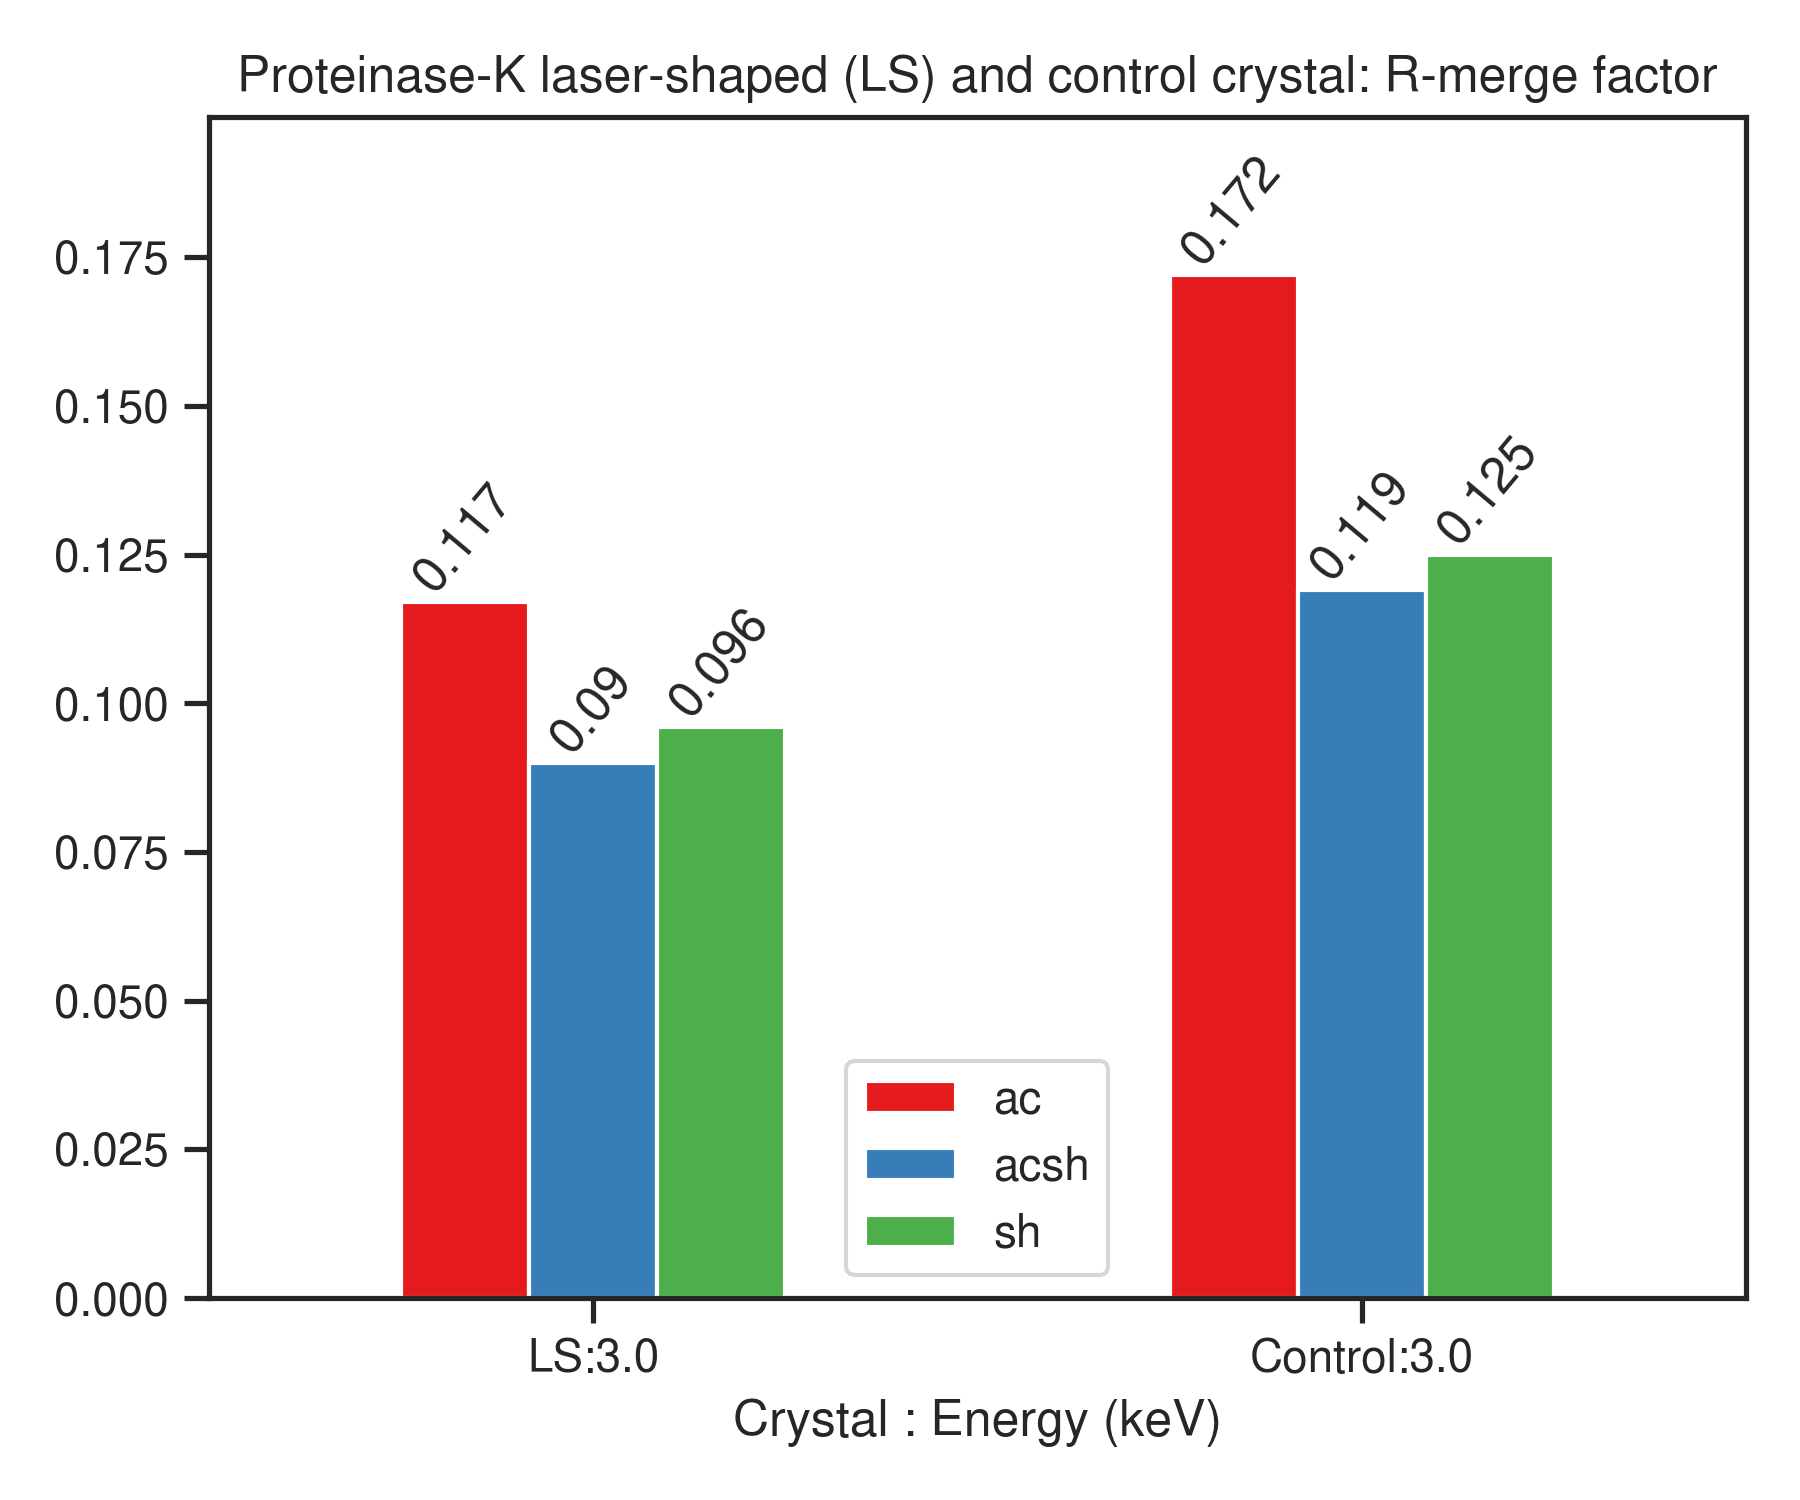
\includegraphics[width = 0.5\textwidth]{plots/exp2/prot_rmerges.png}
    \end{tabular}
    \caption{Merging statistics for the laser-shaped and control crystals of proteinasek at 3.0 keV.}
    \label{fig:proteinasek}
\end{figure}


Testing tomo on lysosyme to try to detect sodium anomalous signal

Mention LASER-shaping already worked on identifying magnesium in topoisomerase crystals. Hypothesis: tomography can do the same



\subsection{Errors and Improvement}

Faults in anacor thresholding, particularly at processing datasets collected at multiple energies

segmentation at high contrast

There are several challenges associated with the segmentation of X-ray data of protein crystals.

\section{Conclusion and Future Outlooks}

Future experiment on determining the presence of magnesium in topoisomerase



%Appendix and Backmatter
\printbibliography
\newpage

\appendix
\noindent
%\twocolumn
\section{Appendix}
\subsection{A: Segmentation Models}

\begin{figure}[h]
    \begin{tabular}{cc}
    	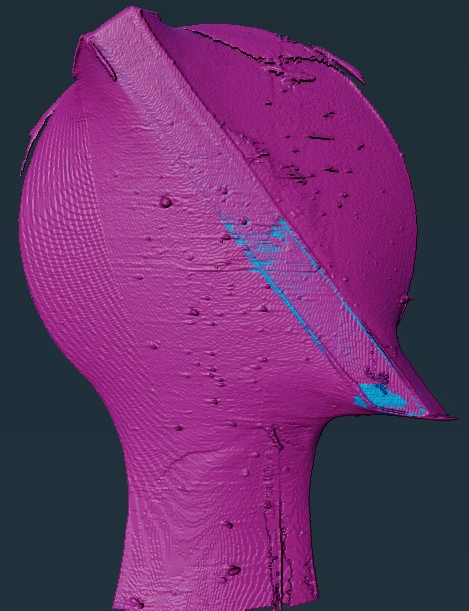
\includegraphics[height=7cm ]{images/avizo_flats/tlys9.jpg} & 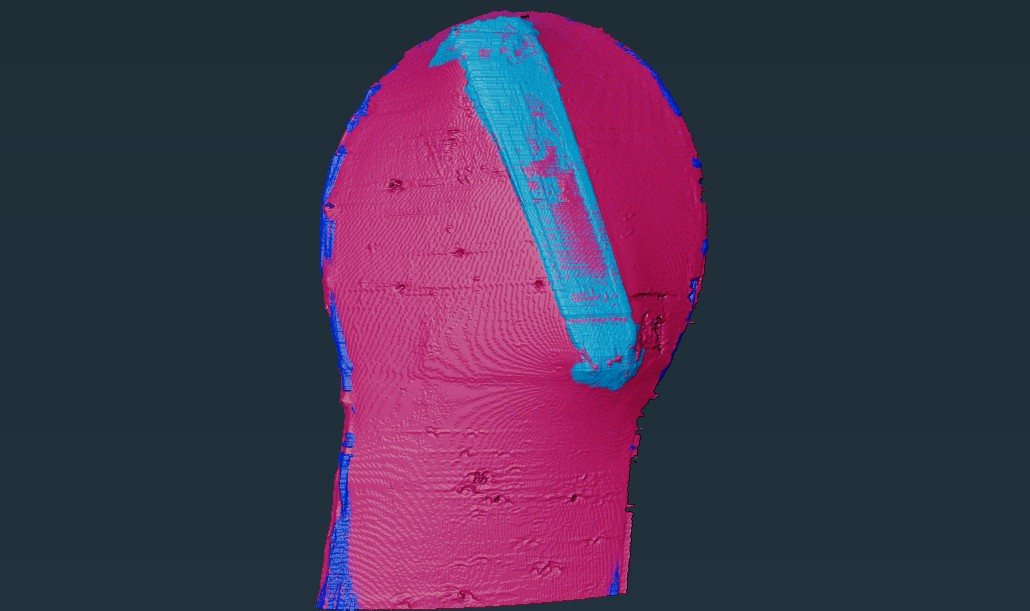
\includegraphics[height=7cm]{images/avizo_flats/tlys2.jpg}
    \end{tabular}
	\caption{Volume rendering in Avizo showing materials of crystal (light blue), liquor (pink), loop (dark blue): Thermolysin 1 (left) and Thermolysin 2 (right)}
 \label{tlys2}
\end{figure}
%\begin{figure}
	%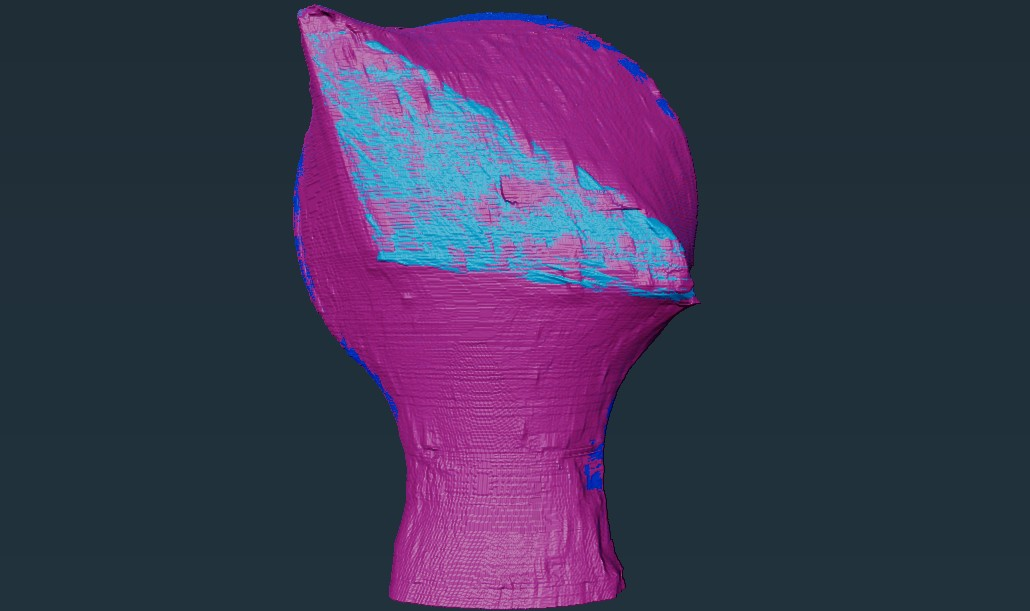
\includegraphics[width=0.5\textwidth]{images/avizo_flats/cas3_1118.jpg}
	%\caption{Volume rendering in Avizo:}
%\label{cas3}
%\end{figure}


\begin{figure}[h]
    \begin{tabular}{cc}
	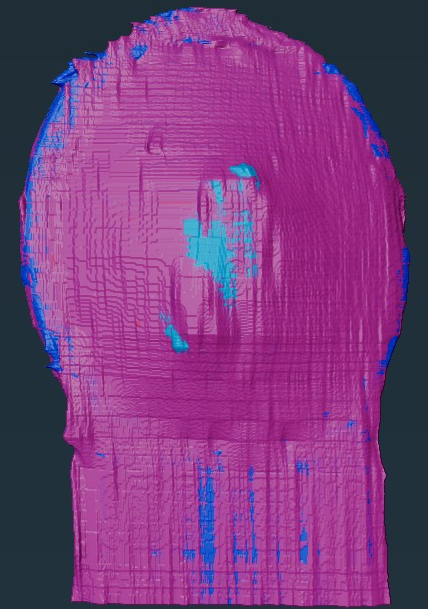
\includegraphics[height=7cm]{images/avizo_flats/ins_con.jpg} & 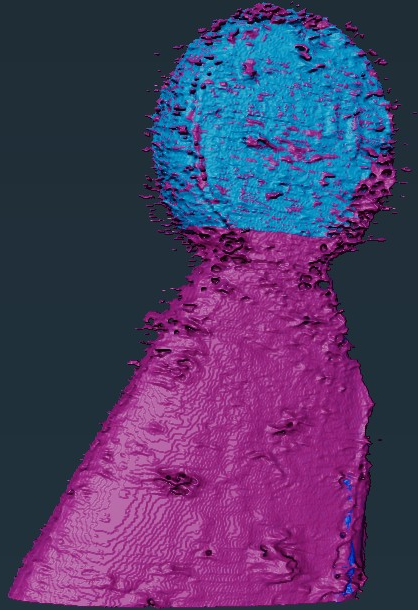
\includegraphics[height=7cm]{images/avizo_flats/ins_ls.jpg}
    \end{tabular}
	\caption{Volume rendering in Avizo showing materials of crystal (light blue), liquor (pink), loop (dark blue): Insulin control crystal (left) and laser-shaped crystal (right)}
 \label{avizo_insulin}
\end{figure}


\begin{figure}
    \begin{tabular}{cc}
	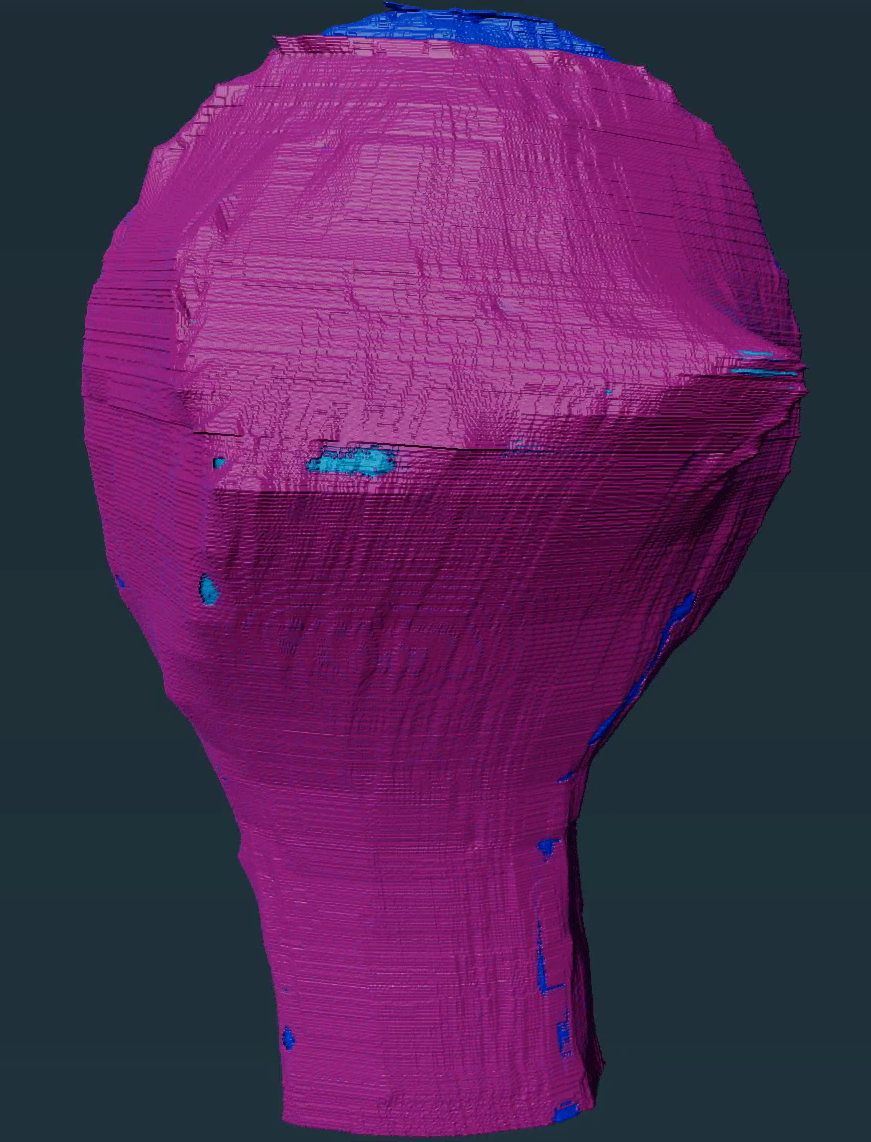
\includegraphics[height=7cm]{images/avizo_flats/prot_con.png} & 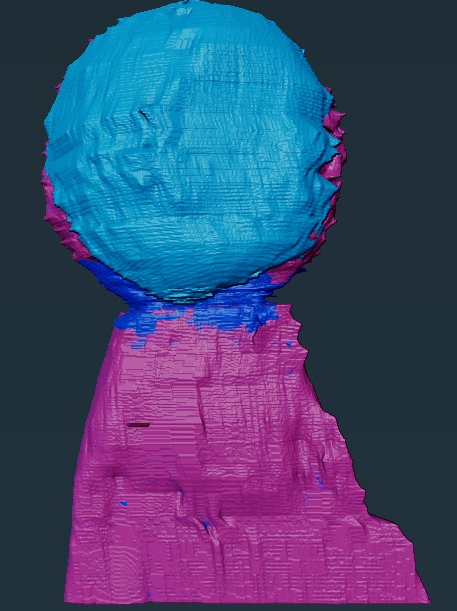
\includegraphics[height=7cm]{images/avizo_flats/prot_ls.jpg}
    \end{tabular}
    \caption{Volume rendering in Avizo showing materials of crystal (light blue), liquor (pink), loop (dark blue): Proteinase-K control crystal (left) and laser-shaped crystal (right)}
    \label{avizo_proteinasek}
\end{figure}


\onecolumn


\newpage
\subsection{B: Plots and Tables}
% Please add the following required packages to your document preamble:
% \usepackage{booktabs}
% \usepackage{multirow}
% \usepackage{graphicx}
\begin{table}[]
\resizebox{\textwidth}{!}{%
\begin{tabular}{@{}lllllll@{}}
\toprule
Crystal                    & Energy               & Processing symmetry group & N.o. datasets      & Transmission       & Kappa & Phi  \\ \midrule
\multirow{23}{*}{Thermolysin 1} & \multirow{7}{*}{3.0} & \multirow{4}{*}{P6122}     & \multirow{4}{*}{4} & \multirow{4}{*}{5}  & -25 & -100 \\
                           &                      &                           &                    &                    & -40   & 70   \\
                           &                      &                           &                    &                    & -35   & -70  \\
                           &                      &                           &                    &                    & 0     & 0    \\
                           &                      & \multirow{3}{*}{P1}       & \multirow{3}{*}{3} & \multirow{3}{*}{5} & -70   & 0    \\
                           &                      &                           &                    &                    & -70   & 120  \\
                           &                      &                           &                    &                    & -70   & -120 \\ \cmidrule(l){2-7} 
                           & \multirow{8}{*}{3.5} & \multirow{5}{*}{P6122}    & \multirow{5}{*}{5} & \multirow{5}{*}{1} & 0     & 0    \\
                           &                      &                           &                    &                    & -15   & 100  \\
                           &                      &                           &                    &                    & -25   & -100 \\
                           &                      &                           &                    &                    & -40   & 70   \\
                           &                      &                           &                    &                    & -35   & -70  \\
                           &                      & \multirow{3}{*}{P1}       & \multirow{3}{*}{3} & \multirow{3}{*}{1} & -70   & -120 \\
                           &                      &                           &                    &                    & -70   & 0    \\
                           &                      &                           &                    &                    & -70   & 120  \\ \cmidrule(l){2-7} 
                           & \multirow{8}{*}{3.8} & \multirow{5}{*}{P6122}    & \multirow{5}{*}{5} & \multirow{5}{*}{1} & 0     & 0    \\
                           &                      &                           &                    &                    & -15   & 100  \\
                           &                      &                           &                    &                    & -25   & -100 \\
                           &                      &                           &                    &                    & -40   & 70   \\
                           &                      &                           &                    &                    & -35   & -70  \\ \cmidrule(l){3-7} 
                           &                      & \multirow{3}{*}{P1}       & \multirow{3}{*}{3} & \multirow{3}{*}{1} & -70   & -120 \\
                           &                      &                           &                    &                    & -70   & 0    \\
                           &                      &                           &                    &                    & -70   & 120  \\ \midrule
\multirow{9}{*}{Thermolysin 2}  & \multirow{4}{*}{3.0} & \multirow{4}{*}{P6122, P1} & \multirow{4}{*}{4} & \multirow{4}{*}{20} & 0   & 0    \\
                           &                      &                           &                    &                    & -70   & -100 \\
                           &                      &                           &                    &                    & -70   & 0    \\
                           &                      &                           &                    &                    & -70   & 100  \\ \cmidrule(l){2-7} 
                                & \multirow{5}{*}{3.5} & \multirow{5}{*}{P6122, P1} & \multirow{5}{*}{5} & \multirow{5}{*}{15} & 0   & 0    \\
                           &                      &                           &                    &                    & -70   & -100 \\
                           &                      &                           &                    &                    & -70   & 0    \\
                           &                      &                           &                    &                    & -70   & 100  \\
                           &                      &                           &                    &                    & 0     & 0    \\ \midrule
Insulin 1                  & 3.0                  & I213                      & 1                  & 20                 & 0     & 0    \\ \midrule
Insulin 2                  & 3.0                  & I213                      & 1                  & 15                 & 0     & 0    \\ \midrule
Proteinase-K 1             & 3.0                  & P43212                    & 1                  & 20                 & 0     & 0    \\ \midrule
Proteinase-K 2             & 3.0                  & P43212                    & 1                  & 20                 & 0     & 0    \\ \midrule
\multirow{4}{*}{Thaumatin} & 3.0                  & \multirow{4}{*}{P41212}   & 1                  &                    & 0     & 0    \\
                           & 3.5                  &                           & 1                  &                    & 0     & 0    \\
                           & 4.0                  &                           & 1                  &                    & 0     & 0    \\
                           & 4.5                  &                           & 1                  &                    & 0     & 0    \\ \bottomrule
\end{tabular}%
}
\caption{Diffraction Data Collection Parameters; collected at beamline I23, Diamond Light Source, UK.}
\label{diffration_table}
\end{table}

%\caption{Diffraction Data Collection Parameters}







% Please add the following required packages to your document preamble:
% \usepackage{booktabs}
% \usepackage{multirow}
% \usepackage{graphicx}
% \usepackage[table,xcdraw]{xcolor}
% Beamer presentation requires \usepackage{colortbl} instead of \usepackage[table,xcdraw]{xcolor}
\begin{table}[h]
\resizebox{\textwidth}{!}{%
\begin{tabular}{@{}lllll@{}}
\toprule
Crystal                          & Energy & N.o. datasets & Exposure time (s per 0.2 deg) & Notes                          \\ \midrule
                                 & 3.0    & 4             & 0.35                          &                                \\
                                 & 3.5    & 5             & 0.25                          &                                \\
\multirow{-3}{*}{Thermolysin 1}  & 3.8    & 5             & 0.22                          &                                \\
                                 & 3.0    & 4             & 0.25                          &                                \\
\multirow{-2}{*}{Thermolysin 2}  & 3.5    & 5             & 0.3                           &                                \\
                                 & 3.0    & 1             & 0.3                           &                                \\
\multirow{-2}{*}{Insulin 1}      & 3.5    & 1             & 0.25                          & \multirow{-2}{*}{laser-shaped} \\
                                 & 3.0    & 1             & 0.3                           &                                \\
\multirow{-2}{*}{Insulin 2}      & 3.5    & 1             & 0.25                          & \multirow{-2}{*}{control}      \\
                                 & 3.0    & 1             & 0.3                           &                                \\
\multirow{-2}{*}{Proteinase-K 1} & 3.5    & 1             & 0.25                          & \multirow{-2}{*}{laser-shaped} \\
                                 & 3.0    & 1             & 0.3                           &                                \\
\multirow{-2}{*}{Proteinase-K 2} & 3.5    & 1             & 0.25                          & \multirow{-2}{*}{control}      \\
                                 & 2.4    & 2             & 0.35                          &                                \\
                                 & 3.0    & 2             & 0.3                           &                                \\
\multirow{-3}{*}{Lysozyme}       & 3.5    & 3             & 0.2                           &                                \\
                                 & 3.0    & 1             & 0.35                          &                                \\
                                 & 3.5    & 1             & 0.2                           &                                \\
                                 & 4.0    & 1             & 0.28                          &                                \\
\multirow{-4}{*}{Thaumatin}      & 4.5    & 1             & 0.18                          &       \\
\bottomrule
\end{tabular}%
}

\caption{Tomography Data Collection Parameters; collected using the goniometer at $\kappa$, $\phi$ = 0$\deg$, 0$\deg$ at the I23 endstation, Diamond Light Source, UK.}
\label{tomo_table}
\end{table}




% Please add the following required packages to your document preamble:
% \usepackage{booktabs}
% \usepackage{graphicx}
\begin{table}[h]
\resizebox{\textwidth}{!}{%
\begin{tabular}{@{}lllll@{}}
\toprule
Energy (eV) & Attenuation length (µm) & Theoretical coefficient (1/µm) & Experimental coefficient (1/µm) & Percentage Difference (\%) \\ \midrule
3000 & 60.3724 & 0.016564 & 0.01615  & -2.4973  \\
3500 & 95.0695 & 0.010519 & 0.010281 & -2.25611 \\
4000 & 141.783 & 0.007053 & 0.00696  & -1.32401 \\
4500 & 202.56  & 0.004937 & 0.00491  & -0.53778 \\
5000 & 279.179 & 0.003582 & 0.003625 & 1.215159 \\
6000 & 488.075 & 0.002049 & 0.002179 & 6.345384 \\ \bottomrule
\end{tabular}%
}
\caption{Experimentally calculated santovac absorption coefficients from AnACor at 50 \% material acceptance. Attenuation length calculated based on chemical formula \ce{C30H22O4} and density 1.195 \unit{\gram\per\cubic\cm} on the Center for X-Ray Optics \href{https://henke.lbl.gov/optical_constants/atten2.html}{X-ray Attenuation Length} platform.}
\label{santovac_table}
\end{table}


% Please add the following required packages to your document preamble:
% \usepackage{booktabs}
% \usepackage{graphicx}
\begin{table}[h]
\resizebox{\textwidth}{!}{%
\begin{tabular}{@{}lllll@{}}
\toprule
Energy (eV) & Attenuation length (µm) & Theoretical coefficient (1/µm) & Experimental coefficient (1/µm) & Percentage Difference (\%) \\ \midrule
3000 & 60.3724 & 0.016564 & 0.01615  & -2.4973  \\
3500 & 95.0695 & 0.010519 & 0.010281 & -2.25611 \\
4000 & 141.783 & 0.007053 & 0.00696  & -1.32401 \\
4500 & 202.56  & 0.004937 & 0.00491  & -0.53778 \\
5000 & 279.179 & 0.003582 & 0.003625 & 1.215159 \\
6000 & 488.075 & 0.002049 & 0.002179 & 6.345384 \\ \bottomrule
\end{tabular}%
}
\caption{Experimentally calculated ethylene glycol absorption coefficients from AnACor at 50 \% material acceptance. Attenuation length calculated based on chemical formula \ce{C2H6O2} and density 1.195 \unit{\gram\per\cubic\cm} on the Center for X-Ray Optics \href{https://henke.lbl.gov/optical_constants/atten2.html}{X-ray Attenuation Length} platform.}
\label{ethylene_table}
\end{table}



% Please add the following required packages to your document preamble:
% \usepackage{booktabs}
% \usepackage{multirow}
% \usepackage{graphicx}
% Please add the following required packages to your document preamble:
% \usepackage{booktabs}
% \usepackage{multirow}
% \usepackage{graphicx}
\begin{table}[h]
\resizebox{\textwidth}{!}{%
\begin{tabular}{@{}llllll@{}}
\toprule
\multirow{3}{*}{Atom, Energy} &
  \multirow{3}{*}{\begin{tabular}[c]{@{}l@{}}Theoretical f'\\ (used in Phenix.refine)\end{tabular}} &
  \multirow{3}{*}{Theoretical f"} &
  \multicolumn{3}{c}{Experimental f"} \\
                             &                            &                           & \multicolumn{1}{c}{AC} & \multicolumn{1}{c}{SH} & \multicolumn{1}{c}{ACSH} \\ \cmidrule(l){4-6} 
                             &                            &                           & \multicolumn{3}{c}{\% Difference}                                          \\ \midrule
\multirow{2}{*}{S, 3 \unit{keV}}    & \multirow{2}{*}{-0.75226}  & \multirow{2}{*}{3.059391} & 2.49912                & 2.45008                & 3.03552                  \\
                             &                            &                           & -18.3132               & -19.9161               & -0.78025                 \\ \midrule
\multirow{2}{*}{ZN, 3.0 \unit{keV}} & \multirow{2}{*}{3.56E-02}  & \multirow{2}{*}{3.764636} & 2.83766                & 2.36456                & 2.68316                  \\
                             &                            &                           & -24.6233               & -37.1902               & -28.7272                 \\ \midrule
\multirow{2}{*}{S, 3.5 \unit{keV}}  & \multirow{2}{*}{-8.16E-02} & \multirow{2}{*}{2.390438} & 2.21949                & 2.24339                & 2.42956                  \\
                             &                            &                           & -7.15133               & -6.15151               & 1.636604                 \\ \midrule
\multirow{2}{*}{ZN, 3.5 \unit{keV}}  & \multirow{2}{*}{-6.15E-02} & \multirow{2}{*}{2.912471} & 2.36736                & 2.1546                 & 2.62166                  \\
                             &                            &                           & -18.7164               & -26.0216               & -9.98503                 \\ \bottomrule
\end{tabular}%
}

\caption{Phenix Refinement on Thermolysin 2 reflection data, for sulphur and zinc at 3.0, 3.5 \unit{keV}.}
\label{phenix_table}
\end{table}



\begin{figure}[h]
    \centering
    \begin{tabular}{cc}
    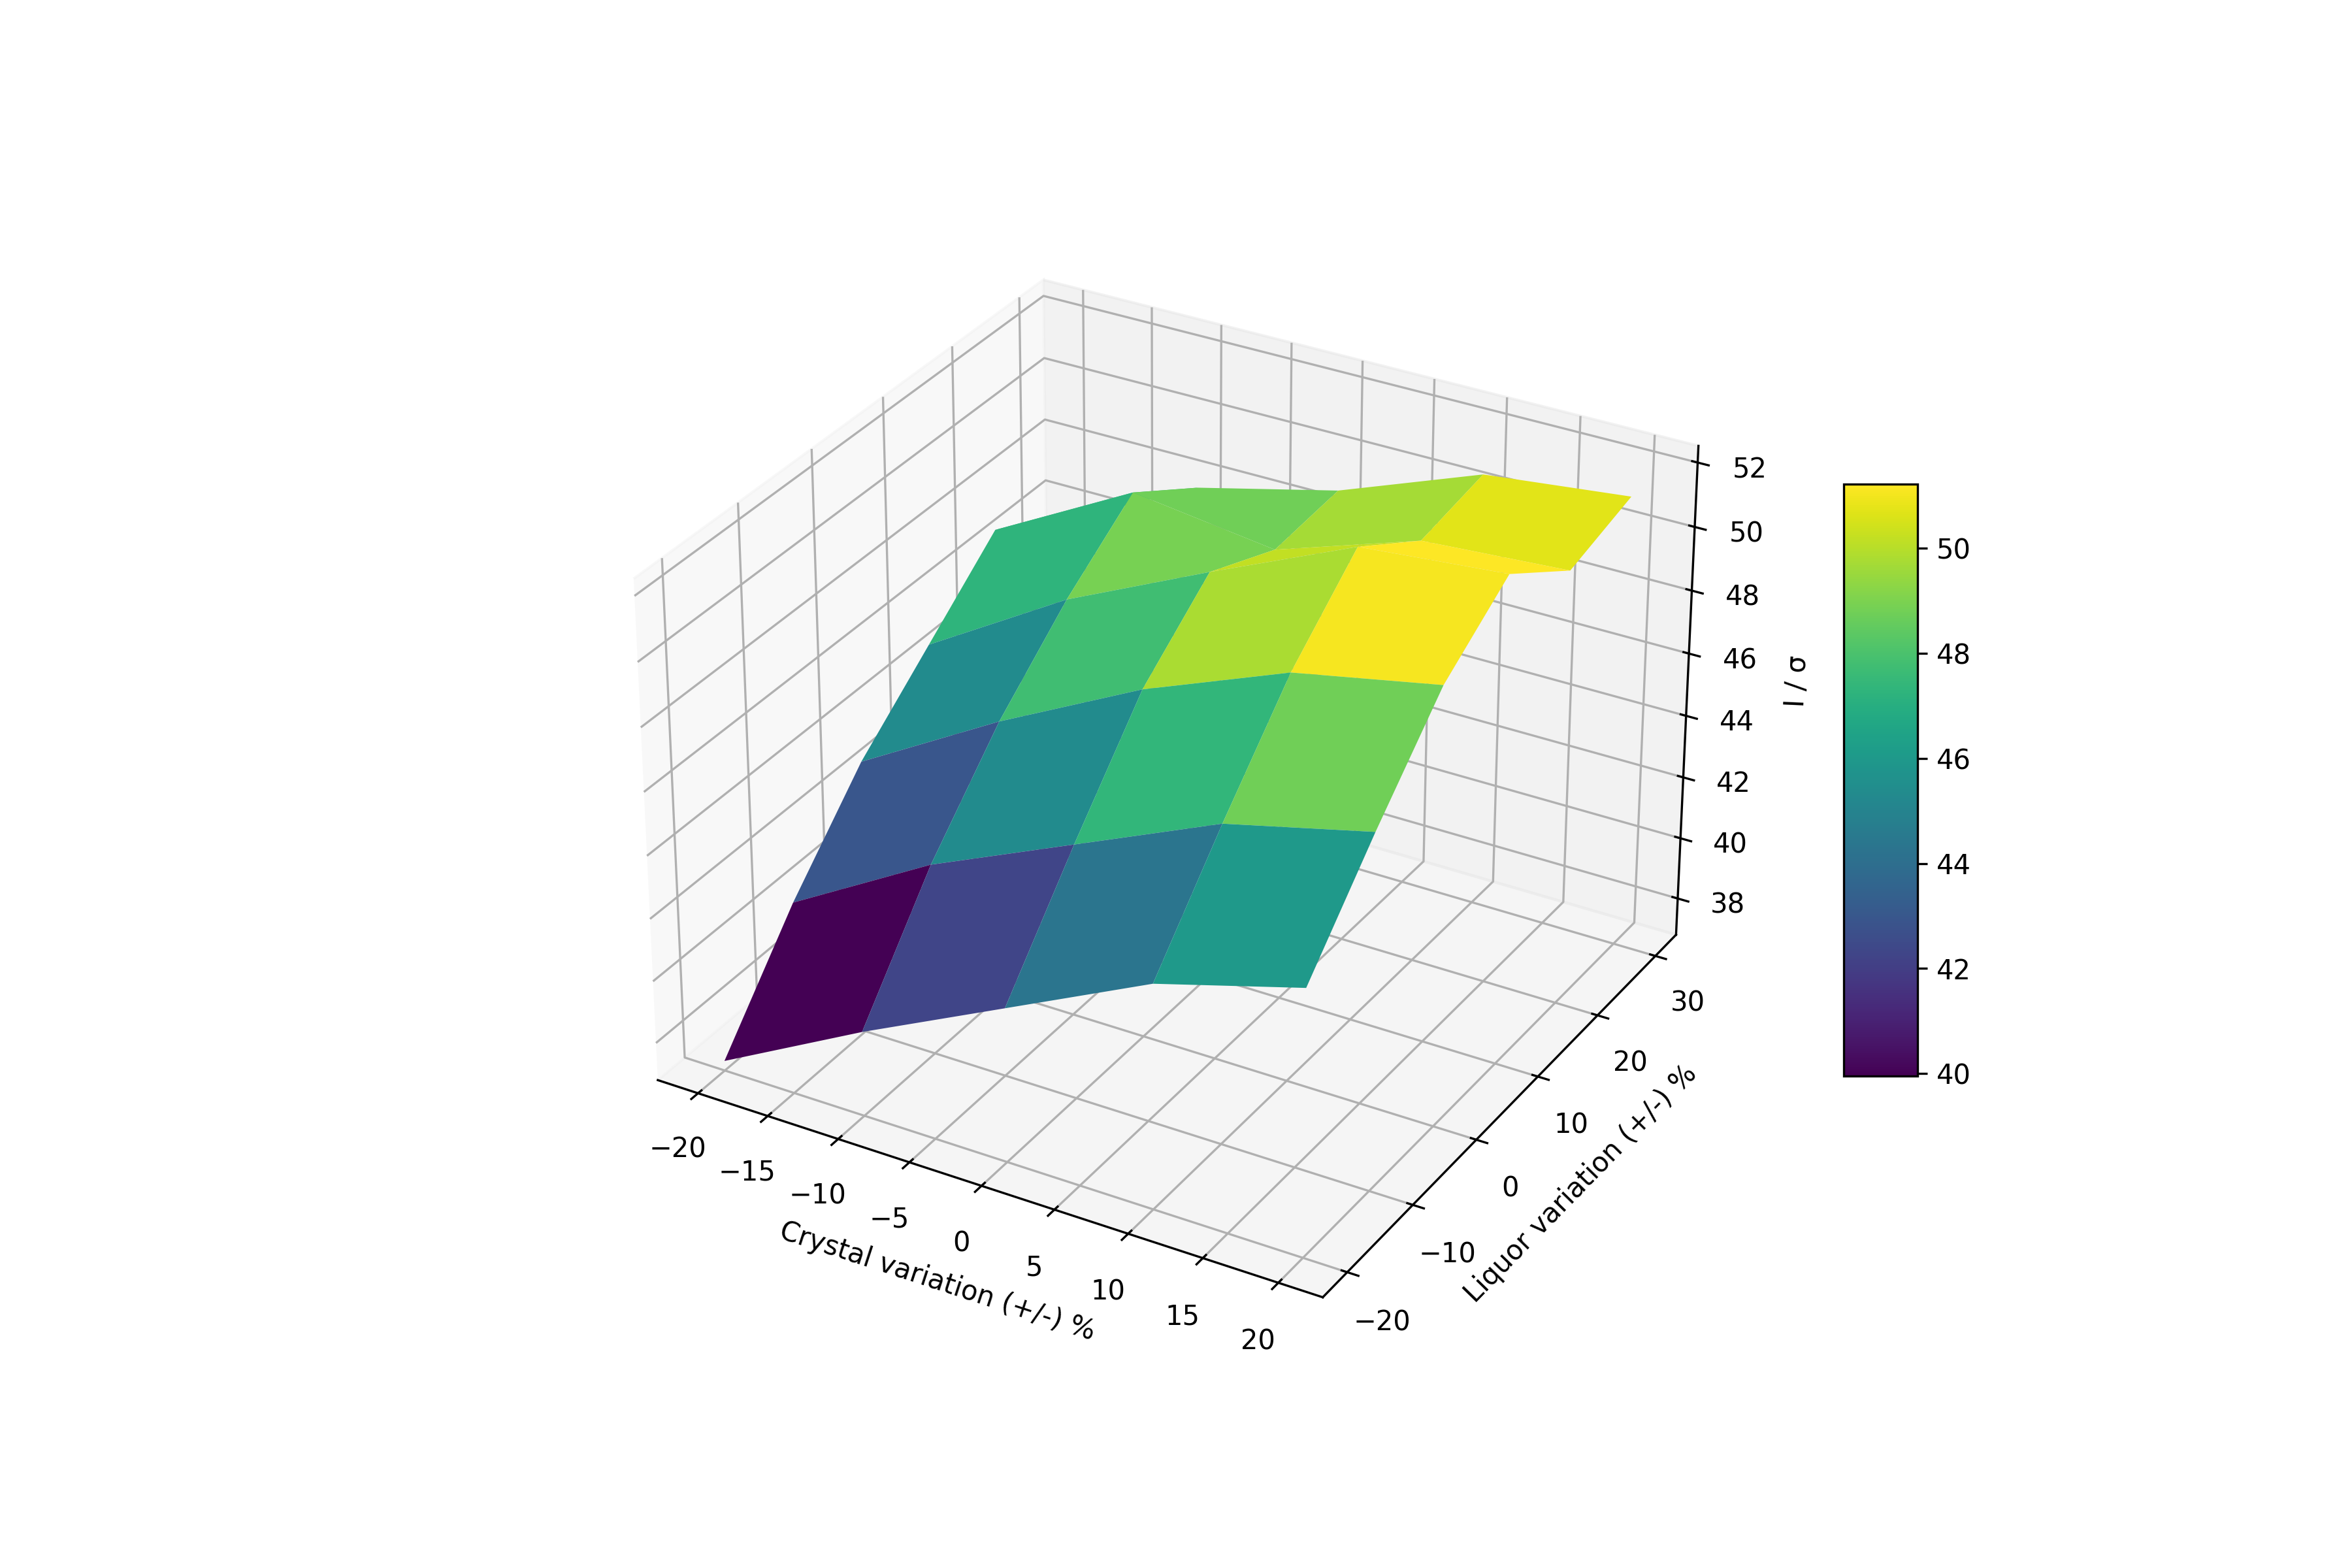
\includegraphics[width = 0.5\textwidth]{plots/exp0/cld_merged_Isig.png} & 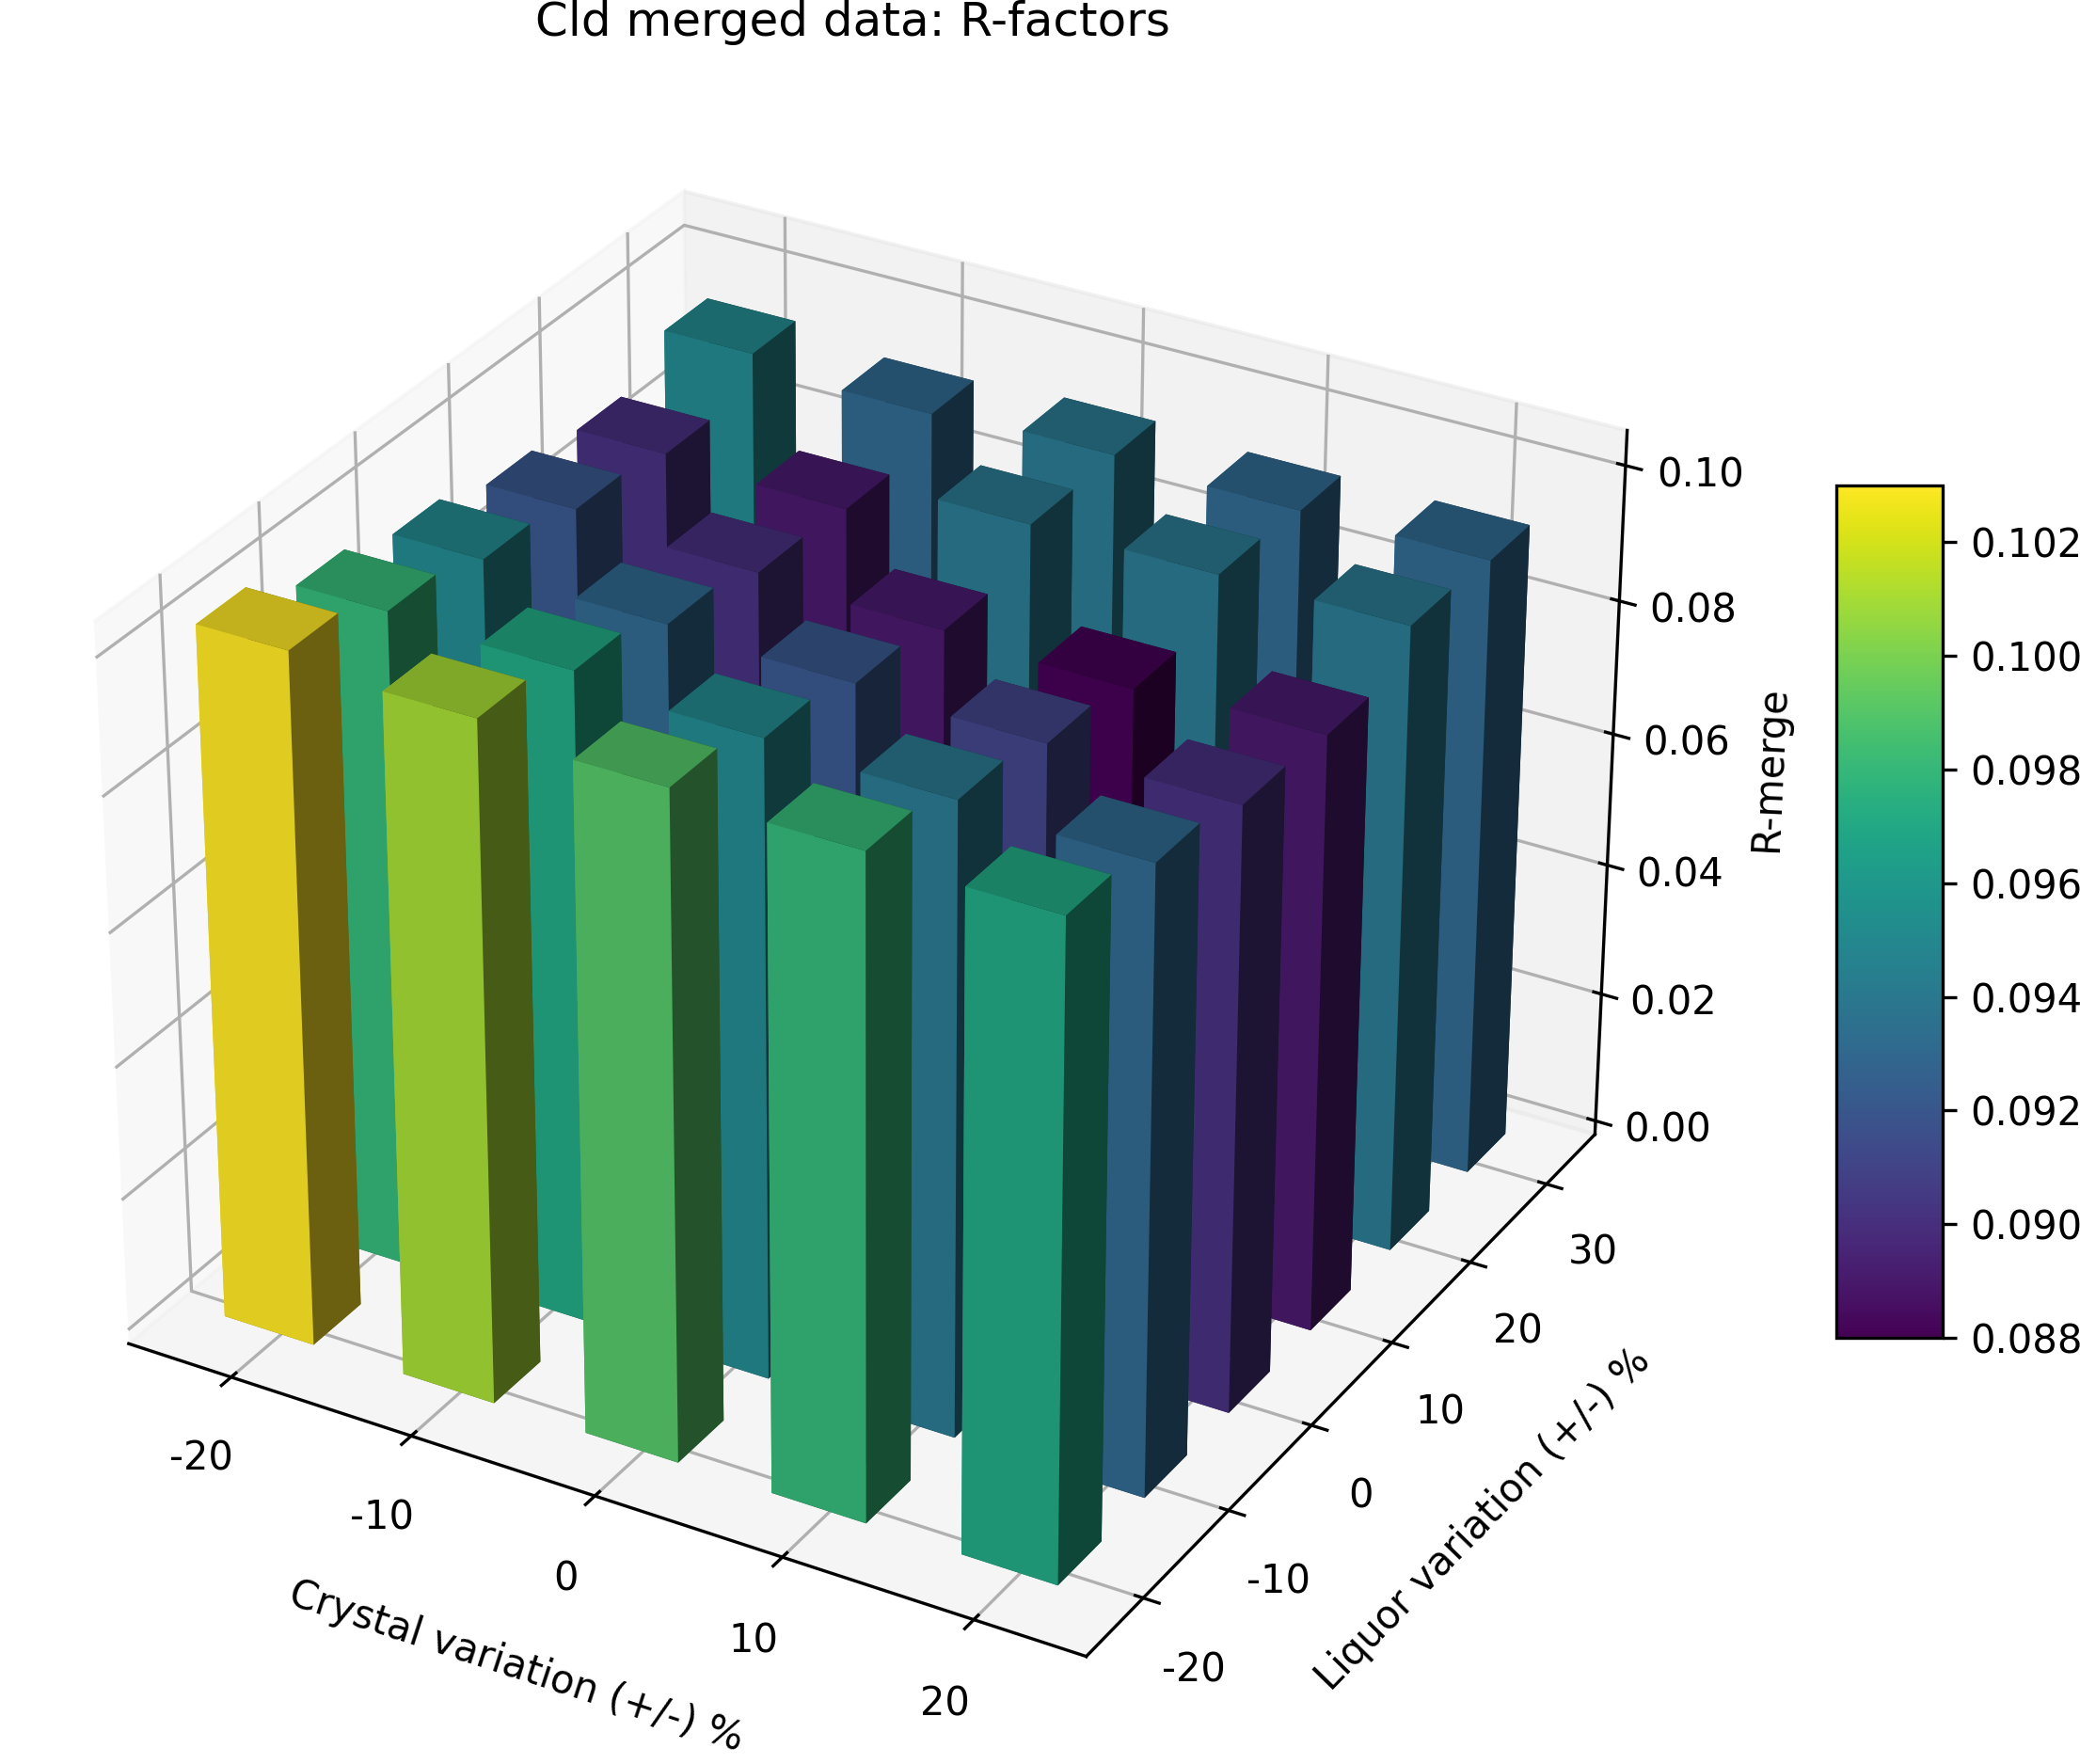
\includegraphics[trim={7.1cm 1cm 4.3cm 1cm},clip,width = 0.5\textwidth]{plots/exp0/cld_merged_rmerge.png} %[trim={5cm 0 5cm 0},clip]
    \end{tabular}
    \caption{Effects of varying the experimental Cld crystal and liquor absorption coefficients in Lu \textit{et al.} calculated by AnACor.}
    \label{fig:cld_stats}
\end{figure}

\begin{figure}[H]
    \centering
    \begin{tabular}{cc}
    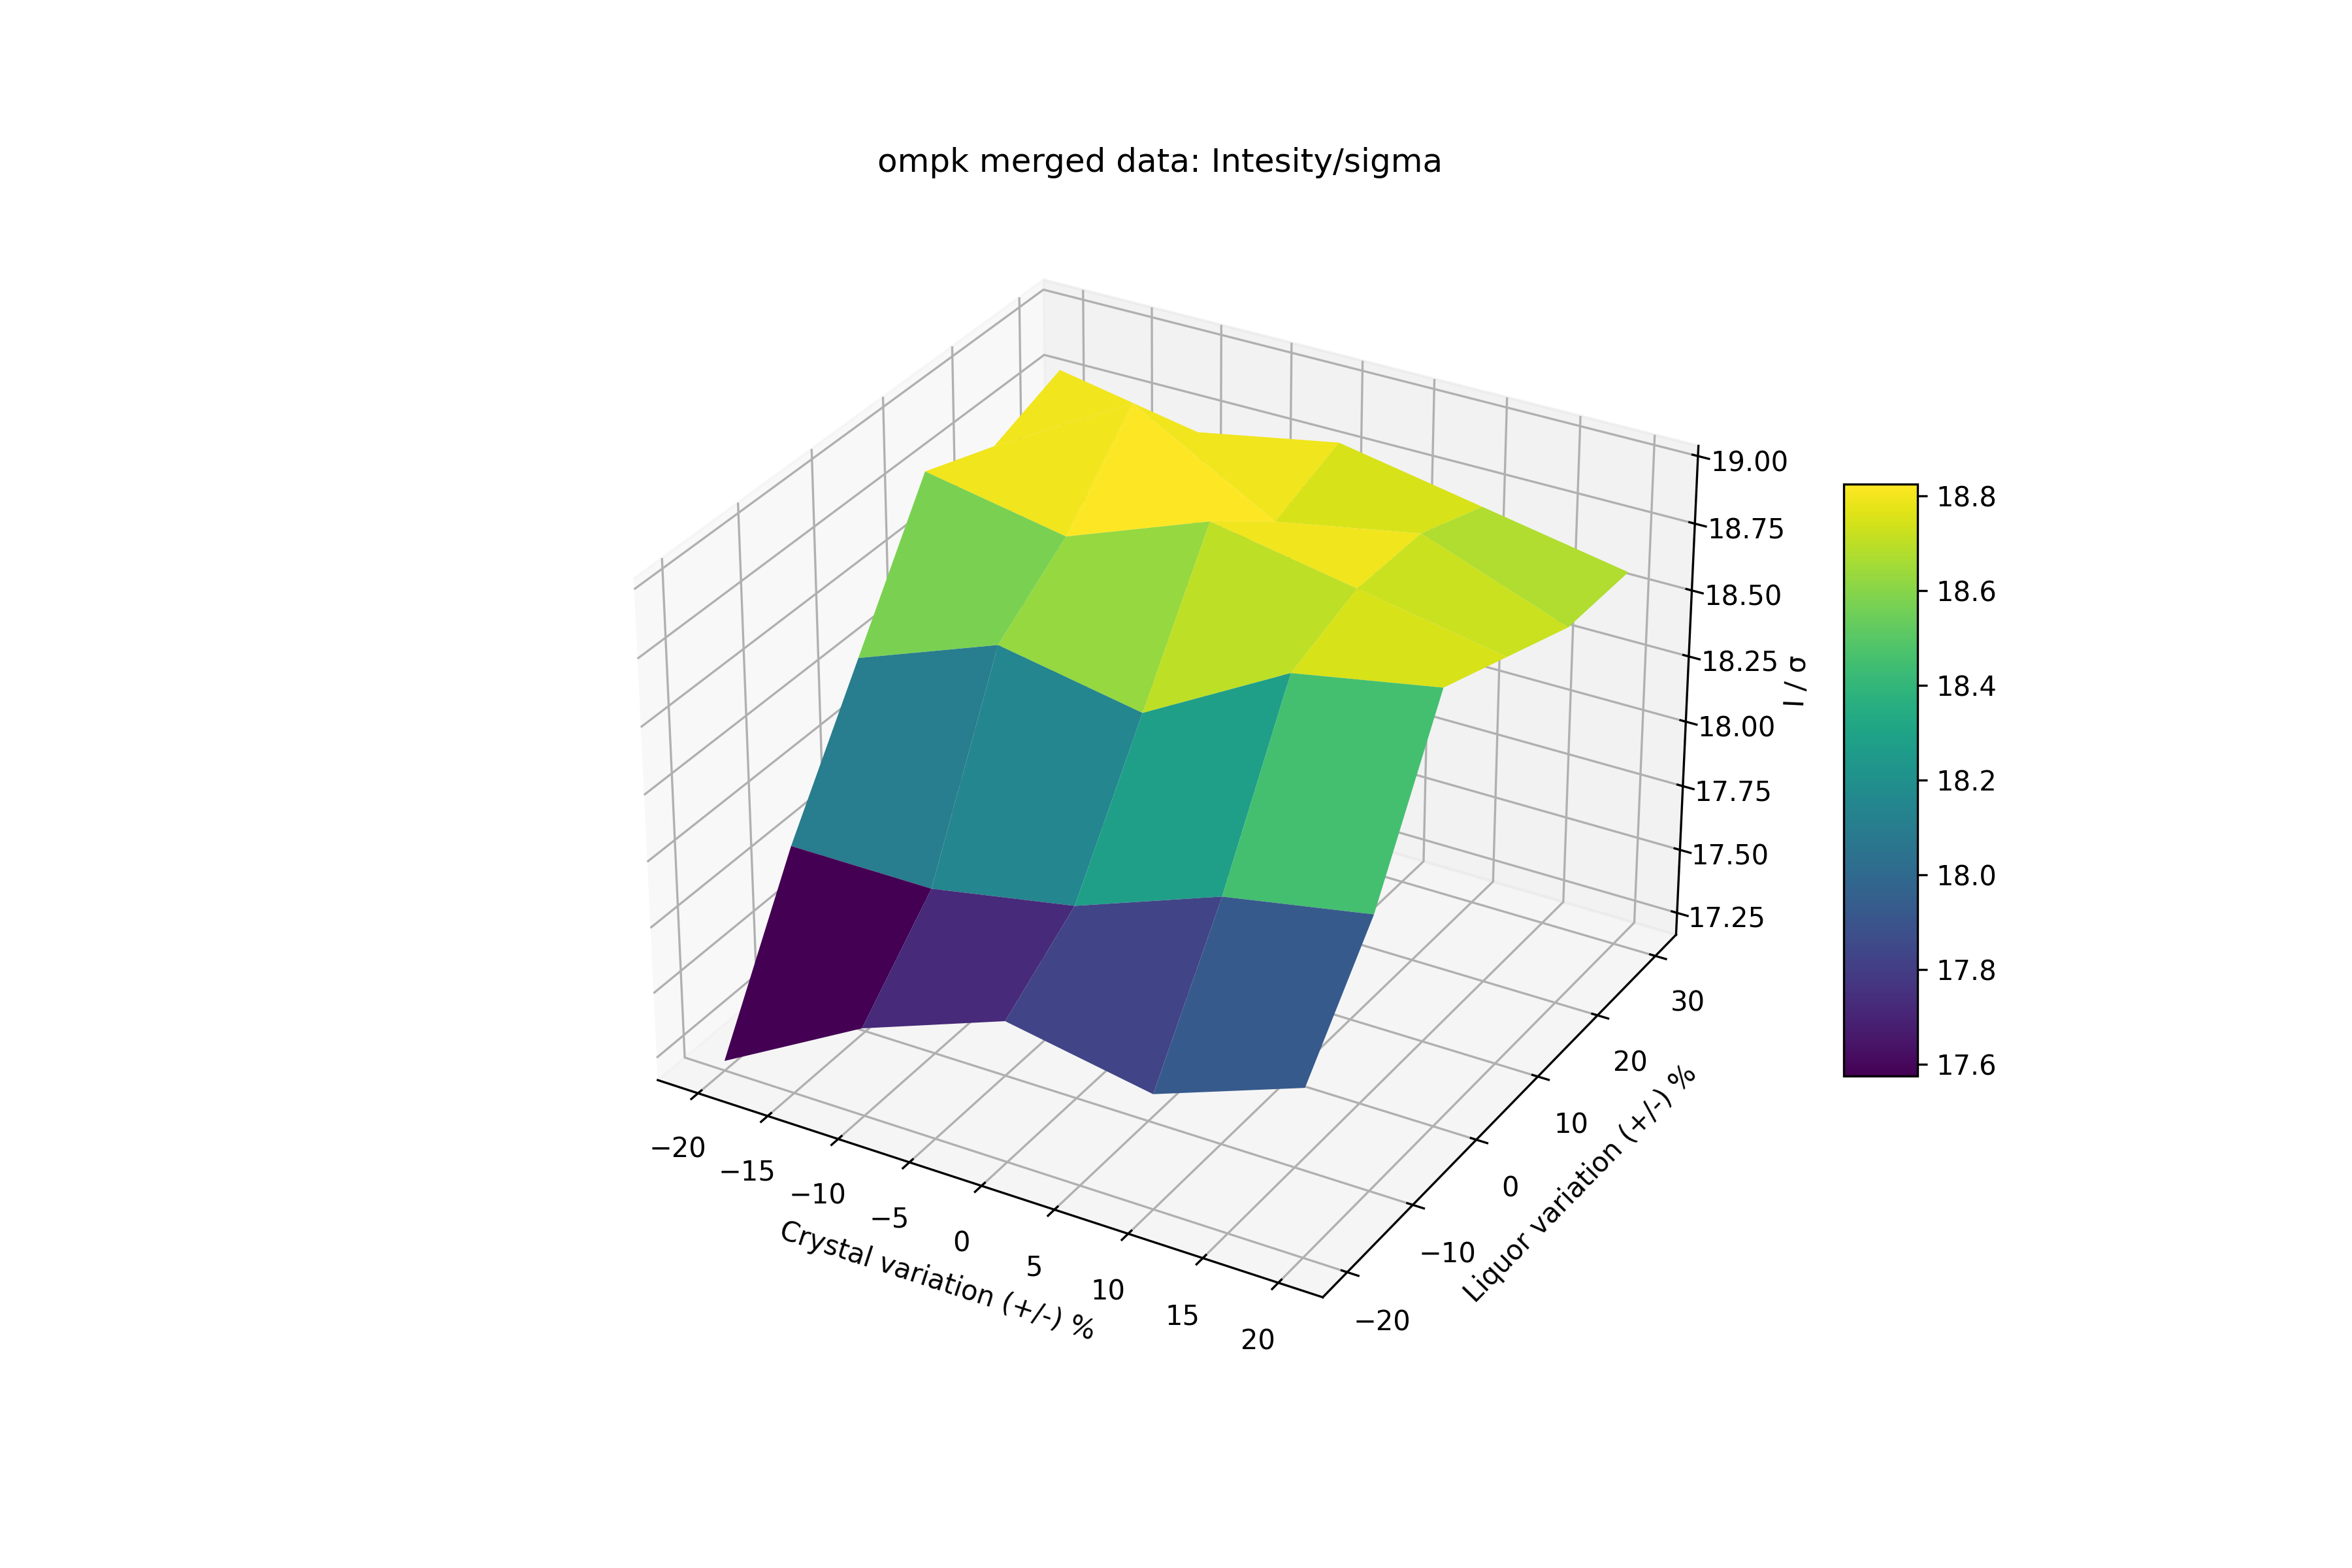
\includegraphics[width = 0.5\textwidth]{plots/exp0/ompk_merged_Isig.png} & 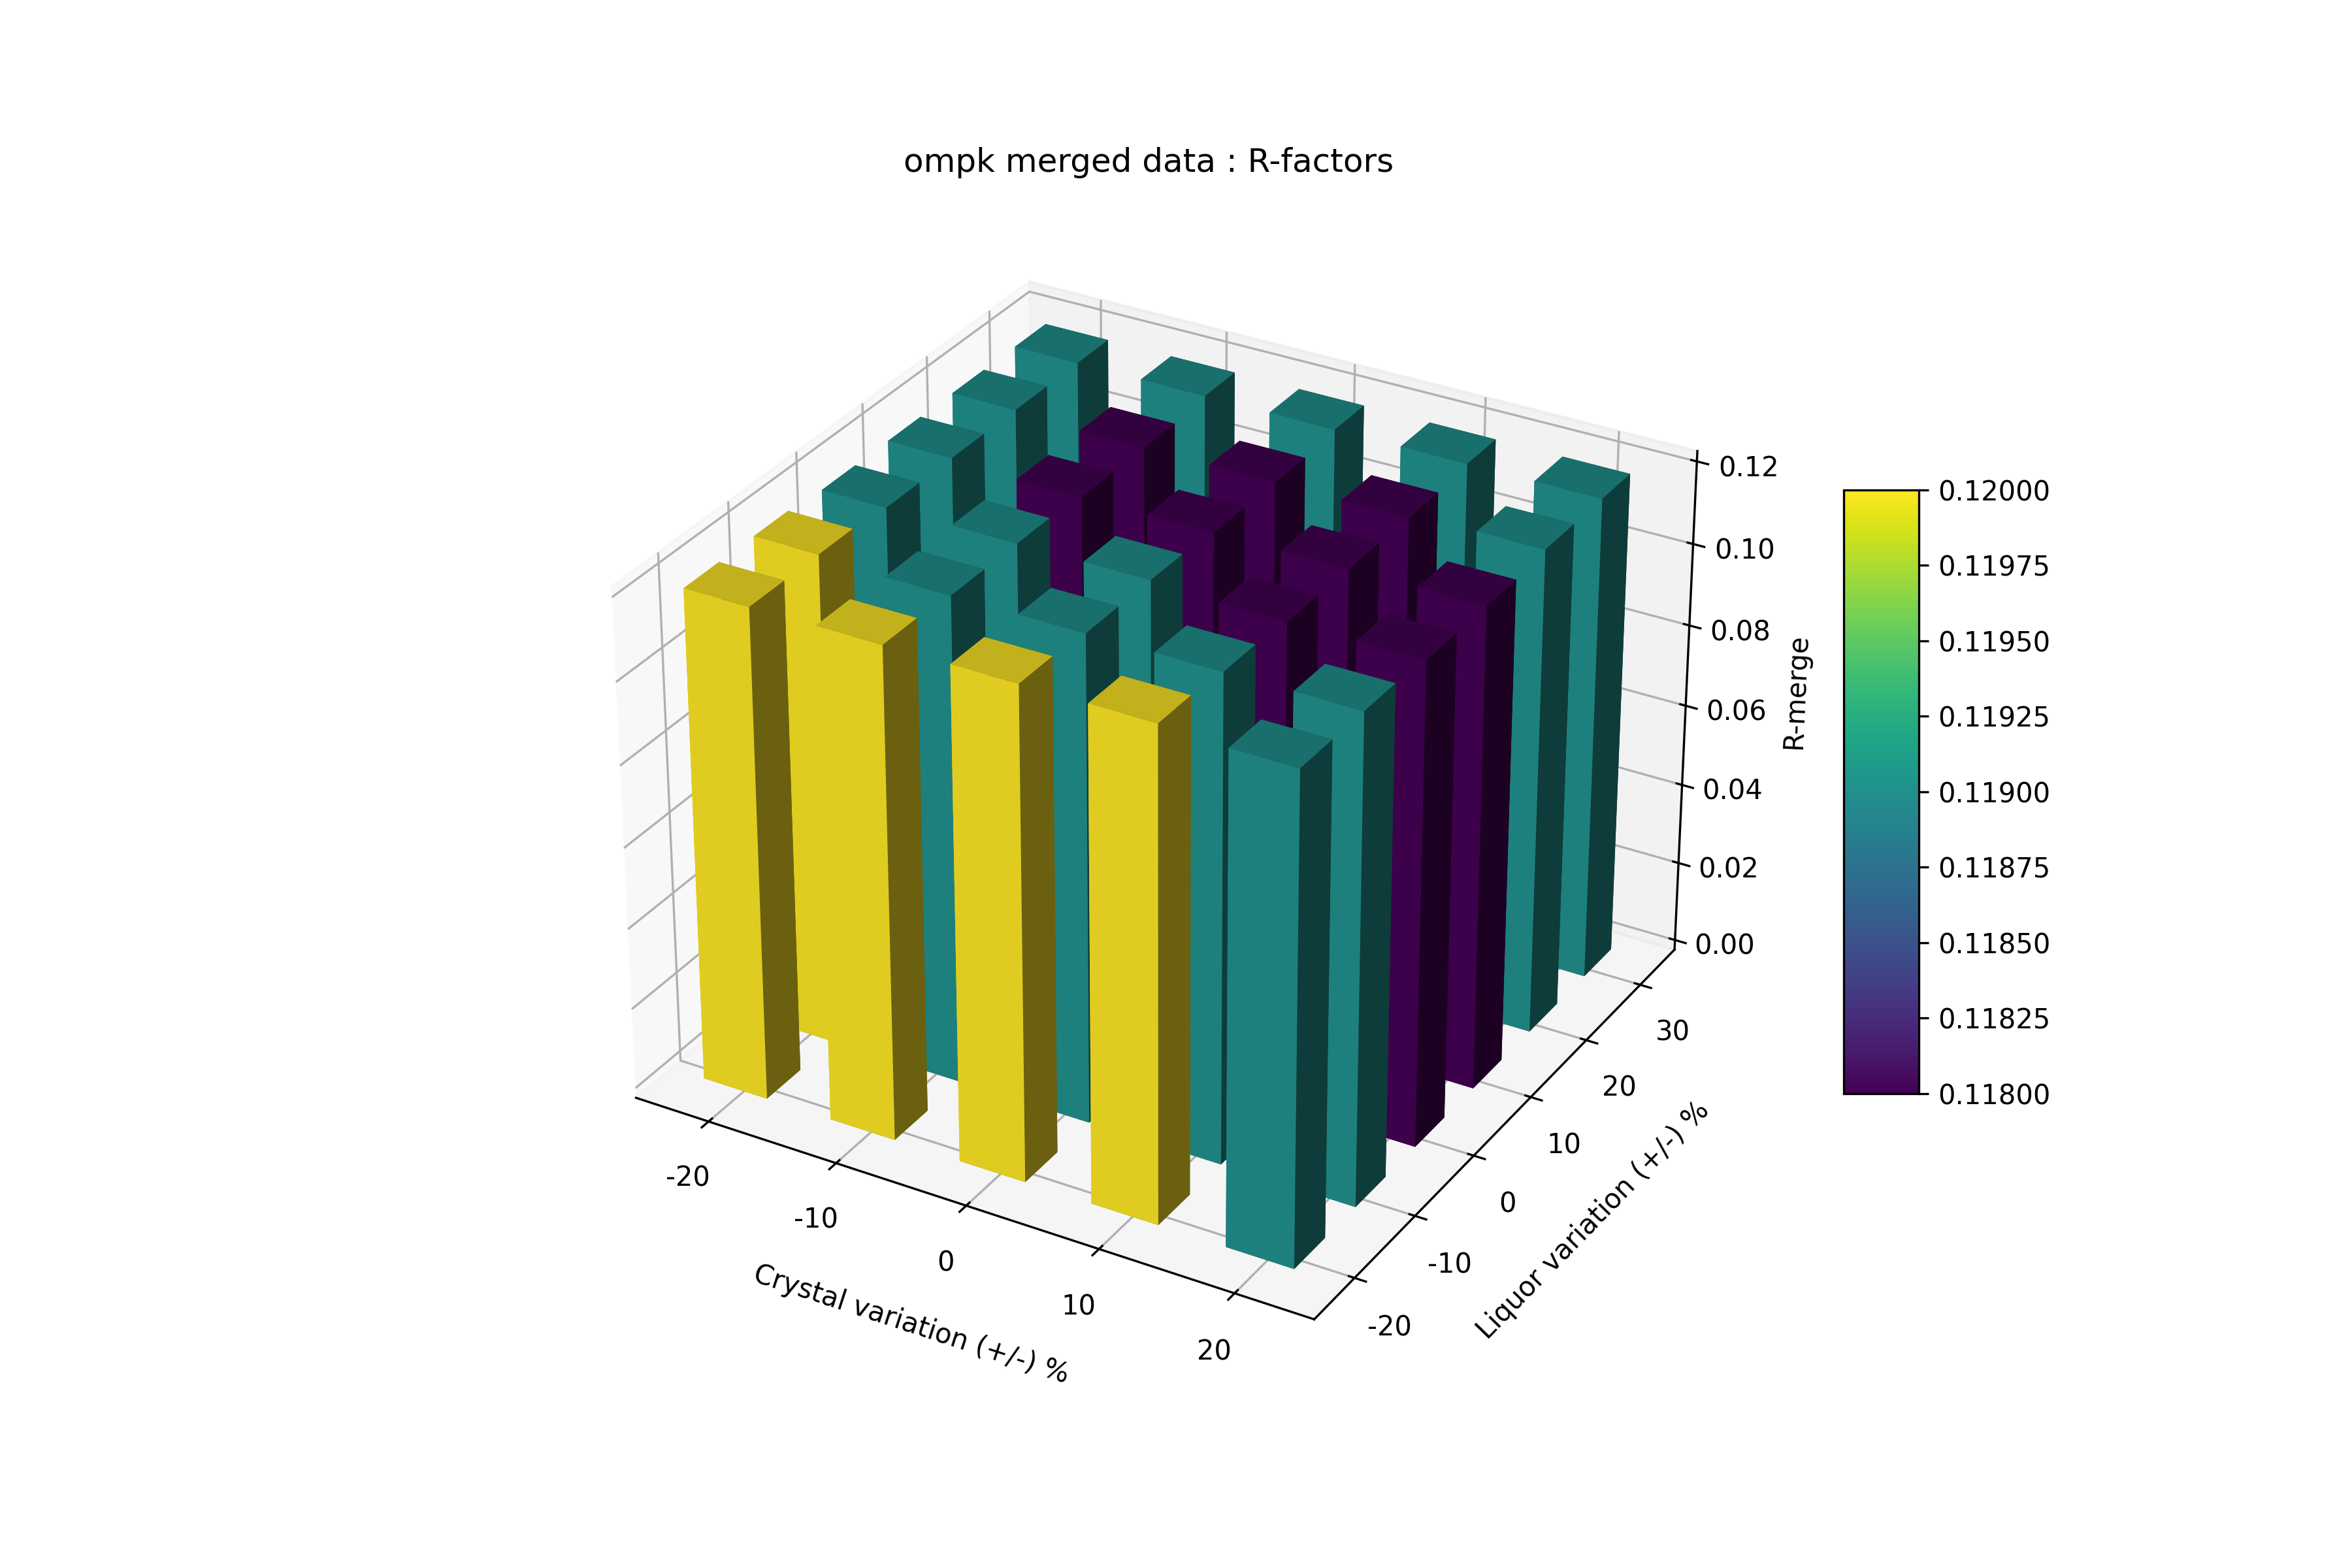
\includegraphics[width = 0.5\textwidth]{plots/exp0/ompk_merged_rmerge.png}
    \end{tabular}
    \caption{Effects of varying the experimental Ompk crystal and liquor absorption coefficients in Lu \textit{et al.} calculated by AnACor.}
    \label{fig:ompk_stats}
\end{figure}



\begin{figure}[h]
    \centering
    \begin{tabular}{cc}
    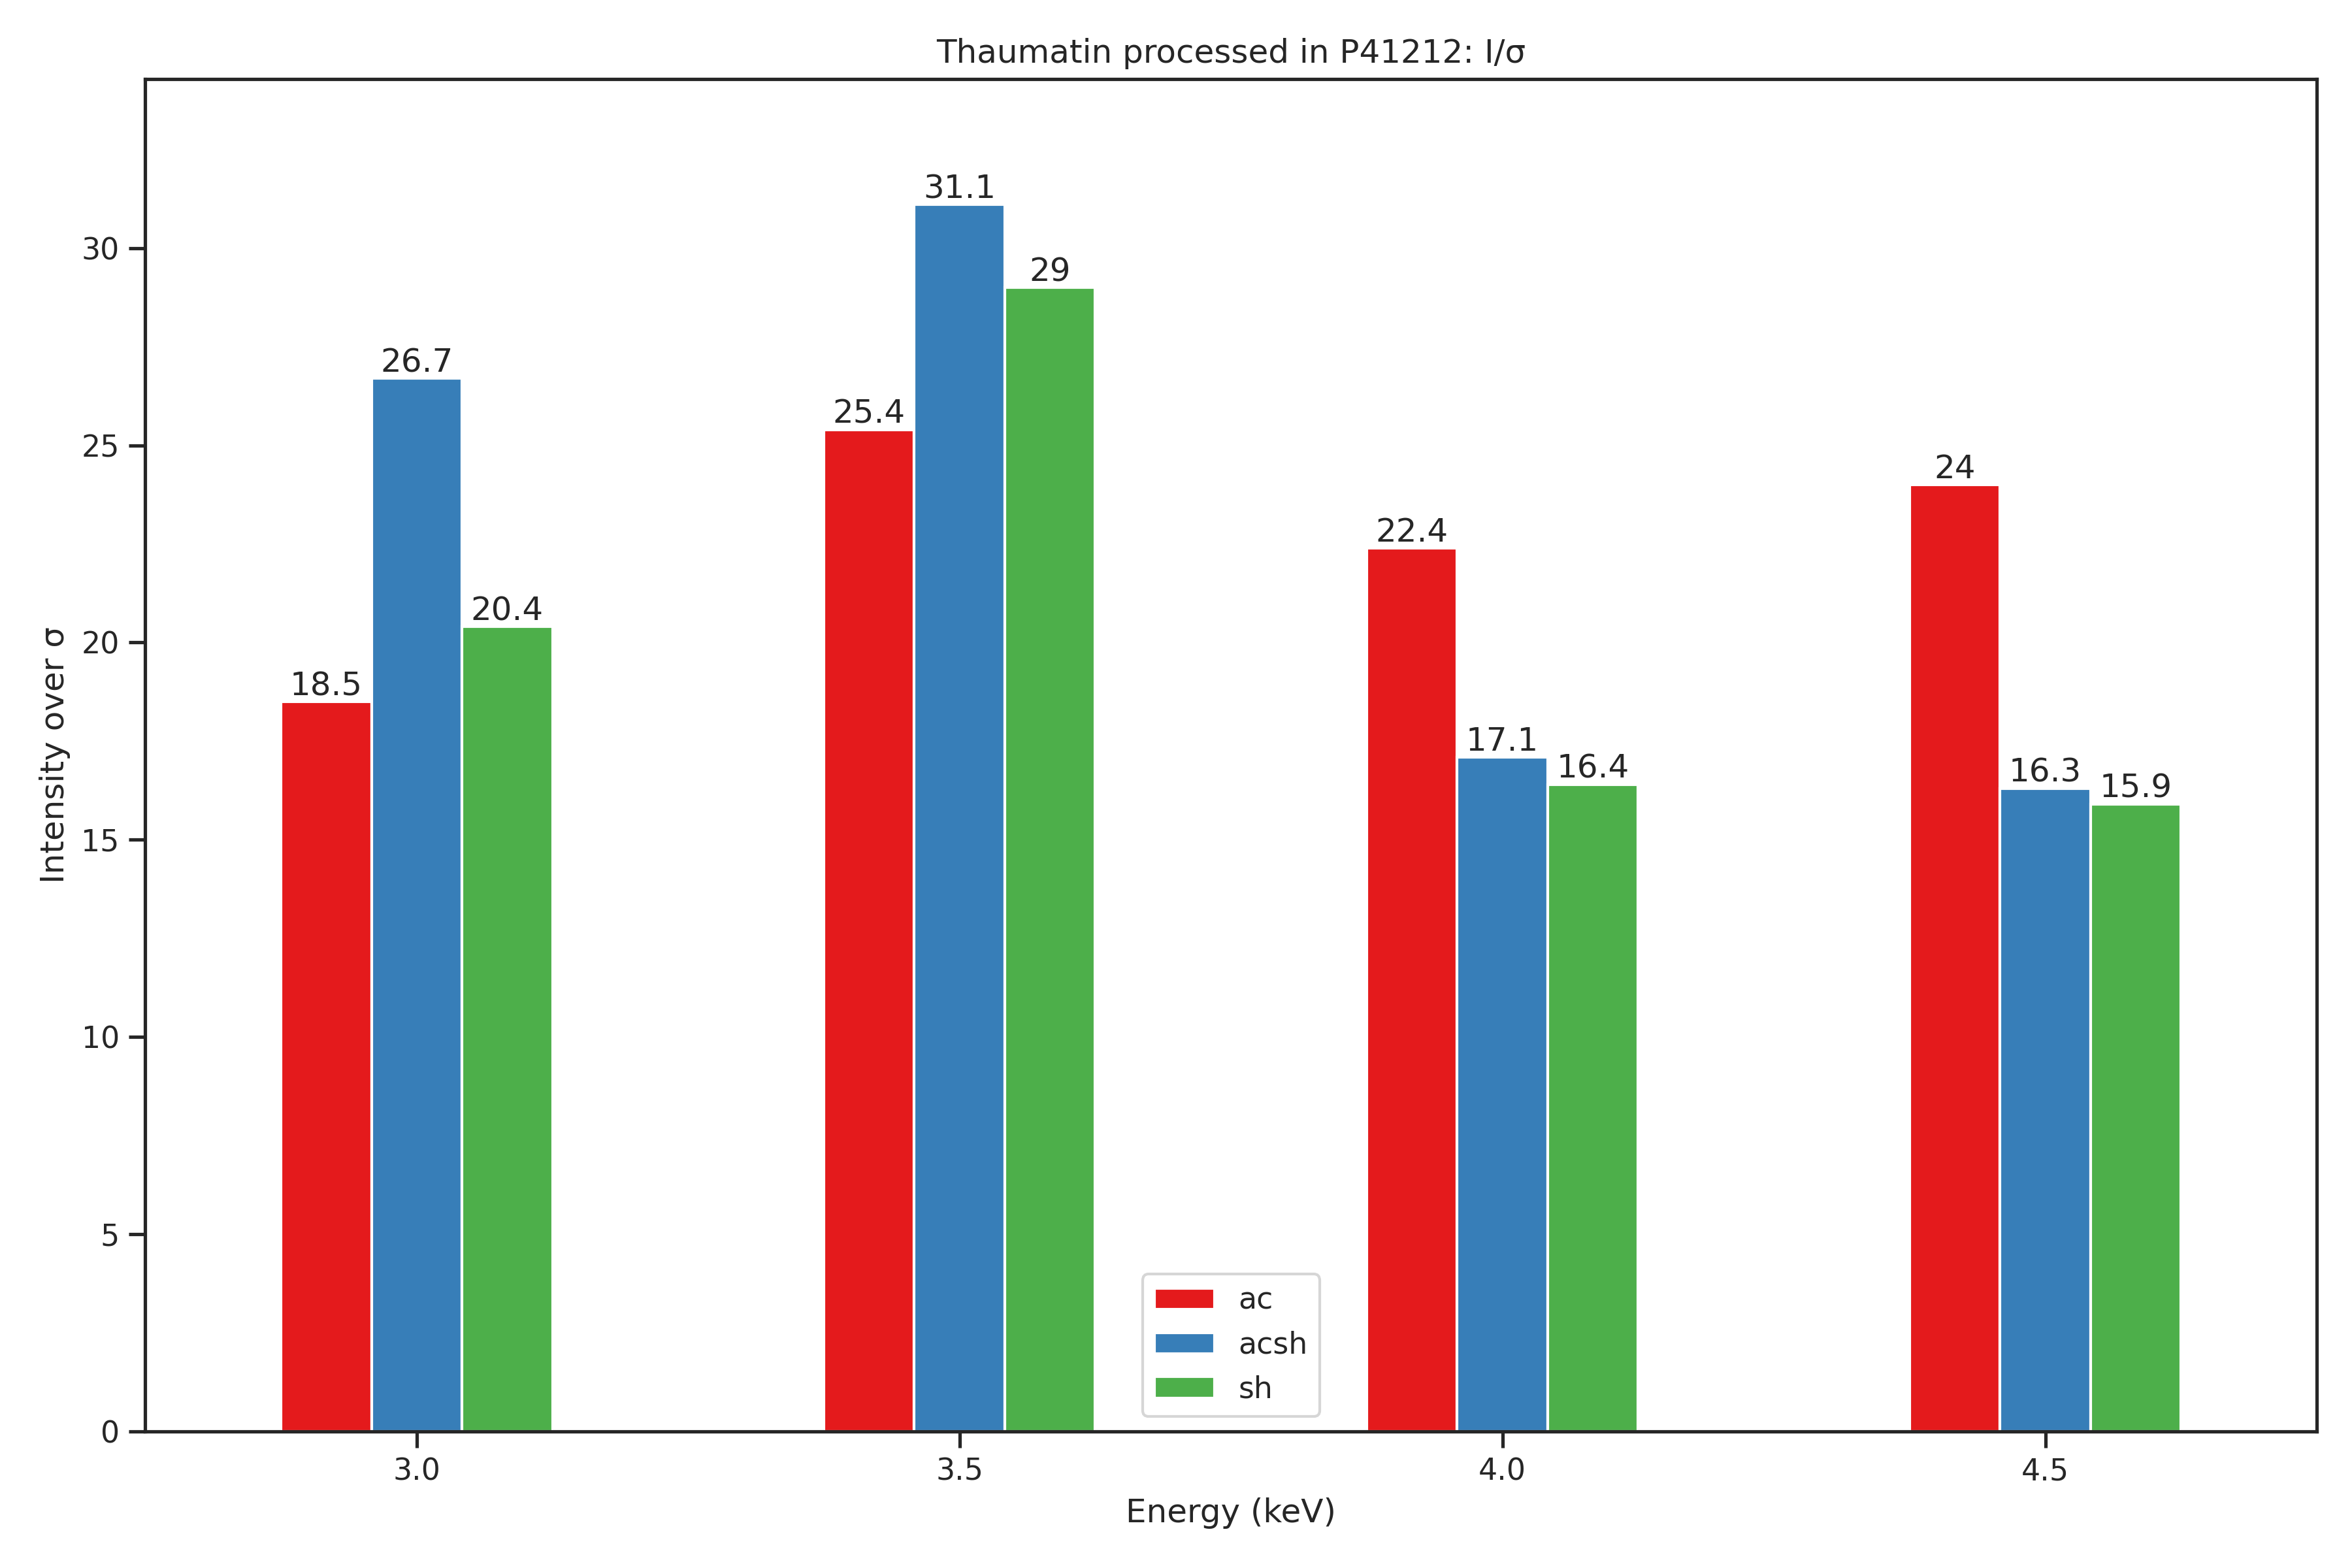
\includegraphics[width = 0.5\textwidth]{plots/exp0/thaum_Isig.png} & 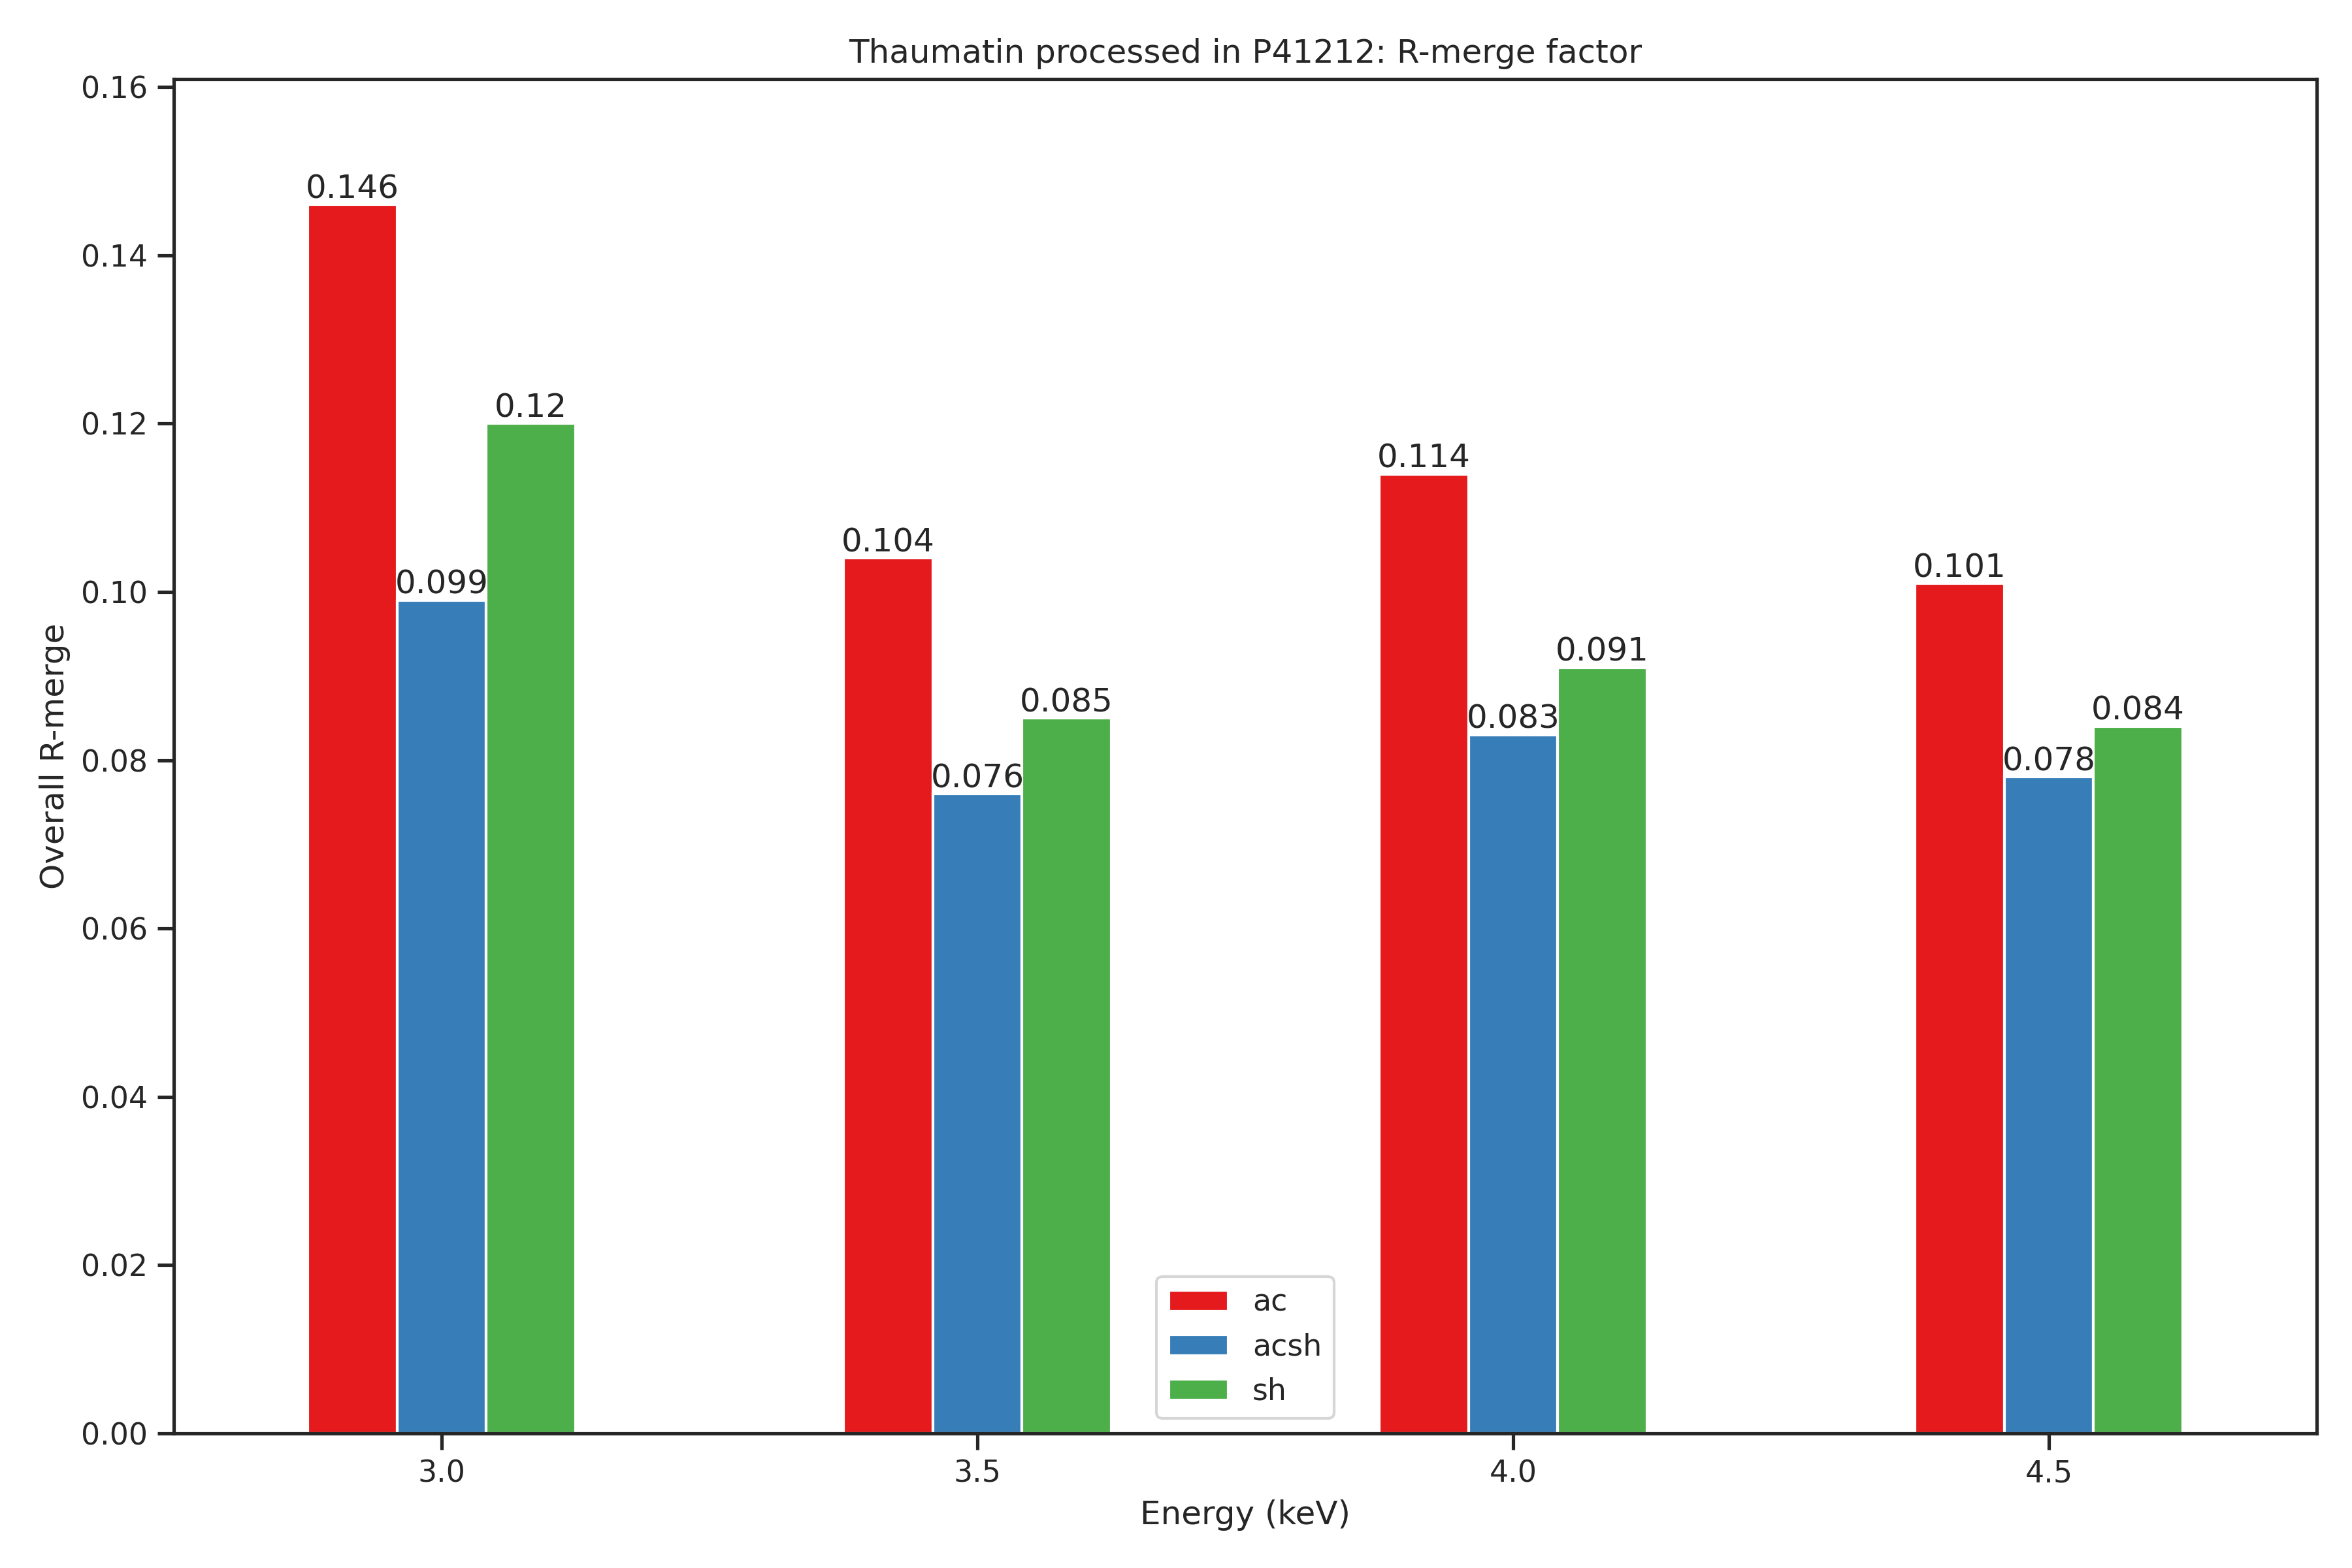
\includegraphics[width = 0.5\textwidth]{plots/exp0/thaum_rmerges.png}
    \end{tabular}
    \caption{Merging statistics for thaumatin crystal.}
    \label{fig:thaum1_stats}
\end{figure}


\newpage
%\section{Plots}

% TLYS 9 ANODE PEAKS
\begin{figure}
    \centering
    \begin{tabular}{cc}
        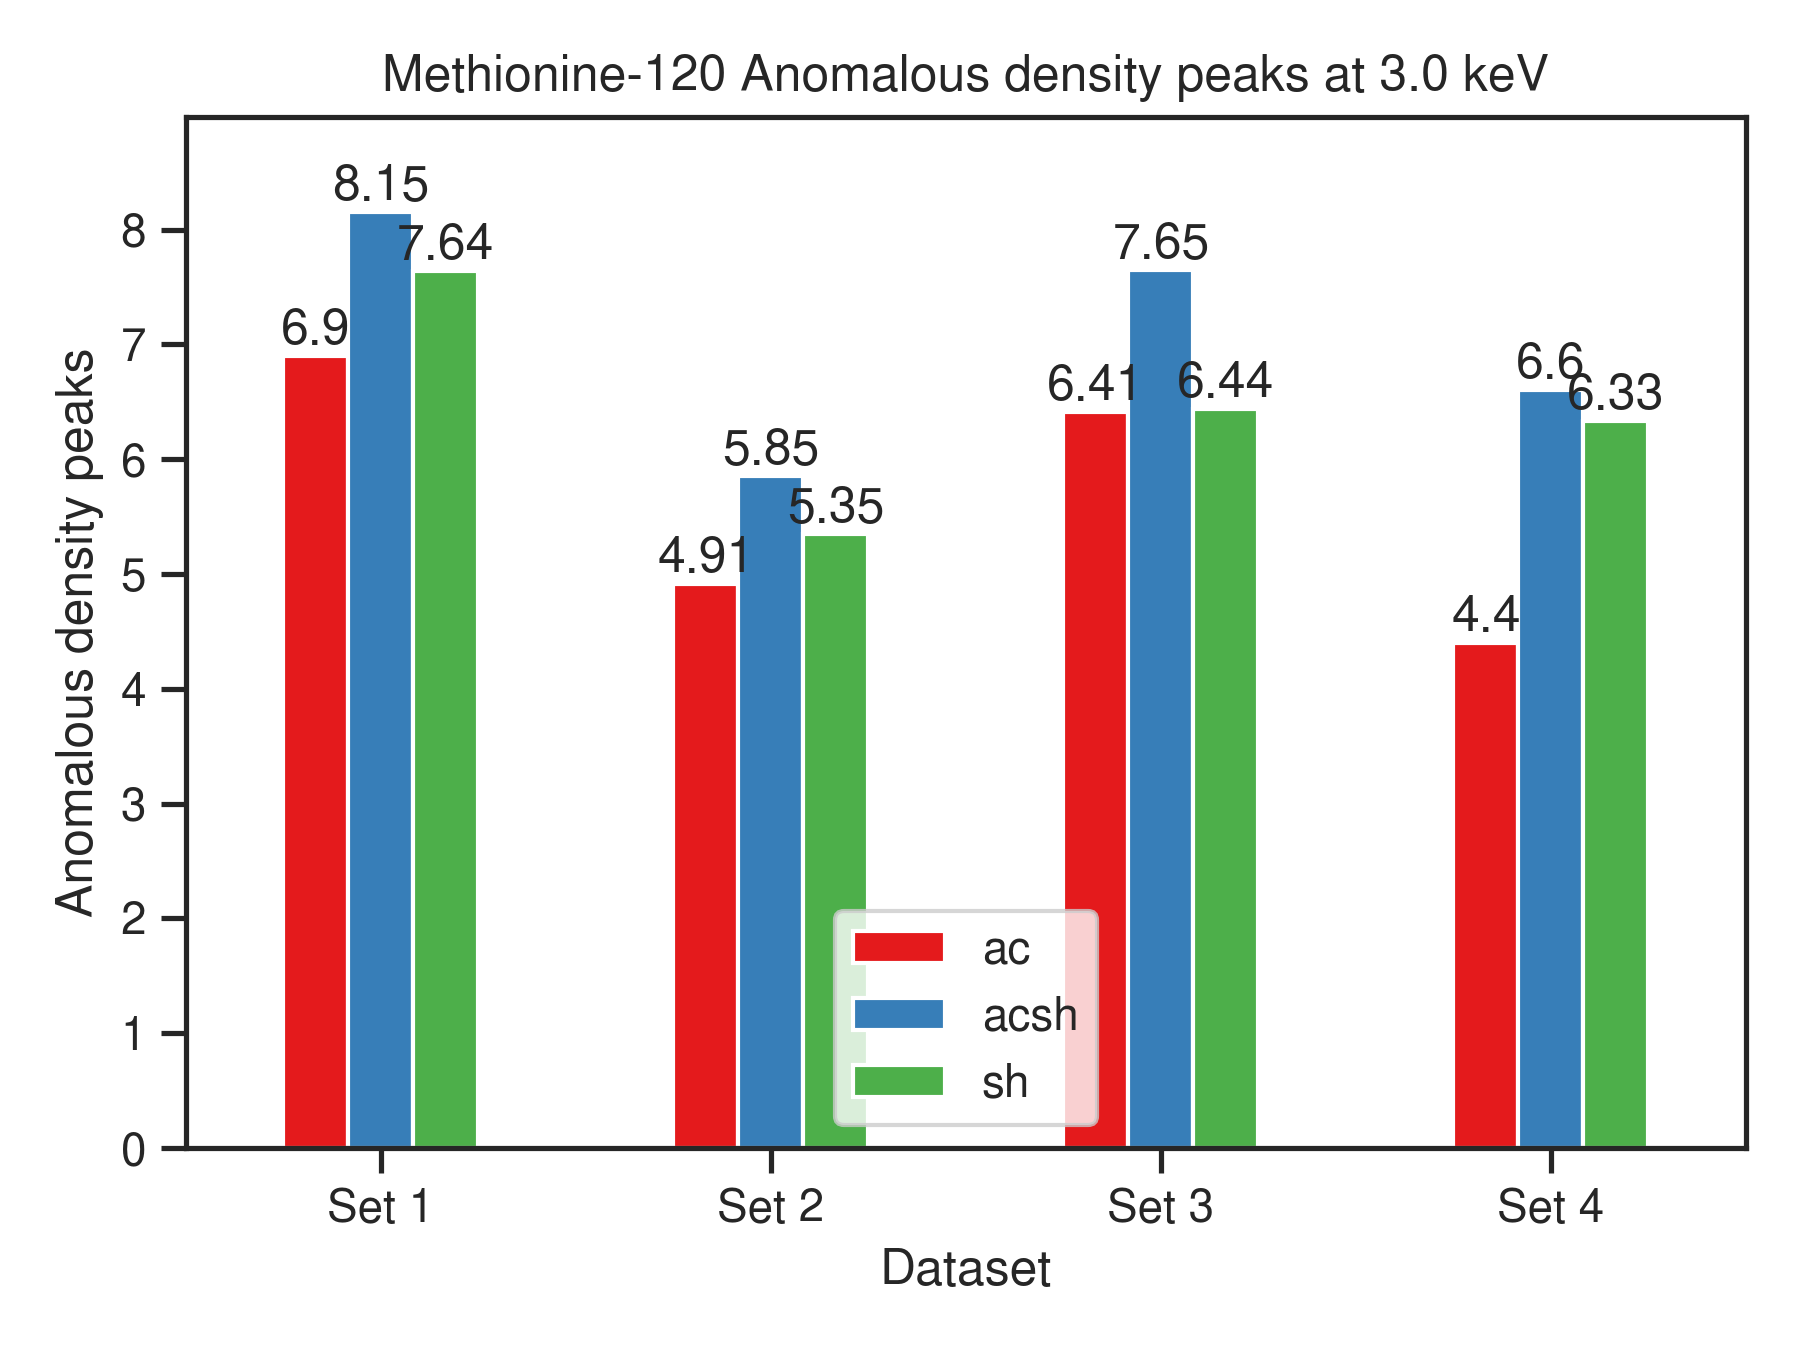
\includegraphics[width = 0.5\textwidth]{plots/exp1/tlys_9_P6122/peaks/3p0_met120_peaks.png} & 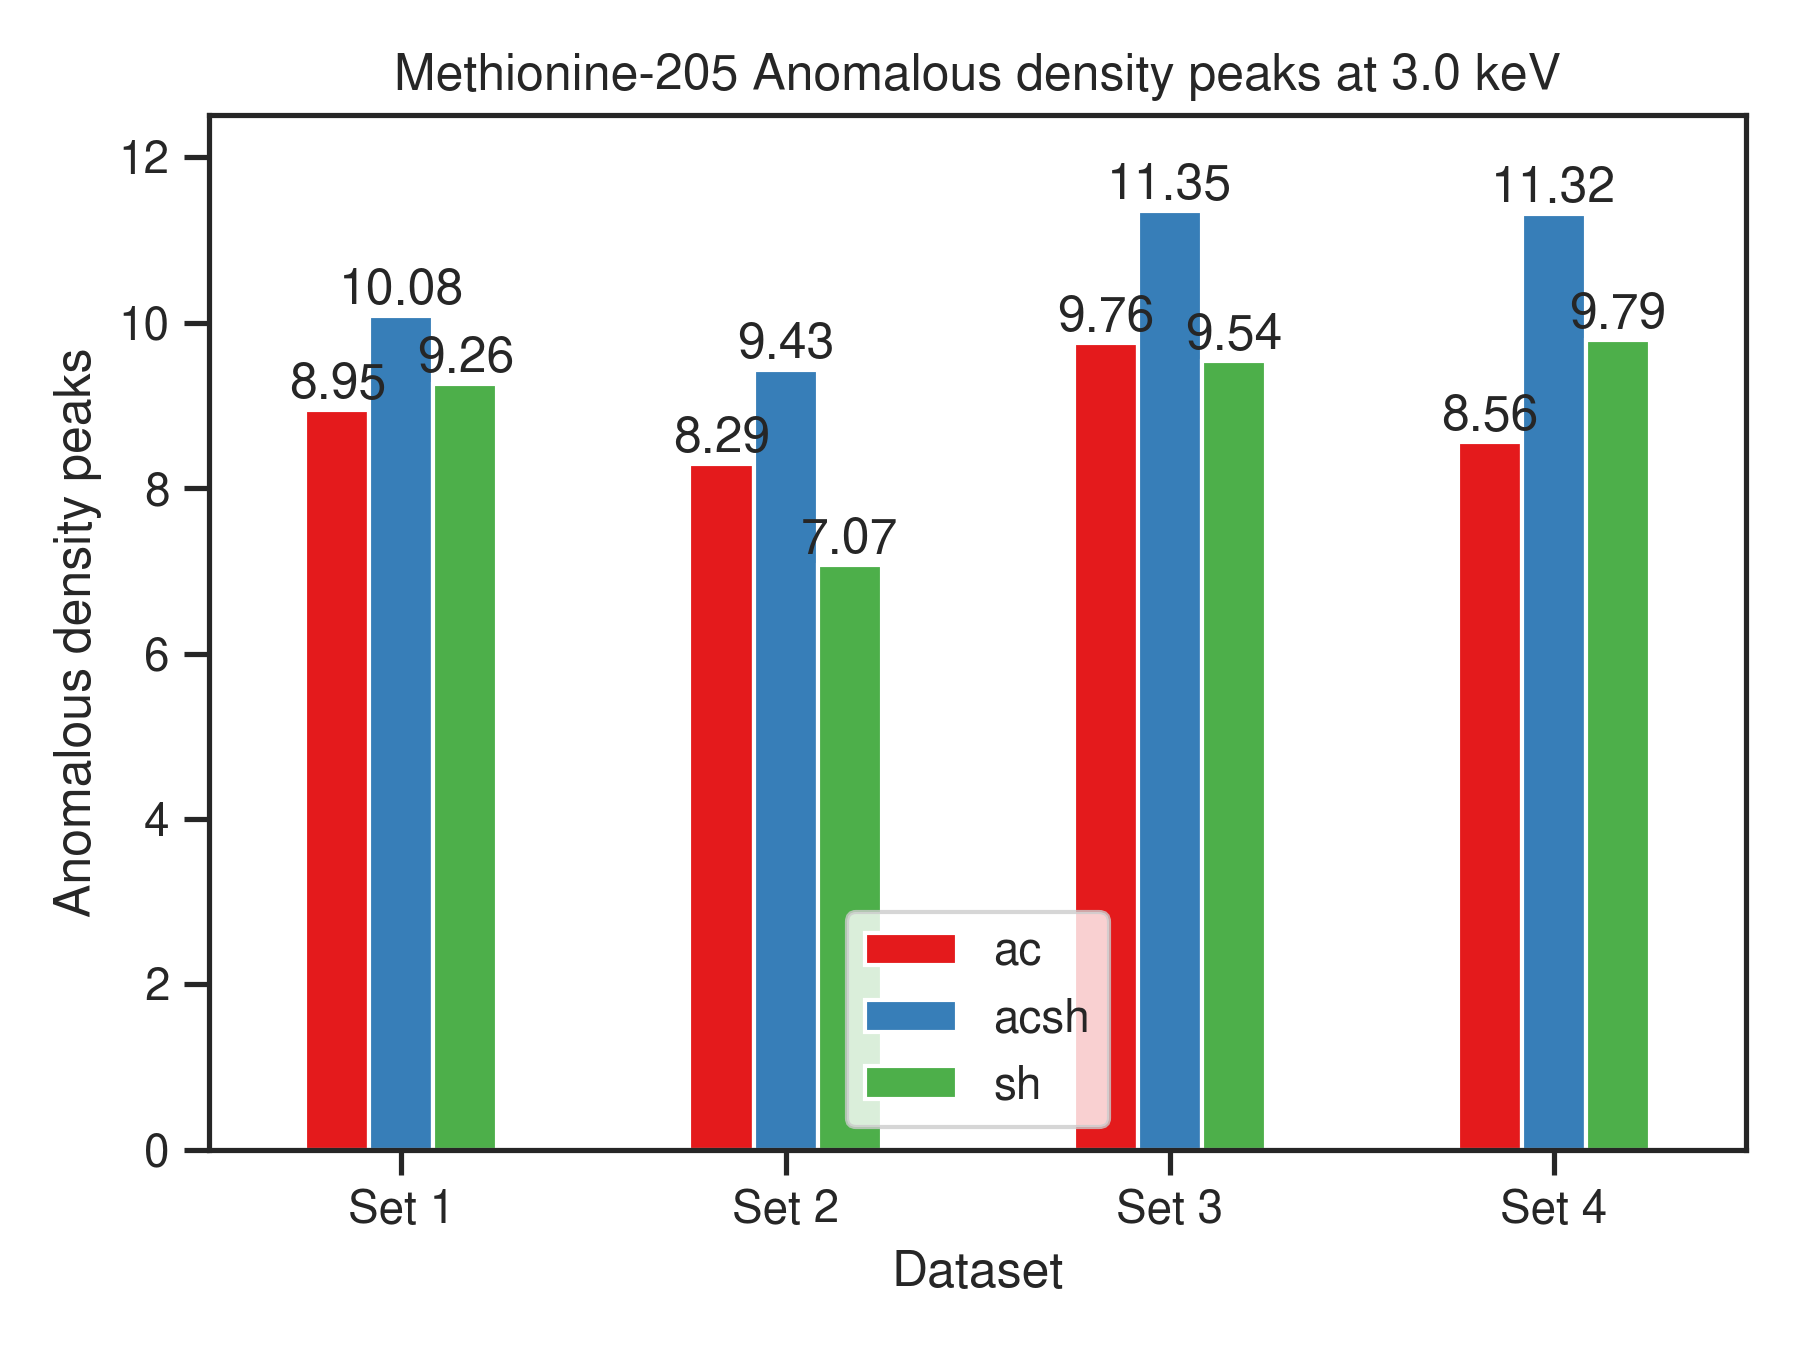
\includegraphics[width = 0.5\textwidth]{plots/exp1/tlys_9_P6122/peaks/3p0_met205_peaks.png}
    \end{tabular}
    \caption{Thermolysin 1: Anomalous density peaks of methionine groups at 3.0 \unit{keV}.}
    \label{fig:tlys9_met_peaks_3p0}
\end{figure}

\begin{figure}
    \centering
    \begin{tabular}{cc}
        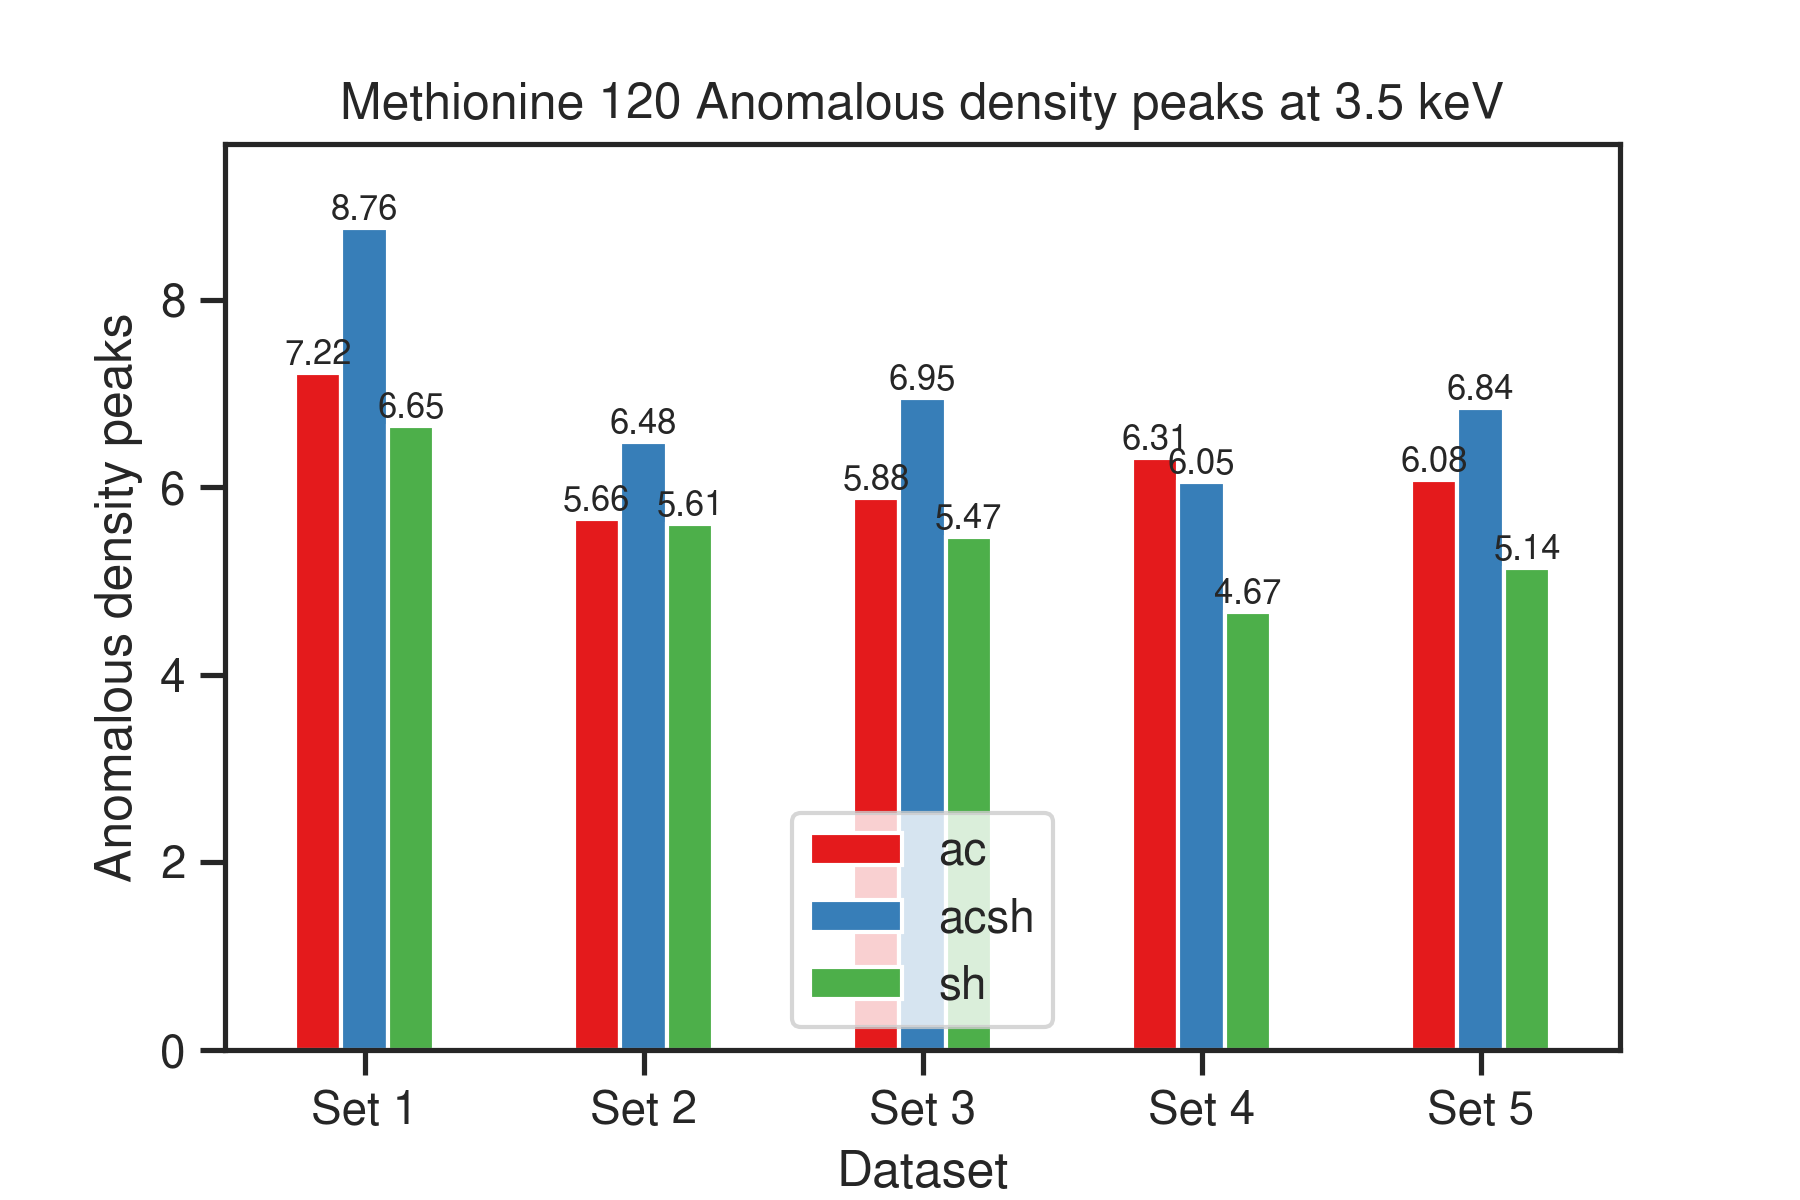
\includegraphics[width = 0.5\textwidth]{plots/exp1/tlys_9_P6122/peaks/3p5_met120_peaks.png} & 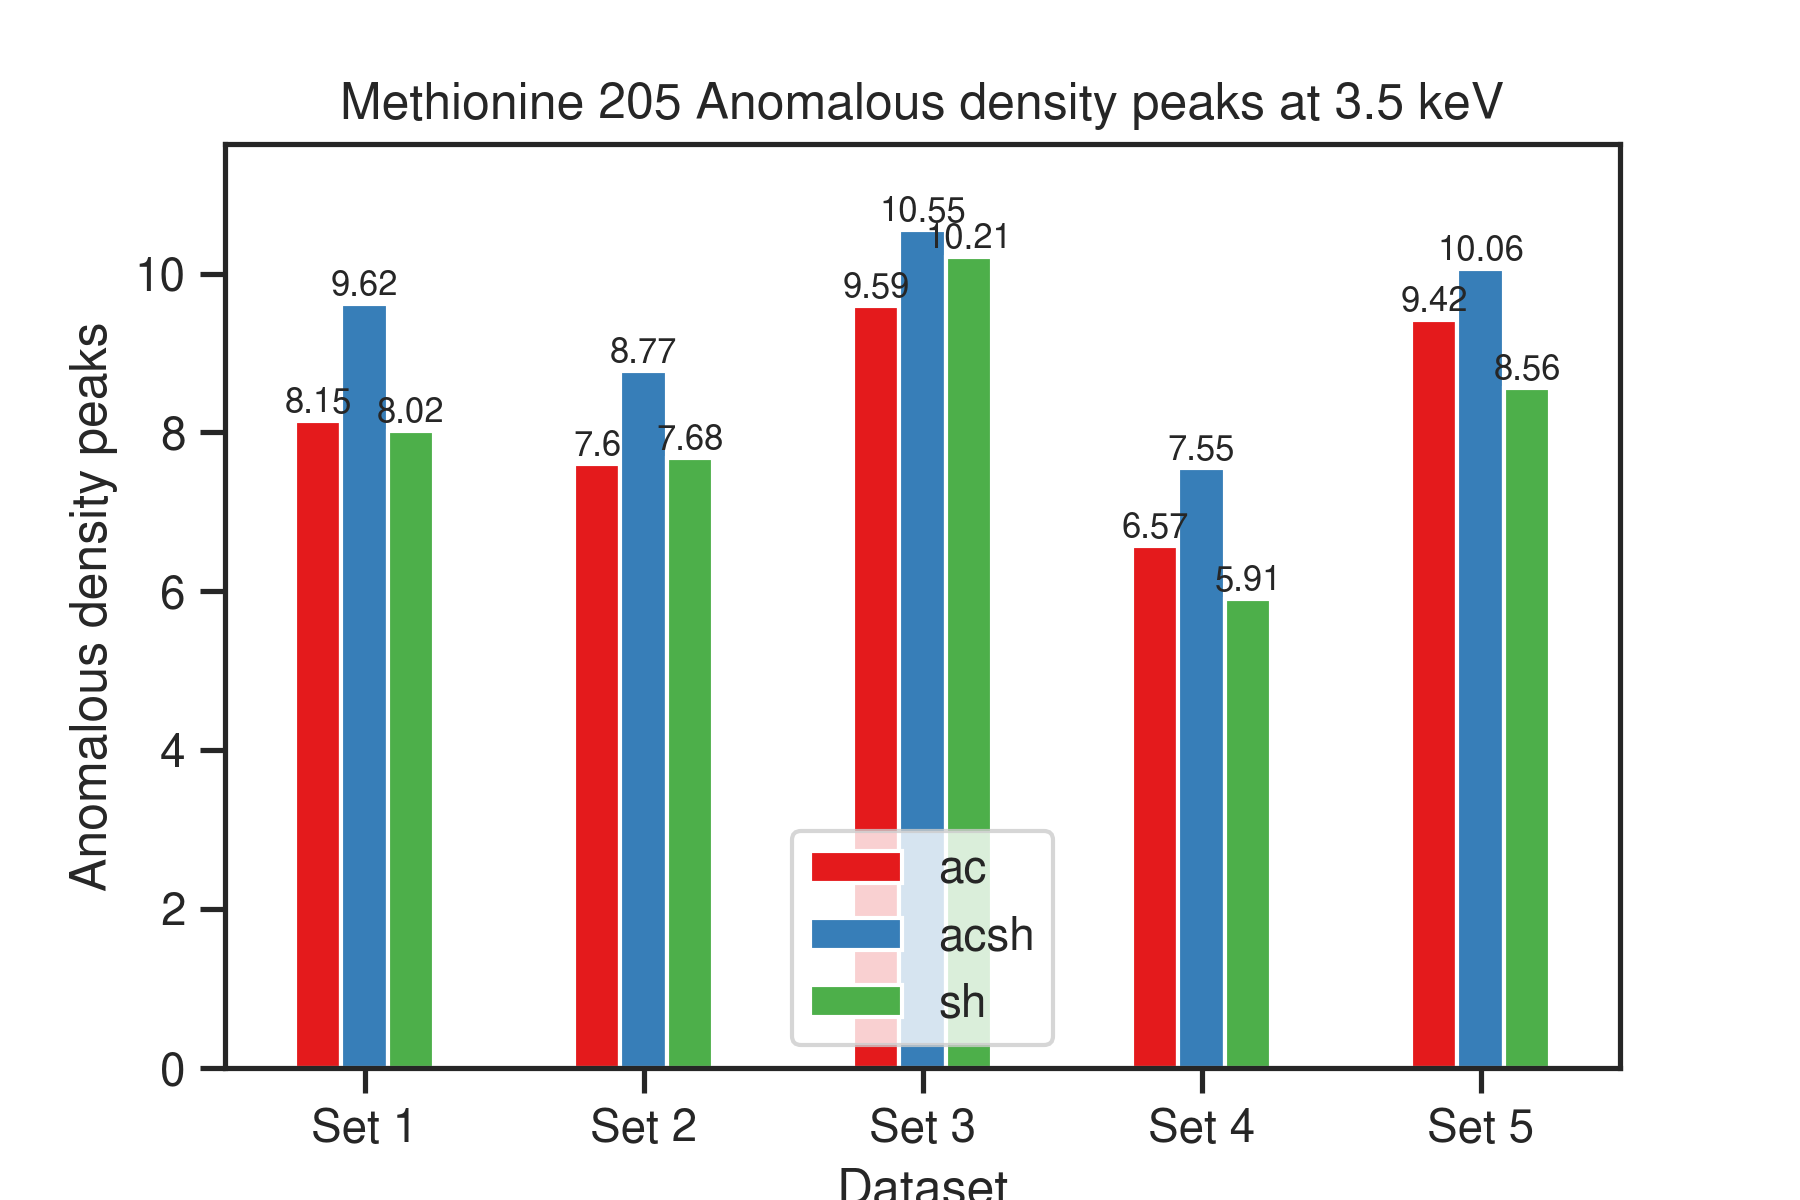
\includegraphics[width = 0.5\textwidth]{plots/exp1/tlys_9_P6122/peaks/3p5_met205_peaks.png}
    \end{tabular}
    \caption{Thermolysin 1: Anomalous density peaks of methionine groups at 3.5 \unit{keV}.}
    \label{fig:tlys9_met_peaks_3p5}
\end{figure}

\begin{figure}
    \centering
    \begin{tabular}{cc}
        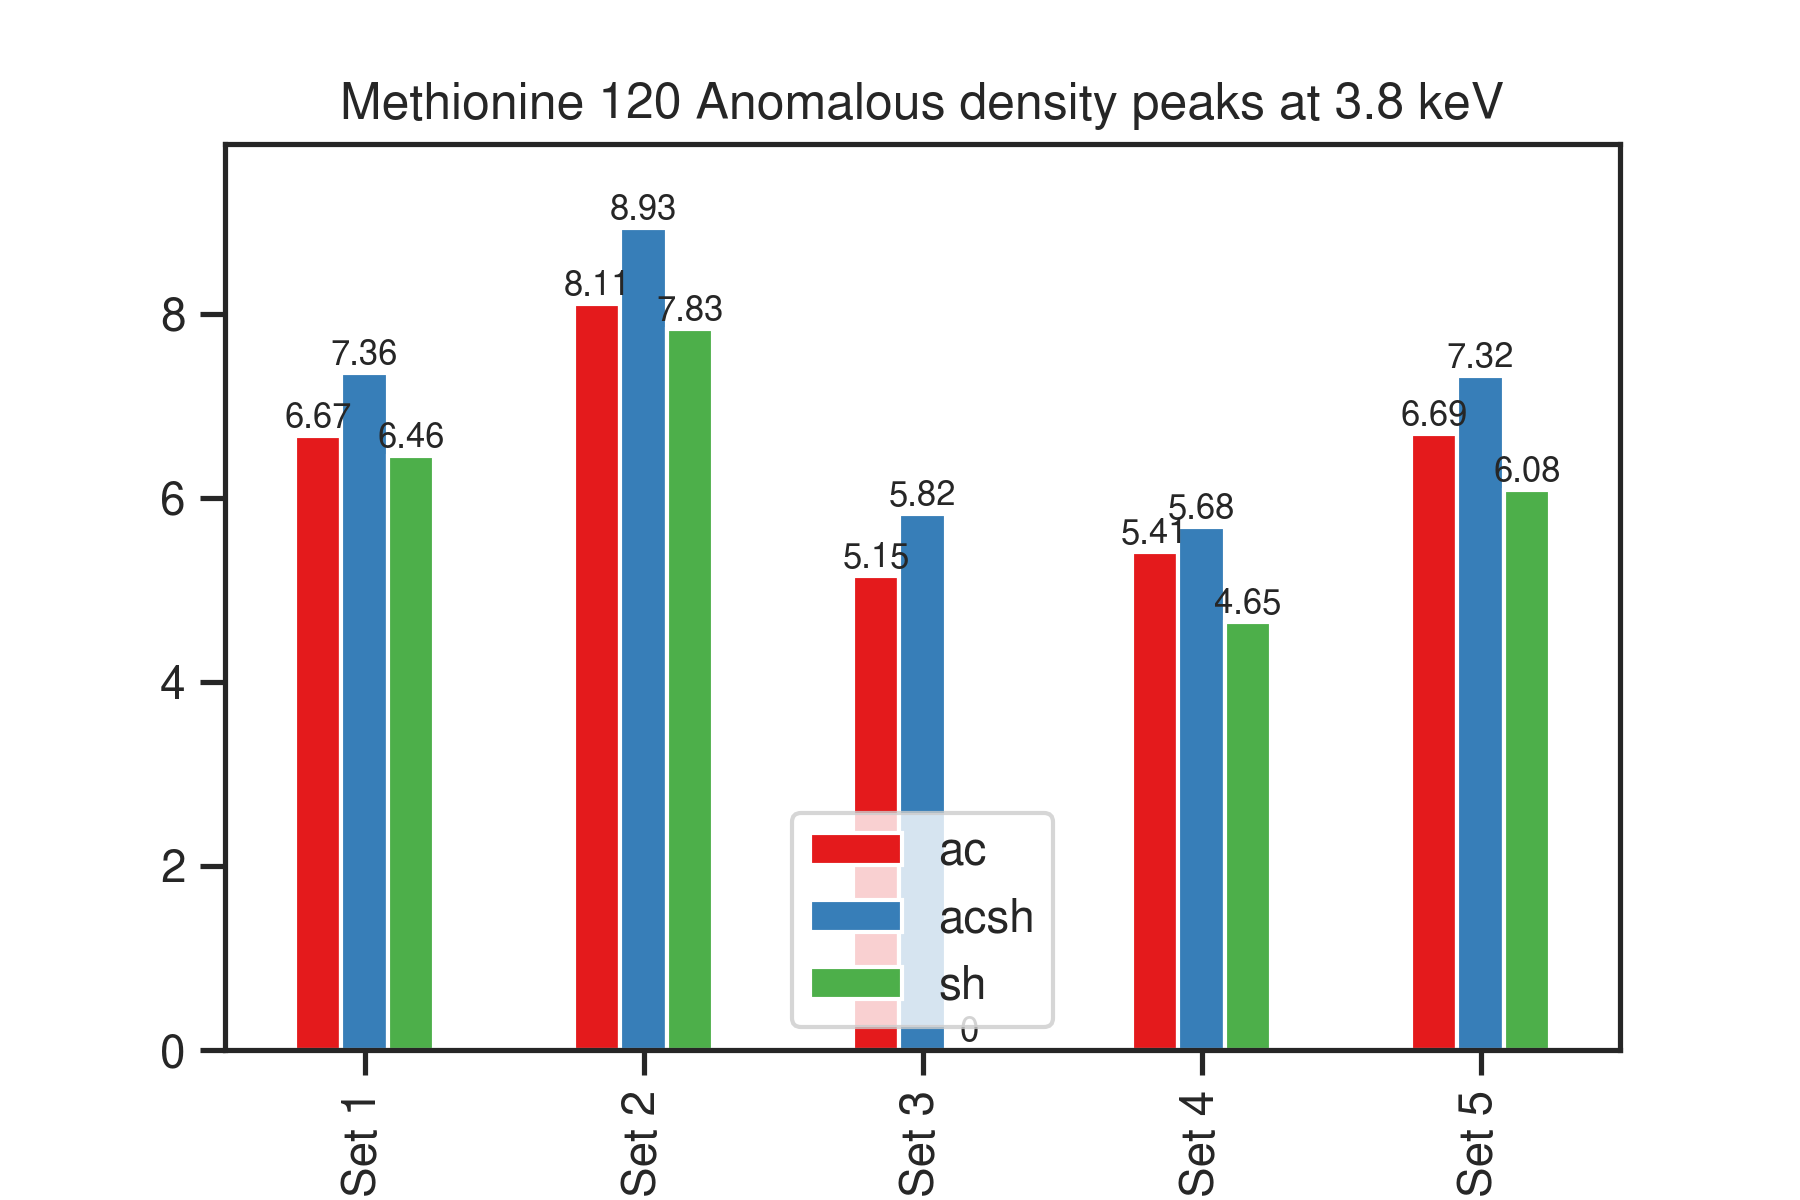
\includegraphics[width = 0.5\textwidth]{plots/exp1/tlys_9_P6122/peaks/3p8_met120_peaks.png} & 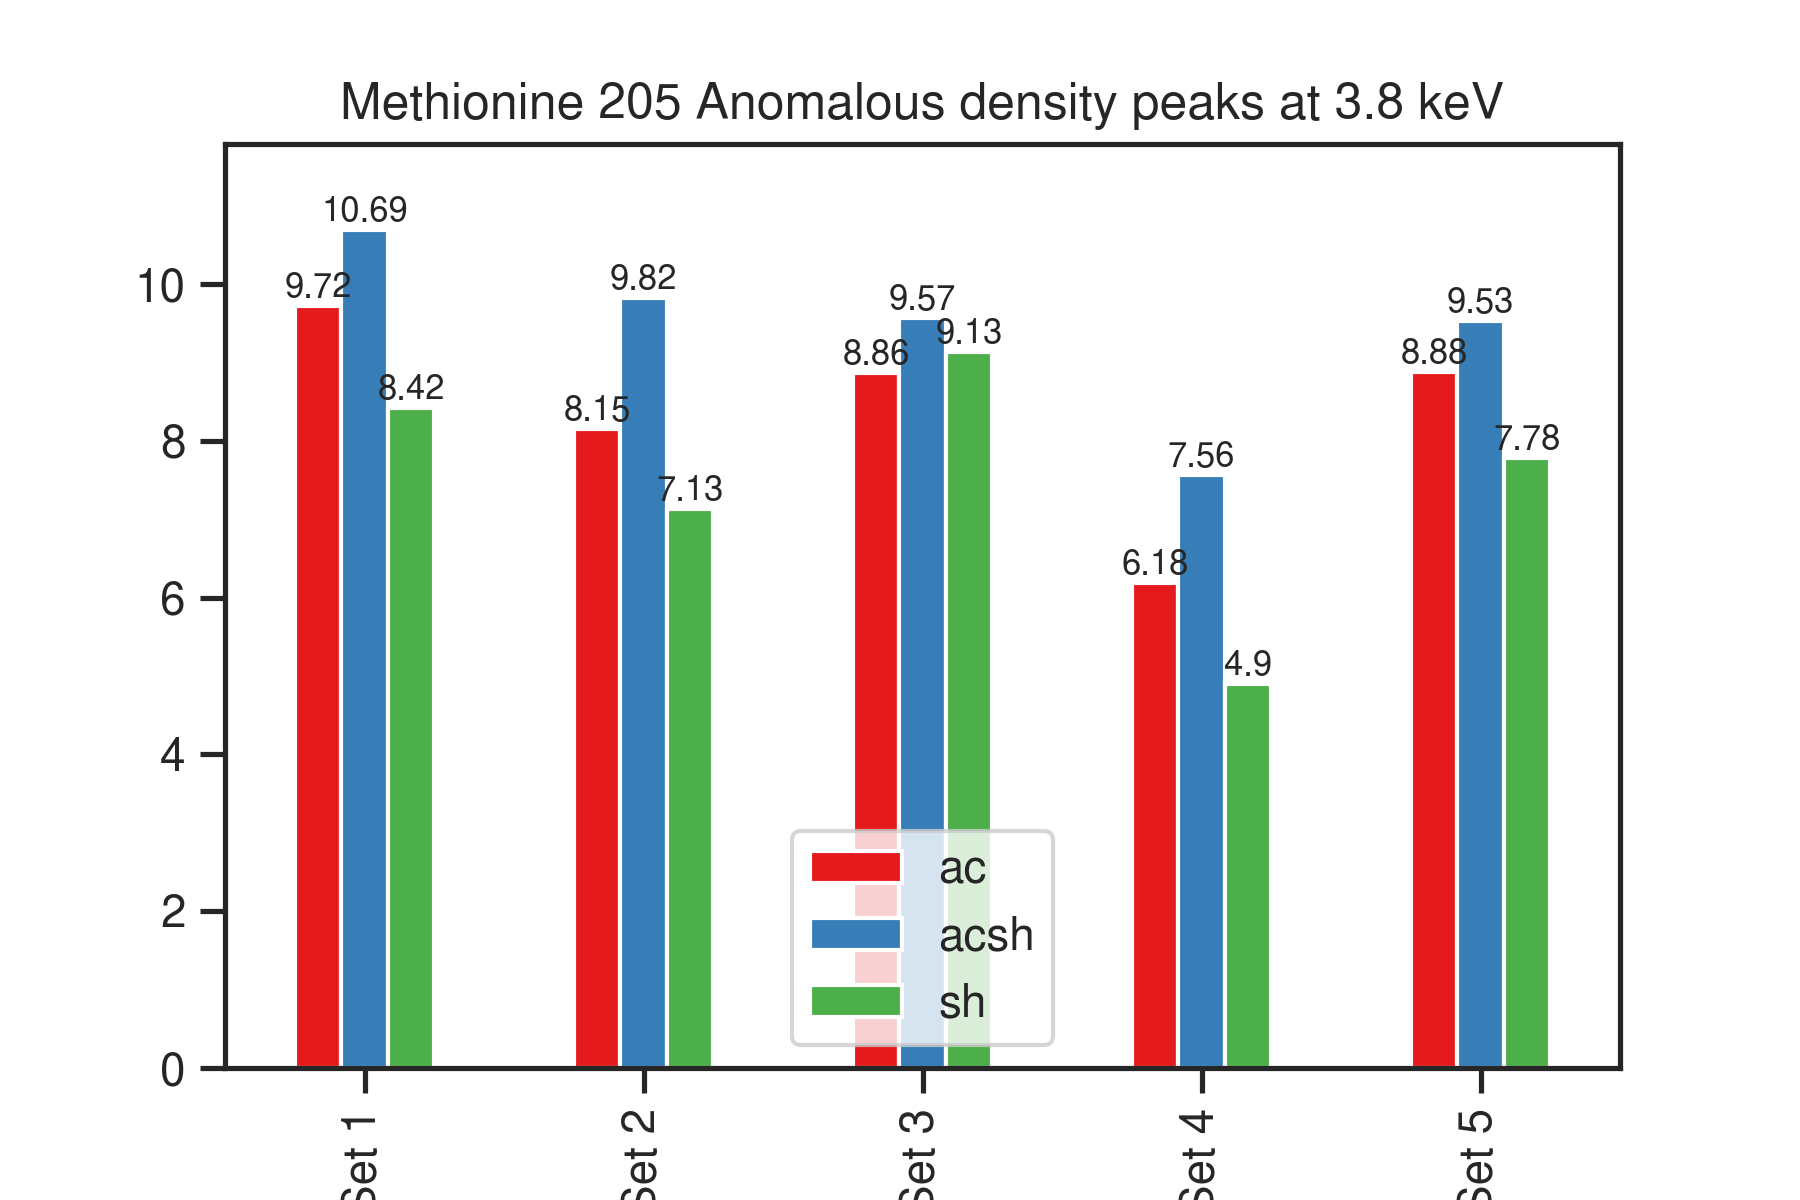
\includegraphics[width = 0.5\textwidth]{plots/exp1/tlys_9_P6122/peaks/3p8_met205_peaks.png}
    \end{tabular}
    \caption{Thermolysin 1: Anomalous density peaks of methionine groups at 3.8 \unit{keV}.}
    \label{fig:tlys9_met_peaks_3p8}
\end{figure}

\begin{figure}
    \centering
    \begin{tabular}{cc}
        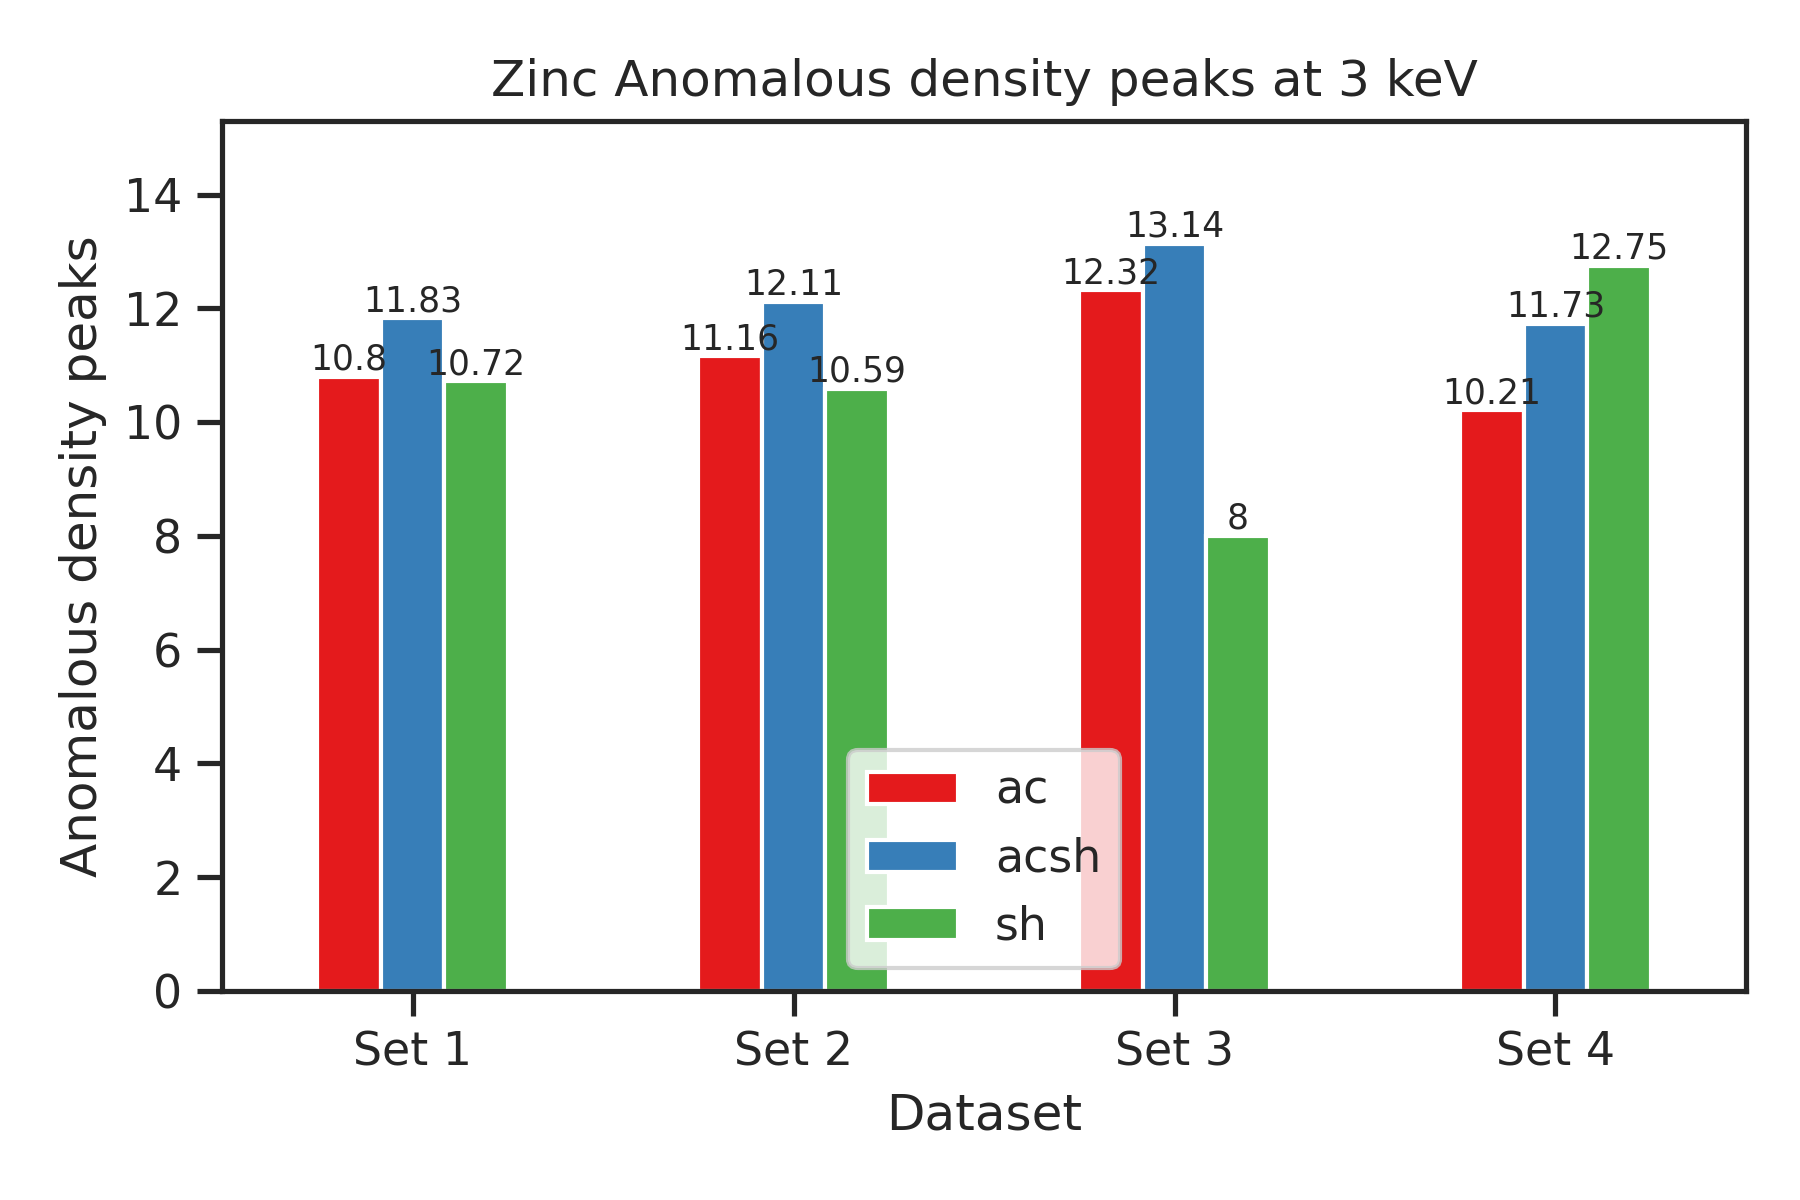
\includegraphics[width = 0.5\textwidth]{plots/exp1/tlys_2_P6122/peaks/3p0_zn_2Dbar.png} & 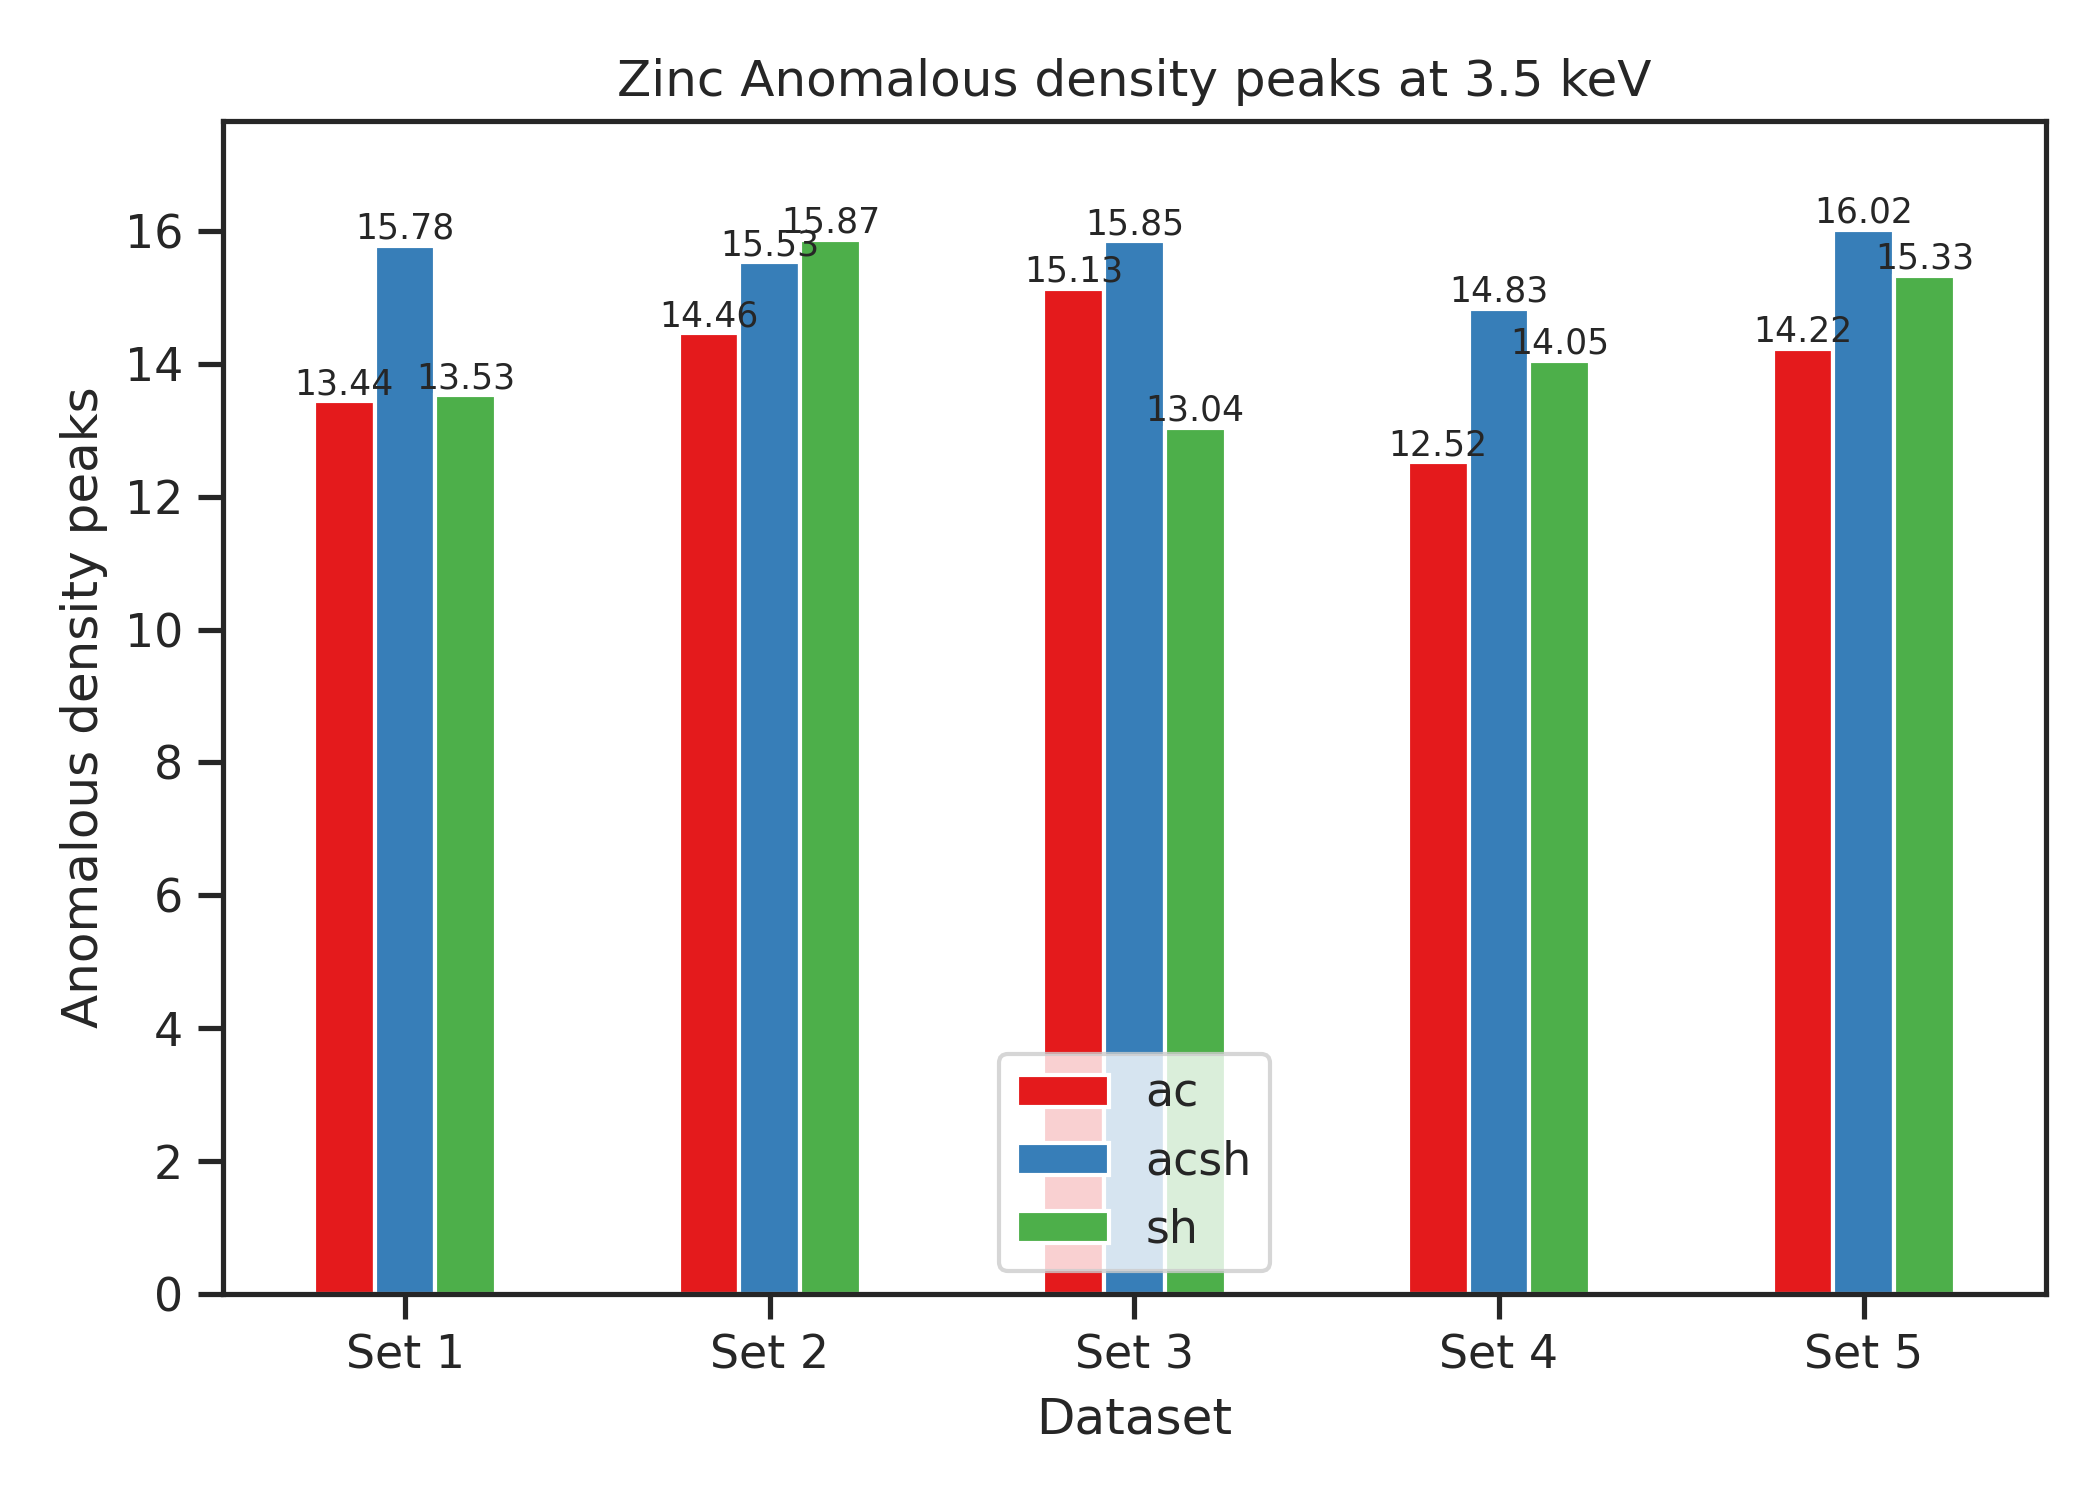
\includegraphics[width = 0.5\textwidth]{plots/exp1/tlys_2_P6122/peaks/3p5_zn_2Dbar.png}
    \end{tabular}
    \caption{Thermolysin 1: Anomalous density peaks of Zinc at 3.0 and 3.5 \unit{keV}.}
    \label{fig:tlys9_zn_peaks_3p0_3p5}
\end{figure}

\begin{figure}
    \centering
    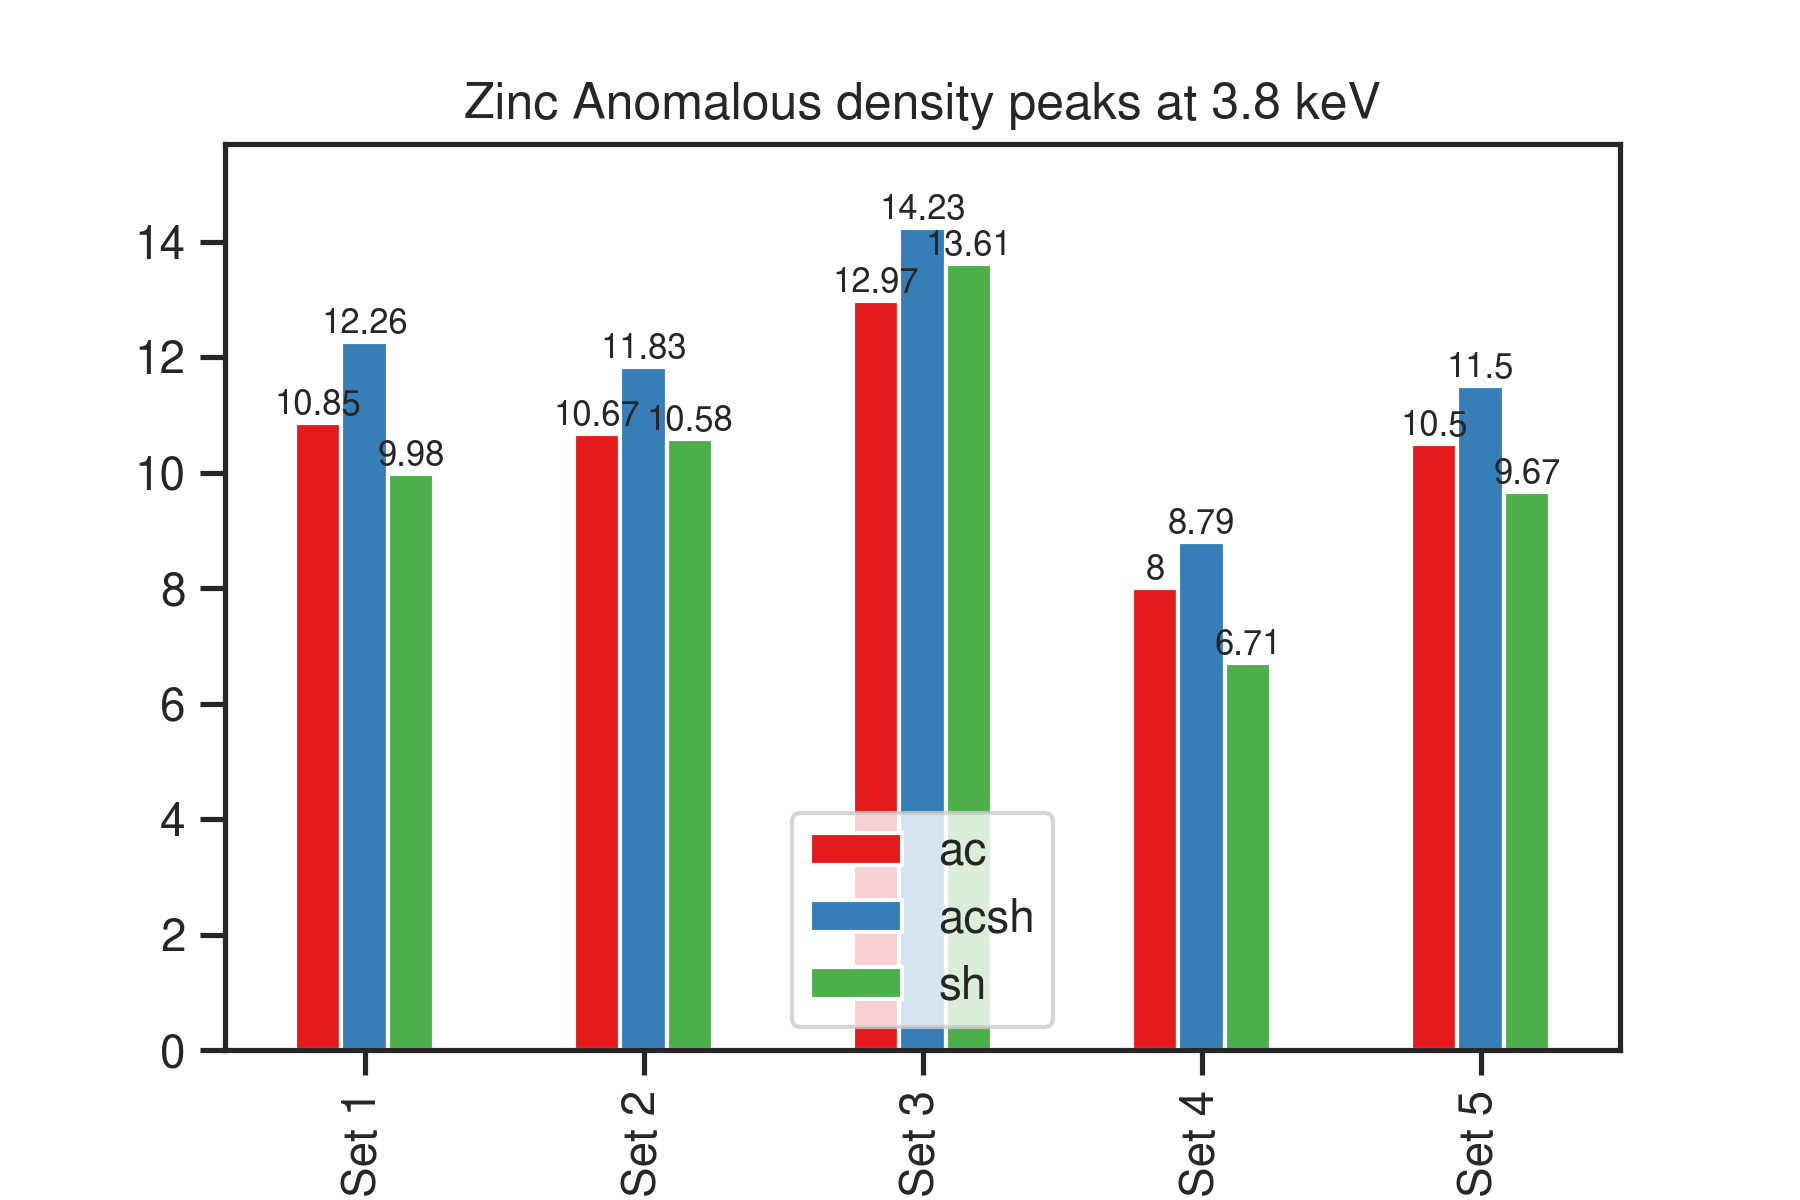
\includegraphics[width = 0.5\textwidth]{plots/exp1/tlys_9_P6122/peaks/3p8_zn405_peaks.png}
    \caption{Thermolysin 1: Anomalous density peaks of Zinc at 3.8 \unit{keV}.}
    \label{fig:tlys9_zn_peaks_3p8}
\end{figure}



% TLYS 2 ANODE PEAKS
\begin{figure}
    \centering
    \begin{tabular}{cc}
        \includegraphics[width = 0.5\textwidth]{plots/exp1/tlys_2_P6122/peaks/3p0_m120_2Dbar.png} & \includegraphics[width = 0.5\textwidth]{plots/exp1/tlys_2_P6122/peaks/3p0_m205_2Dbar.png}
    \end{tabular}
    \caption{Thermolysin 2: Anomalous density peaks of methionine groups at 3.0 \unit{keV}.}
    \label{fig:tlys2_met_peaks_3p0}
\end{figure}

\begin{figure}
    \centering
    \begin{tabular}{cc}
        \includegraphics[width = 0.5\textwidth]{plots/exp1/tlys_2_P6122/peaks/3p5_m120_2Dbar.png} & \includegraphics[width = 0.5\textwidth]{plots/exp1/tlys_2_P6122/peaks/3p5_m205_2Dbar.png}
    \end{tabular}
    \caption{Thermolysin 2: Anomalous density peaks of methionine groups at 3.5 \unit{keV}.}
    \label{fig:tlys2_met_peaks_3p5}
\end{figure}

\begin{figure}
    \centering
    \begin{tabular}{cc}
        \includegraphics[width = 0.5\textwidth]{plots/exp1/tlys_2_P6122/peaks/3p0_zn_2Dbar.png} & \includegraphics[width = 0.5\textwidth]{plots/exp1/tlys_2_P6122/peaks/3p5_zn_2Dbar.png}
    \end{tabular}
    \caption{Thermolysin 2: Anomalous density peaks of Zinc at 3.0 and 3.5 \unit{keV}.}
    \label{fig:tlys2_zn_peaks}
\end{figure}

\end{document}

